\documentclass[12pt]{report}
\usepackage{amsmath}
\usepackage{amssymb}
\usepackage{amsthm}
\usepackage{algorithm}
\usepackage{algcompatible}
\usepackage[noend]{algpseudocode}
\usepackage{fancyvrb}
\usepackage{hyperref}
\usepackage{subfigure}
\usepackage{graphicx}
\usepackage{pgfplots}
\usepackage{multirow}
\usepackage{kbordermatrix}
\usepackage{siunitx}
\usepackage[framemethod=tikz]{mdframed}

\definecolor{mycolor}{rgb}{0.122, 0.435, 0.698}

\newmdenv[innerlinewidth=0.5pt, roundcorner=4pt,linecolor=mycolor,innerleftmargin=6pt, innerrightmargin=6pt,innertopmargin=6pt,innerbottommargin=6pt]{mybox}


\pgfplotsset{
    compat=1.15,
    %every axis legend/.append style={at={(0.5,-0.13)},anchor=north,legend cell align=left},
    legend pos=north west,
    legend style={draw=none,
              text width=0.9in,           %% adjust
              %minimum height=0.5in,     %% adjust
              %anchor=center,
              %cells={anchor=west},
            },
    %axis lines=left,
}

\usepackage{tikz}
\usetikzlibrary{arrows, automata,calc}
\usetikzlibrary{er,positioning}
\tikzstyle{block} = [rectangle, draw, fill=blue!20, 
    text width=6em, text centered, rounded corners, minimum height=4em]
\tikzstyle{line} = [draw, -latex']

\newcommand\irregularcircle[2]{% radius, irregularity
  \pgfextra {\pgfmathsetmacro\len{(#1)+rand*(#2)}}
  +(0:\len pt)
  \foreach \a in {10,20,...,350}{
    \pgfextra {\pgfmathsetmacro\len{(#1)+rand*(#2)}}
    -- +(\a:\len pt)
  } -- cycle
}

\usepackage{ifthen}

\newcommand{\currentScope}{}
\newcommand{\currentSort}{}
\newcommand{\currentSortLabel}{}
\newcommand{\currentAlign}{}
\newcommand{\currentSize}{}

\newcounter{la}
\newcommand{\TSetSortLabel}[2]{
  \expandafter\repcommand\expandafter{\csname TUserSort@#1\endcsname}{#2}
}
\newcommand{\TSort}[4]{
  \renewcommand{\currentScope}{#1}
  \renewcommand{\currentSort}{#2}
  \renewcommand{\currentSize}{#3}
  \renewcommand{\currentAlign}{#4}
  \ifcsname TUserSort@\currentSort\endcsname
    \renewcommand{\currentSortLabel}{\csname TUserSort@\currentSort\endcsname}
  \else
    \renewcommand{\currentSortLabel}{\currentSort}
  \fi
  \begin{scope}[shift={\currentScope}]
  \ifthenelse{\equal{\currentAlign}{l}}{
    \filldraw[process box] (-0.5,-0.5) rectangle (0.5,\currentSize-0.5);
    \node[sort] at (-0.2,\currentSize-0.4) {\currentSortLabel};
   }{\ifthenelse{\equal{\currentAlign}{r}}{
     \filldraw[process box] (-0.5,-0.5) rectangle (0.5,\currentSize-0.5);
     \node[sort] at (0.2,\currentSize-0.4) {\currentSortLabel};
   }{
    \filldraw[process box] (-0.5,-0.5) rectangle (\currentSize-0.5,0.5);
    \ifthenelse{\equal{\currentAlign}{t}}{
      \node[sort,anchor=east] at (-0.3,0.2) {\currentSortLabel};
    }{
      \node[sort] at (-0.6,-0.2) {\currentSortLabel};
    }
   }}
  \setcounter{la}{\currentSize}
  \addtocounter{la}{-1}
  \foreach \i in {0,...,\value{la}} {
    \TProc{\i}
  }
  \end{scope}
}

\newcommand{\TTickProc}[2]{ % pos, label
  \ifthenelse{\equal{\currentAlign}{l}}{
    \draw[tick] (-0.6,#1) -- (-0.4,#1);
    \node[tick label, anchor=east] at (-0.55,#1) {#2};
   }{\ifthenelse{\equal{\currentAlign}{r}}{
    \draw[tick] (0.6,#1) -- (0.4,#1);
    \node[tick label, anchor=west] at (0.55,#1) {#2};
   }{
    \ifthenelse{\equal{\currentAlign}{t}}{
      \draw[tick] (#1,0.6) -- (#1,0.4);
      \node[tick label, anchor=south] at (#1,0.55) {#2};
    }{
      \draw[tick] (#1,-0.6) -- (#1,-0.4);
      \node[tick label, anchor=north] at (#1,-0.55) {#2};
    }
   }}
}
\newcommand{\TSetTick}[3]{
  \expandafter\repcommand\expandafter{\csname TUserTick@#1_#2\endcsname}{#3}
}

\newcommand{\myProc}[3]{
  \ifcsname TUserTick@\currentSort_#1\endcsname
    \TTickProc{#1}{\csname TUserTick@\currentSort_#1\endcsname}
  \else
    \TTickProc{#1}{#1}
  \fi
  \ifthenelse{\equal{\currentAlign}{l}\or\equal{\currentAlign}{r}}{
    \node[#2] (\currentSort_#1) at (0,#1) {#3};
  }{
    \node[#2] (\currentSort_#1) at (#1,0) {#3};
  }
}
\newcommand{\TSetProcStyle}[2]{
  \expandafter\repcommand\expandafter{\csname TUserProcStyle@#1\endcsname}{#2}
}
\newcommand{\TProc}[1]{
  \ifcsname TUserProcStyle@\currentSort_#1\endcsname
    \myProc{#1}{\csname TUserProcStyle@\currentSort_#1\endcsname}{}
  \else
    \myProc{#1}{process}{}
  \fi
}

\newcommand{\repcommand}[2]{
  \providecommand{#1}{#2}
  \renewcommand{#1}{#2}
}
\newcommand{\THit}[5]{
  \path[hit] (#1) edge[#2] (#3#4);
  \expandafter\repcommand\expandafter{\csname TBounce@#3@#5\endcsname}{#4}
}
\newcommand{\TBounce}[4]{
  (#1\csname TBounce@#1@#3\endcsname) edge[#2] (#3#4)
}

%\newcommand{\TState}[1]{
%  \foreach \proc in {#1} {
%    \node[current process] (\proc) at (\proc.center) {};
%  }
%}

\newcommand{\TState}[1]{
  \foreach \proc in {#1} {
        \node[current process] (\proc) at (\proc.center) {};
  };
}
\newcommand{\TCoopHit}[6]{
  \node[#2, apdot] at (#3) {};
  \foreach \proc in {#1} {
    \draw[#2,-] (#3) edge (\proc);
  }
  \path[hit] (#3) edge[#2] (#4#5);
  \expandafter\repcommand\expandafter{\csname TBounce@#4@#6\endcsname}{#5}
}

% ex : \TAction{c_1}{a_1.west}{a_0.north west}{}{right}
% #1 = frappeur
% #2 = cible
% #3 = bond
% #4 = style frappe
% #5 = style bond
\newcommand{\TAction}[5]{
  \THit{#1}{#4}{#2}{}{#3}
  \path[bounce, bend #5=50] \TBounce{#2}{}{#3}{};
}

% ex : \TActionPlur{f_1, c_0}{a_0.west}{a_1.south west}{}{3.5,2.5}{left}
% #1 = frappeur
% #2 = cible
% #3 = bond
% #4 = style frappe
% #5 = coordonnées point central
% #6 = direction bond
\newcommand{\TActionPlur}[6]{
  \TCoopHit{#1}{#4}{#5}{#2}{}{#3}
  \path[bounce, bend #6=50] \TBounce{#2}{}{#3}{};
}

% procedure, abstractions and dependencies
\newcommand{\abstr}[1]{#1^\wedge}%\text{\textasciicircum}}
\def\BS{\mathbf{BSeq}}
\def\aBS{\abstr{\BS}}
\def\abeta{\abstr{\beta}}
\def\aZ{\abstr{\zeta}}
\def\aY{\abstr{\xi}}

\def\beforeproc{\vartriangleleft}

\def\powerset{\wp}

\def\Sce{\mathbf{Sce}}
\def\OS{\mathbf{OSeq}}
\def\Obj{\mathbf{Obj}}
%\def\Proc{\mathbf{Proc}}
%\def\Sol{\mathbf{Sol}}
\newcommand{\Sol}{\mathbf{Sol}}
\newcommand{\NSol}{\Sol}
\newcommand{\sSol}{\mathbf{Sync}}

\usepackage{galois}
\newcommand{\theOSabstr}{toOS}
\newcommand{\OSabstr}[1]{\theOSabstr(#1)}
\newcommand{\theOSconcr}{toSce}
\newcommand{\OSconcr}[1]{\theOSconcr(#1)}

% \def\gO{\mathbb{O}}
% \def\gS{\mathbb{S}}
\def\aS{\mathcal{A}}
\def\Req{\mathrm{Req}}
%\def\Sol{\mathrm{Sol}}
\def\Cont{\mathrm{Cont}}
\def\cBS{\BS_\ctx}
\def\caBS{\aBS_\ctx}
\def\caS{\aS_\ctx}
\def\cSol{\Sol_\ctx}
\def\cReq{\Req_\ctx}
\def\cCont{\Cont_\ctx}

\def\any{\star}

% \def\gProc{\mathrm{maxPROC}}
\def\mCtx{\mathrm{maxCtx}}

%\def\procs{\f{procs}}
\def\objs{\f{objs}}
\def\sat#1{\lceil #1\rceil}

\def\gCont{\f{maxCont}}
\def\lCont{\f{minCont}}
\def\lProc{\f{minProc}}
\def\gProc{\f{maxProc}}

\def\join{\oplus}
\def\concat{\!::\!}
\def\emptyseq{\varepsilon}
\def\ltw{\preccurlyeq_{\OS}}
\def\indexes#1{\mathbb{I}^{#1}}
%\def\indexes#1{\{1..|#1|\}}
\def\supp{\f{support}}
\def\w{\omega}
\def\W{\Omega}
% \def\ctx{\varsigma}
%\def\ctx{{\textcolor{green}{s}}}
% \def\ctx{s}
% \def\Ctx{\mathbf{Ctx}}
\def\Ctx{\mathbf{Ctx}}
\def\mconcr{\gamma}
\def\concr{\mconcr_s}
\def\obj#1#2{{#1\!\Rsh^*\!\!#2}}
\def\objp#1#2#3{\obj{{#1}_{#2}}{{#1}_{#3}}}
\def\A{\mathcal{A}}
\def\cwA{\A_\ctx^\w}
\def\cwReq{\Req_\ctx^\w}
\def\cwSol{\Sol_\ctx^\w}
\def\cwCont{\Cont_\ctx^\w}
\def\gCtx{\f{maxCtx}}
\def\endCtx{\f{endCtx}}
\def\ceil{\f{end}}

%\def\lfp{\mathrm{lfp}\;}
%\def\mlfp#1{\mathrm{lfp}\{#1\}\;}
\newcommand{\lfp}[3]{\mathbf{lfp}\{#1\}\left(#2\mapsto#3\right)}
\def\maxobjs{{\f{maxobjs}}}
\def\maxprocs{{\f{maxprocs}_\ctx}}
\def\objends{{\f{ends}}}

\def\ra{\rho}
\def\rb{\rho^\wedge}
\def\rc{\widetilde{\rho}}
\def\interleave{\f{interleave}}

\def\join{\concat}

\tikzstyle{aS}=[every edge/.style={draw,->,>=stealth}]
\tikzstyle{Asol}=[draw,circle,minimum size=5pt,inner sep=0,node distance=1cm]
\tikzstyle{Aproc}=[draw,node distance=1cm]
\tikzstyle{Aobj}=[node distance=1.5cm]
\tikzstyle{Anos}=[font=\Large]
\tikzstyle{Assol}=[node distance=1.2cm]
%\tikzstyle{AprocPrio}=[Aproc,double]
\tikzstyle{AsolPrio}=[Asol,double]
\tikzstyle{AprocPrio}=[Aproc,double]
\tikzstyle{aSPrio}=[aS,double]


\newcommand{\startl}[1]{\node[Aproc] (#1) {$#1$};\node[Asol,right of=#1] (#1s) {};\path (#1) edge (#1s);}%start link
\newcommand{\link}[2]{\node[Aproc,right of=#1s] (#2) {$#2$};\node[Asol,right of=#2] (#2s) {};\path (#1s) edge (#2) (#2) edge (#2s);} %normal link
\newcommand{\specl}[3]{\node[Aproc,#1 right of=#2s] (#3) {$#3$};\node[Asol,right of=#3] (#3s) {};\path (#2s) edge (#3) (#3) edge (#3s);} %special link
\newcommand{\edl}[2]{\node[Assol,right of=#1s] (#1st){$\varnothing$};\path (#1s) edge (#1st);}%end link


%\def\procs{\mathsf{procs}}
%\def\allprocs{\mathsf{allProcs}}
%\def\allprocs{\procs}
%\def\pfp{\mathsf{pfp}}
\def\pfp{\mathsf{focals}^1}
\def\pfpprocs{\mathsf{pfpProcs}}
\def\bounceprocs{\mathsf{bounceProcs}}
\def\newprocs{\mathsf{newProcs}}

\def\aB{\mathcal{B}}
\def\sat#1{{#1}}
%\def\sat#1{\lceil #1\rceil}
\newcommand{\thisB}[2]{\sat{\aB_{#2}^{#1}}}
\newcommand{\myp}{u}
%\def\cwB{\thisB{\myp}{\ctx}}
\def\cwB{\thisB{\myp}{s}}
%\def\cwB{\sat{\aB_\ctx^\w}}
%\def\cwBz{\thisB{\myp}{\ctx_0}}
\def\cwBz{\thisB{\myp}{s_0}}
\def\mycwB#1#2{\sat{\aB_{#1}^{#2}}}
\def\Bsol{\sat{\Sol^\w_\ctx}}
\def\Breq{\sat{\Req^\w_\ctx}}
\def\Bcont{\sat{\Cont^\w_\ctx}}

\def\myB{\aB^\myp_\ctx}
\def\mysol{\overline{\Sol^\w_\ctx}}
\def\myreq{\overline{\Req^\w_\ctx}}
\def\mycont{\overline{\Cont^\w_\ctx}}

\newcommand{\csState}{\mathsf{procState}}

\newcommand{\V}{V}
\newcommand{\E}{E}
\newcommand{\cwV}{\V_s^\myp}
\newcommand{\cwE}{\E_s^\myp}
% \newcommand{\cwV}{\V_\ctx^\myp}
% \newcommand{\cwE}{\E_\ctx^\myp}
%\newcommand{\VProc}{\textcolor{red}{\V_\PHproc}}
%\newcommand{\VObj}{\textcolor{red}{\V_\Obj}}
%\newcommand{\VSol}{\V_{Sol}}
%\newcommand{\VSol}{\textcolor{red}{\V_{\Sol}}}
\newcommand{\VProc}{\V \cap \PHproc}
\newcommand{\VObj}{\V \cap \Obj}
\newcommand{\VSol}{\V \cap \Sol}
\newcommand{\cwVProc}{\cwV \cap \PHproc}
\newcommand{\cwVObj}{\cwV \cap \Obj}
\newcommand{\cwVSol}{\cwV \cap \Sol}
\newcommand{\cwVsSol}{\cwV \cap \sSol}

\def\Bv{\sat{\cwV}}
\def\Be{\sat{\cwE}}
\def\BvProc{\textcolor{red}{\sat{\cwV}^\PHproc}}
\def\BvObj{\textcolor{red}{\sat{\cwV}^\Obj}}
%\def\BvSol{\sat{\cwV}^{Sol}}
\def\BvSol{\textcolor{red}{\sat{\cwV}^{\Sol}}}

\def\cwBNodes{\Bv}
\def\cwBEdges{\Be}
\def\nsol{\f{nsol}}
\def\conn{\f{conn}}

\newcommand{\Bee}[2]{\Be^{#1}_{#2}}

%\def\mlfp#1{\f{pppf}\{#1\}}

\def\PHobjp#1#2#3{\PHobj{{#1}_{#2}}{{#1}_{#3}}}
\def\Obj{\mathbf{Obj}}
\def\powerset{\wp}
\def\gCont{\f{maxCont}}

\def\muconcr{\ell}
\def\uconcr{\muconcr_\ctx}

% Styles TikZ et couleurs personnalisées

\usepackage{tikz}

\newdimen\pgfex
\newdimen\pgfem
\usetikzlibrary{arrows,shapes,shadows,scopes}
\usetikzlibrary{positioning}
\usetikzlibrary{matrix}
\usetikzlibrary{decorations.text}
\usetikzlibrary{decorations.pathmorphing}
\usetikzlibrary{arrows,shapes}

\definecolor{lightgray}{rgb}{0.8,0.8,0.8}
\definecolor{lightgrey}{rgb}{0.8,0.8,0.8}

\definecolor{lightred}{rgb}{1,0.8,0.8}
\definecolor{lightgreen}{rgb}{0.7,1,0.7}
\definecolor{darkgreen}{rgb}{0,0.5,0}
\definecolor{darkblue}{rgb}{0,0,0.5}
\definecolor{darkyellow}{rgb}{0.5,0.5,0}
\definecolor{lightyellow}{rgb}{1,1,0.6}
\definecolor{darkcyan}{rgb}{0,0.6,0.6}
\definecolor{lightcyan}{rgb}{0.6,1,1}
\definecolor{darkorange}{rgb}{0.8,0.2,0}
\definecolor{notsodarkred}{rgb}{0.8,0,0}

\definecolor{notsodarkgreen}{rgb}{0,0.7,0}

%\definecolor{coloract}{rgb}{0,1,0}
%\definecolor{colorinh}{rgb}{1,0,0}
\colorlet{coloract}{darkgreen}
\colorlet{colorinh}{red}
\colorlet{coloractgray}{lightgreen}
\colorlet{colorinhgray}{lightred}
\colorlet{colorinf}{darkgray}
\colorlet{coloractgray}{lightgreen}
\colorlet{colorinhgray}{lightred}

\colorlet{colorgray}{lightgray}
\colorlet{colorhl}{blue}


\tikzstyle{boxed ph}=[]
\tikzstyle{sort}=[fill=lightgray, rounded corners, draw=black]
\tikzstyle{process}=[circle,draw,minimum size=15pt,fill=white,font=\footnotesize,inner sep=1pt]
%\tikzstyle{black process}=[process, draw=blue, fill=red,text=black,font=\bfseries]
\tikzstyle{gray process}=[process, draw=black, fill=lightgray]
\tikzstyle{highlighted process}=[current process, fill=gray]
\tikzstyle{process box}=[fill=none,draw=black,rounded corners]
\tikzstyle{current process}=[process, draw=black, fill=lightgray]
%\tikzstyle{current process}=[process,fill=lightcyan]
\tikzstyle{hl process}=[process,fill=blue!30]
\tikzstyle{tick label}=[font=\footnotesize]
\tikzstyle{tick}=[densely dotted] %-
\tikzstyle{hit}=[->,>=angle 45]
\tikzstyle{selfhit}=[min distance=50pt,curve to]
\tikzstyle{bounce}=[densely dotted,>=stealth',->]
\tikzstyle{ulhit}=[draw=lightgray,fill=lightgray]
\tikzstyle{pulhit}=[fill=lightgray]
\tikzstyle{bulhit}=[draw=lightgray]
\tikzstyle{hl}=[very thick,colorhl]
\tikzstyle{hlb}=[very thick]
\tikzstyle{hlhit}=[hl]
%\tikzstyle{hl2}=[hl]
%\tikzstyle{nohl}=[font=\normalfont,thin]

\tikzstyle{update}=[draw,->,dashed,shorten >=.7cm,shorten <=.7cm]

\tikzstyle{unprio}=[draw,thin]%[double]
%\tikzstyle{prio}=[draw,thick,-stealth]%[double]
\tikzstyle{prio}=[draw,-stealth,double]

\tikzstyle{hitless graph}=[every edge/.style={draw=red,-}]

\tikzstyle{aS}=[every edge/.style={draw,->,>=stealth}]
\tikzstyle{Asol}=[draw,circle,minimum size=5pt,inner sep=0,node distance=1cm]
\tikzstyle{Aproc}=[draw,node distance=1.2cm]
\tikzstyle{Aobj}=[node distance=1.5cm]
\tikzstyle{Anos}=[font=\Large]

\tikzstyle{AsolPrio}=[Asol,double]
\tikzstyle{AprocPrio}=[Aproc,double]
\tikzstyle{aSPrio}=[aS,double]

\colorlet{colorhlwarn}{notsodarkred}
\colorlet{colorhlwarnbg}{lightred}
\tikzstyle{Ahl}=[very thick,fill=colorhlwarnbg,draw=colorhlwarn,text=colorhlwarn]
\tikzstyle{Ahledge}=[very thick,double=colorhlwarnbg,draw=colorhlwarn,color=colorhlwarn]





%\definecolor{darkred}{rgb}{0.5,0,0}



\tikzstyle{grn}=[every node/.style={circle,draw=black,outer sep=2pt,minimum
                size=15pt,text=black}, node distance=1.5cm, ->]
\tikzstyle{inh}=[>=|,-|,draw=colorinh,thick, text=black,label]
\tikzstyle{act}=[->,>=triangle 60,draw=coloract,thick,color=coloract]
\tikzstyle{inhgray}=[>=|,-|,draw=colorinhgray,thick, text=black,label]
\tikzstyle{actgray}=[->,>=triangle 60,draw=coloractgray,thick,color=coloractgray]
\tikzstyle{inf}=[->,draw=colorinf,thick,color=colorinf]
%\tikzstyle{elabel}=[fill=none, above=-1pt, sloped,text=black, minimum size=10pt, outer sep=0, font=\scriptsize,draw=none]
\tikzstyle{elabel}=[fill=none,text=black, above=-2pt,%sloped,
minimum size=10pt, outer sep=0, font=\scriptsize, draw=none]
%\tikzstyle{elabel}=[]


\tikzstyle{plot}=[every path/.style={-}]
\tikzstyle{axe}=[black,->,>=stealth']
\tikzstyle{ticks}=[font=\scriptsize,every node/.style={black}]
\tikzstyle{mean}=[thick]
\tikzstyle{interval}=[line width=5pt,red,draw opacity=0.7]
%\definecolor{lightred}{rgb}{1,0.3,0.3}

%\tikzstyle{hl}=[yellow]
%\tikzstyle{hl2}=[orange]

%\tikzstyle{every matrix}=[ampersand replacement=\&]
%\tikzstyle{shorthandoff}=[]
%\tikzstyle{shorthandon}=[]
\tikzstyle{objective}=[process,very thick,fill=yellow!50]

\tikzstyle{coopupdate}=[-stealth,decorate,decoration={zigzag,amplitude=1.5pt,post=lineto,post length=.3cm,pre=lineto,pre length=.3cm}]

\tikzstyle{labelprio}=[circle, fill=blue!30, inner sep=0pt, minimum size=13pt]
\tikzstyle{labelprio1}=[labelprio]
\tikzstyle{labelprio2}=[labelprio, fill=red!60]
\tikzstyle{labelprio3}=[labelprio, fill=orange!50]
\tikzstyle{labelprio4}=[labelprio, fill=brown!50]

\tikzstyle{labelstocha}=[rectangle, rounded corners=4pt]

\tikzstyle{andot}=[circle, fill=black, inner sep=1.2pt, draw=transparent]
\tikzstyle{anligne}=[thick]

\tikzstyle{apdot}=[andot] %[circle, fill=black, draw=black, inner sep=1]
\tikzstyle{apdotsimple}=[] %[circle, fill=black, draw=black, inner sep=1]

% Figure de résumé des liens entre les formalismes
\tikzstyle{equiv-externe}=[thick, rounded corners, draw=gray, fill=gray!10, align=center,
  inner sep=8]

% label pour les délais des actions 
 \tikzstyle{labeldelai1}=[circle, fill=red!60, inner sep=0pt, minimum size=8pt]
  \tikzstyle{labeldelai2}=[circle, fill=blue!30, inner sep=0pt, minimum size=8pt]
  \tikzstyle{labeldelai3}=[circle, fill=brown!50, inner sep=0pt, minimum size=8pt]
  \tikzstyle{labeldelai4}=[circle, fill=green!50, inner sep=0pt, minimum size=8pt]
  
% Automata Networks:
\tikzstyle{local transitions}=[->,>=latex',thick,bend left=30,
               every node/.style={fill=white,inner sep=1pt,outer sep=1pt}]
\tikzstyle{reach}=[fill=lightgray,ellipse]

\tikzstyle{local transitions 2}=[->,>=latex',thick,bend left=100,
               every node/.style={fill=white,inner sep=1pt,outer sep=4pt}]

\tikzstyle{local transitions 3}=[->,>=latex',thick,bend right=100,
               every node/.style={ right, fill=white,inner sep=1pt,outer sep=4pt}]
               
% Graphe d'états
% noeuds
\tikzstyle{vide}= [rectangle, minimum width=2em,minimum height=1.5em,]
\tikzstyle{stable}= [rectangle,fill=lightred]
\tikzstyle{current}= [rectangle,fill=lightcyan]
\tikzstyle{initial}= [rectangle,fill=green!20]

% % STG transitions
\tikzstyle{etiquette}=[midway,fill=blue!20,circle,scale=0.7pt]
\tikzstyle{etiquette2}=[midway,fill=green!20,circle,scale=0.7pt]
%
\tikzstyle{currentTrans}=[->,very thick,blue]
\tikzstyle{seperatedTransPart1}=[draw, thick, blue]
\tikzstyle{seperatedTransPart2}=[->, thick, blue]


\tikzstyle{mytext}=[thick, text width=4.5em,inner sep=1pt]
\tikzstyle{line} =[draw, thick, -latex',shorten >=2pt]
\tikzstyle{block} =[rectangle,text width=6em,draw,minimum height=4em, outer sep=0pt]

\tikzstyle{adn}=[every node/.style={circle,draw=black,outer sep=2pt,minimum
                size=15pt,text=black}, node distance=1.5cm, ->]
                
% Définition des nouvelles options xmin, xmax, ymin, ymax
% Valeurs par défaut : -3, 3, -3, 3
\tikzset{
    xmin/.store in=\xmin, xmin/.default=-3, xmin=-3,
    xmax/.store in=\xmax, xmax/.default=3, xmax=3,
    ymin/.store in=\ymin, ymin/.default=-3, ymin=-3,
    ymax/.store in=\ymax, ymax/.default=3, ymax=3,
}
% Commande qui trace la grille entre (xmin,ymin) et (xmax,ymax)
\newcommand {\grille}
    {\draw[help lines] (\xmin,\ymin) grid (\xmax,\ymax);}
% Commande \axes
\newcommand {\axes} {
    \draw[->] (\xmin,0) -- (\xmax+0.5,0);
    \draw[->] (0,\ymin) -- (0,\ymax+0.5);
}
% Commande qui limite l’affichage à (xmin,ymin) et (xmax,ymax)
\newcommand {\fenetre}
    {\clip (\xmin,\ymin) rectangle (\xmax,\ymax);}
   
 \newcommand{\nombresCopiesParNote}
   {(0,0)(1,0)(2,2)(3,0)(4,6)(5,4)(6,7)(7,4)(8,3)(9,0)(10,1)}  
% Expression level of a
 \newcommand{\expressionDiscreteA}
   {(0,0)(1,0)(2,0)(3,0)(4,0)(4,1)(5,1)(5,0)(6,0)(7,0)(8,0)(9,0)(9,1)(10,1)(11,1)(12,1)(13,1)(13,0)(14,0)(15,0)(16,0)(17,0)(17,1)(18,1)}      
   
% Expression level of b
 \newcommand{\expressionDiscreteB}
   {(0,1)(12,1)(12,0)(18,0)} 
   
% Expression level of z
 \newcommand{\expressionDiscreteZ}
   {(0,0)(3,0)(3,1)(14,1)(14,0)(18,0)}
\makeatletter
\def\input@path{{figures/}}
\makeatother
\newcommand{\acm}[3]{\{#1\}\rightarrow#3}
\newcommand{\ac}[3]{$\{#1\}\rightarrow#3$}
\newcommand{\omesi}{^\omega_\alpha}
\newcommand{\vv}{\mathrm{v}^{val}}

\newtheorem{definition}{Definition}[chapter]
\newtheorem{theorem}{Theorem}[chapter]
\newtheorem{example}{Example}[chapter]
\newtheorem{proposition}{Proposition}[chapter]
\newtheorem{remark}{Remark}[chapter]
%\newtheorem{proof}{Proof}[chapter]

\title{Doctoral Thesis}
\date{December 2018}
\author{Xinwei Chai}
\begin{document}
\maketitle
\tableofcontents
\listoffigures
\listoftables
\begin{abstract}
    In this thesis, we investigate several modeling frameworks and study several model checking techniques.
    
\end{abstract}

\chapter*{List of symbols}
\begin{tabular}{l|l}
    $a_i$  & automaton $a$ is taking value $i$ \\
    $x::y$ &  $x$ happens just before $y$\\
    $a.next$&the successor of $a$\\
    $a.pred$ & the predecessor of $a$\\
    $A\to b_j$ & condition $A$ allows variable $b$ to reach its level $j$\\
    $\mathbb{N}$ & the set of all natural numbers
\end{tabular}

%\begin{itemize}
%    \item $a_i$ means automaton $a$ is taking value $i$
%    \item $x::y$ is sequential connector of entities $x$ and $y$, where $x$ happens just before $y$
%    \item $a.next$ is the successor of $a$; $a.pred$ is the predecessor of $a$
%\end{itemize}






\chapter{Introduction}\label{chap:intro}
\begin{mybox}
Problematics, what is our work, why this work

analysis and learning, challenges, contributions
\end{mybox}

\section{Context and Motivations}
In the studies of concurrent systems, modeling is an inevitable topic.
The modeling frameworks discussed in this thesis are all designed for biological use but they can be potentially useful in other domains, \textit{e.g.} robotics, human engineering.

Models help one to access, analyze and control the real system. 
It is a tool to help people to understand the interaction of the components in real systems and the integral behavior of the systems.

A good model is a model which

\begin{itemize}
    \item is consistent with the corresponding real system
    
    The model reproduces certain important behaviors.
    In the ideal situation, the model bisimulates the real system.
    \item is observable
    
    To allow one to verify the behaviors, the state (historical, current and future) and the mechanics of the model has to be observable.
    
    \item allows one to access the I/O of the model
    
    With full control of the I/O, we can carry some unfeasible tests in real system.
    %\item allows one to access the state (historical, current and future) of the model
    \item has related analyzers of various properties
    
    Some properties are not verifiable via finite enumeration.
    \item can be translated from/to other models 
\end{itemize}

Normally, the above metrics are self-constrained:
The finer the model is, the bigger the computational complexity is (simulation, verification, \textit{etc.}).
In this thesis, we will focus on modelings, their related analyzers of system properties and model revision based on these properties.

\subsection{Models in Computational Biology}
Bioinformaticians are interested in highly abstracted models because they need abstract representation and/or flexibility to make model compatible with unknown biological knowledge.

Tractability with big data is also important.
``Big'' can refer to two meanings: one is that biological systems can be huge, with enormous components and interactions in between; another is that the number and the size of data sets can be huge.

To model the real system, we need components to represent genes, RNA messengers, proteins, metabolites, \textit{etc}.
At this stage, we can carry out a first-step abstraction.
The synthesis of proteins is under the instruction of RNA messengers which are synthesized according to genes.
This linear process allows us to compress three entities into one.
Their inner behaviors (\textit{e.g.} protein phosphorylation, activation/inhibition of genes) are characterized by the values of the associated entities.

These values can be continuous or discrete which differentiate the modeling frameworks.

Continue values correspond directly to the measurement and can be used in the models based on the family of Ordinary Differential Equation (ODE), e.g. Stochastic Differential Equation (SDE), Delay Differential Equation (DDE).

Discrete values come from an approximation from sigmoid function to step functions. 
Sigmoid function is a monotonic function and its change rate is high around a certain point (Proof in Appendix \ref{sec:proof}).
Many biological behaviors are similar with sigmoid functions: certain entity starts to influence the system if its value goes beyond a certain threshold.
If the value is far from the threshold, it is either insufficient (low level) or saturated (high level) \cite{kauffman1969,von2000segment}.
This fact inspires scientists to study discrete models.
One can encode low level as 0 and high level as 1 or even add additional levels to represent more behaviors.

In the term of concurrency, synchronous models make components to evolve at the same time while asynchronous ones allow at most one component to evolve at one time.
Due to the fuzziness of biological system, asynchronous models are compatible with more configurations of system parameters \cite{bernot2009}.

However, the compatibility of asynchronous models is also a shortcoming as they explore more state space at each system transition compared with synchronous ones.
The exploration of state space leads to so-called state space explosion problem.
To deal with such problem, Paulev\'e \textit{et al.} proposed Process Hitting framework and its related static model checker \cite{pauleve2012} and Folschette \textit{et al.} proposed Asynchronous Automata Network enriching model semantics \cite{folschette2015}.

In this thesis, we mainly study \textbf{asynchronous discrete models} based on the models above. \textbf{what is the problem of the thesis}

Apart from modelings, another important topic is model inference (or model learning). \textbf{(why this)}
It turns the data coming from biological experiment into model parameters, given modeling framework.
In this thesis, we focus on the LFIT-based method (Learning From Interpretation Transition) proposed by Robeiro \textit{et al.} \cite{ribeiro2015learning,ribeiro2018learning,ribeiro2017inductive} as it is used in our model revisers.

\section{Problematic}


\section{Contributions}\label{sec:contribution}
The main contributions of the thesis are the followings:
\begin{itemize}
    \item Development of efficient and precise reachability analyzers based on static analysis
    %\item Design of model learners using time-series data
    \item Design of model revisers using \textit{a priori} knowledge to revise existing models
\end{itemize}

This thesis aims at solving the problems in the last sections by refining existing modeling frameworks and learning approaches:

\textbf{Reachability analyzers}

To solve both the state space explosion problem and the unsatisfying precision of pure static analysis, we developed two approaches based on static analysis with different weights on \textit{efficiency} and \textit{precision}.

\textbf{Model Revisers}

As far as we know, model revision based on reachability properties has never been considered in the literature.
According to the problems of model inference above, we designed two algorithms:
\begin{itemize}
    \item algorithm based on learning from \textbf{continuous} time-series data
    
    This algorithms uses correlation coefficients to infer the correlations between the change rate of each variable and other variables in order to suggest hypothetical regulations of the system.
    With the hypothetical regulations and \textit{a priori} biological knowledge, we can revise incomplete models by adding transitions consistent with the real system.
    \item algorithm based on learning from \textbf{discretized} time-series data
    
    The learning approach we applied is the one using Inductive Logic Programming \cite{ribeiro2018learning}.
    This approach has more strict rule constraints, the model is either consistent with the original time-series data or not.
    We try to revise the model in order to make it consistent with \textit{a priori} biological knowledge and the rule constraints at the same time.
\end{itemize}


\section{Organization of the Manuscript}
Chapter \ref{chap:stateOfTheArt} introduces the state of the art on several modeling frameworks, model checkers and different dynamics of modelings.
We are especially interested in Asynchronous Automata Network, reachability analysis and the learning from state transitions.

Chapter \ref{chap:refinement} presents our modeling framework adapted from Automata Network and its relating reachability analyzers based on static analysis.
We will focus on the inconclusive cases of pure static analysis and analyze the key components preventing from a direct solution.
We then apply some different heuristics on the the key components to solve them dynamically in order to reach a conclusive result on the reachability problem.

Chapter \ref{chap:modelInference} presents the methodology of model revision in this thesis and our model revisers mentioned above.
These model revisers perform a model selection. 
They choose a model from the candidates satisfying all the provided constraints.
However the number of candidate models can be exponential, our model revisers can shrink the search space drastically to obtain a result.

Chapter \ref{chap:test} shows some comparative and exploratory tests and their results on the approaches presented in Chapter \ref{chap:refinement} and Chapter \ref{chap:modelInference}.

Chapter \ref{chap:conclusion} concludes the whole thesis.

\chapter{State of the Art}\label{chap:stateOfTheArt}

\section{Modeling Frameworks}
Original biological problems are usually difficult to study directly due to the uncertainty and the big scale of biological systems. 
Modeling is a process of abstracting the real system into a more concise and more easily automatized system.
To solve a certain problem, an appropriate modeling framework is crucial because different models have different bias from reality and have also different advantages in computation, e.g. fix point, reachability etc.
Here I introduce several most frequent modeling frameworks and compare their advantages and disadvantages.

\subsection{Regulatory Network}\label{sec:regNetwork}
Regulatory Network (RN) has characteristics of a static network, representing the interactions between components.
It is applied in static analysis, gene expression \cite{shinozaki2003regulatory}, \textit{etc}.

\begin{definition}[Regulatory network]\label{def:RN}
A regulatory network is a labeled digraph $G=(V,E)$ where 
\begin{itemize}
    \item each vertex $v$ of $V$, called variable, is provided with a boundary $b_v\in \mathbb{N}$ less or equal to the out-degree of v in G.
    \item each arc $u\in v$ of $E$ is labelled with a couple ($t_{uv}$, $\alpha_{uv}$) where $t_{uv}$ is an integer between 1 and $b_v$, called qualitative threshold and where $\alpha_{uv}\in \{+,-\}$ is the sign of the regulation.
\end{itemize}
\end{definition}

\subsection{Boolean Network}
Boolean Network (BN) is a traditional framework studied for decades \cite{kauffman1969}.
A BN $G(V,F)$ consists of a set of nodes $V=\{v_1,\cdots,v_n\}$ and a set of Boolean functions $F=(f_1,\cdots,f_n)$ where $f_i(v_1,\cdots,v_n)$ decides the value of node $v_i$ of the next time point.
In some applications, the nodes are classified into incoming nodes, outgoing nodes and inner nodes to represent an input-output system \cite{akutsu2007control}.
\begin{figure}
    \centering
    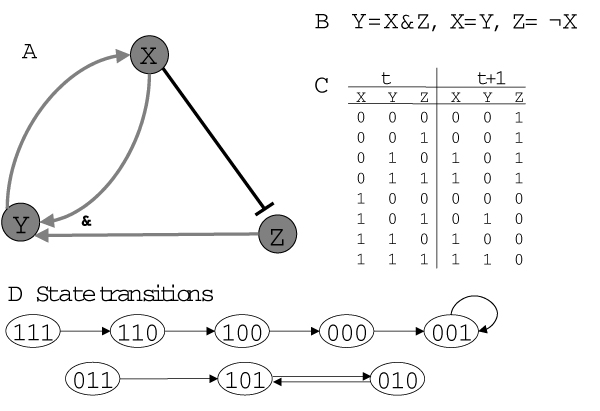
\includegraphics[width=0.7\textwidth]{BooleanNetwork.png}
    \caption[Boolean Network]{4 ways of representing a Boolean Network: A. regulatory network, B. Boolean functions, C. transition interpretations, D. State transition graph}
    \label{fig:booleannetwork}
\end{figure}

The representation of Boolean functions is concise but does not indicate intuitively the state change between moment $t$ and $t+1$.
Transition interpretations and state transition graph are straightforward but there are two drawbacks: 
\begin{itemize}
    \item their needed memory increases exponentially
    \item they are not equivalent to Boolean functions
\end{itemize}
One set of transition interpretations or one state transition graph could correspond to multiple set of Boolean functions.

Also, BN can be translated to Normal Logic Program (NLP) \cite{inoue2011logic} for a more dynamical representation and also for applying SAT techniques in the computation of point attractors of both synchronous and asynchronous semantics.

%\subsection{Normal Logic Program (NLP)}

\subsection{Process Hitting (PH)}
If one wants to describes the dynamics more finely with reasonable memory use, Process Hitting (PH) framework is a good choice, which introduced by Paulev\'e \textit{et al.} \cite{pauleve2011}.

PH is inspired by $\pi$-calculus, which expresses the communication between canals. 
In PH, the corresponding meaning becomes the interaction between different components.
Process Hitting is an asynchronous automata network, i.e. allowing at most one transition fired simultaneously. 
PH is more expressive than Asynchronous Thomas' model \cite{thomas1978} or Asynchronous BN. 
Actions in Process Hitting are more capable of describing various transitions than Boolean functions or attractors as it specifies the regulating and regulated components and their quantitative levels.
Also it expresses explicitly cooperations between several components and stochastic features using $\pi$-calculus which are not detailed in this report \cite{pauleve2014}.

Moreover, in order to define efficient analysis techniques that avoid to build the whole state space of the model causing state space explosion (in Thomas' model and Boolean network), various abstract structures have been introduced, and one of them is graph of causality, which allows a reasoning of the reachability of local states instead of traverse of global states.

It gathers a finite number of concurrent processes grouped into a finite set of sorts. A process belongs to one and only one sort and is denoted as $a_i$ where $a$ is the sort and $i$ the identifier of the process within the sort $a$.
At any time, only one process of each sort is present, forming a state of the PH.

\begin{definition}[Process Hitting (PH)]
A $PH$ consists of a triplet $(\Sigma, L, H)$:
\begin{itemize}
    \item $\Sigma=\{a,b,...\}$ is the finite set of sorts
    \item $L=\prod_{a\in\Sigma}{L_a}$ is the set of states with $L_a=\{a_0,...a_{l_a}\}$ the finite and countable set of processes of sort $a\in\Sigma$ and $l_a$ a positive integer with: $a\neq b\to \forall(a_i,b_j)\in L_a\times L_b,a_i\neq b_j$
    \item $H=\{h=a_i\to b_j\Rsh b_k\mid(a,b)\in\Sigma^2, (a_i,b_j,b_k)\in L_a\times L_b\times L_b,b_j\neq b_k, a=b\to a_i=b_j\}$ is the finite set of actions, which defines the regulations and dynamics of the PH: $a_i, b_j, b_k$ are denoted $hitter(h)$, $target(h)$ and $bounce(h)$ respectively of the action $h=a_i\to b_j\Rsh b_k$.
\end{itemize}
\end{definition}

\begin{figure}[ht]
\centering
\begin{tikzpicture}%[font=\scriptsize]
%\path[use as bounding box] (0,-1) rectangle (4,4);
%{left, right, top, bottom}
\TSort{(0,0)}{a}{2}{l}
\TSort{(3,0)}{b}{3}{l}
\TSort{(6,0)}{d}{3}{r}
\TSort{(2,-2)}{c}{2}{b}
\THit{a_1}{}{b_1}{.west}{b_0}
\THit{a_0}{}{c_0}{.north}{c_1}
\THit{b_1}{}{a_0}{.east}{a_1}
\THit{c_1}{out=120,in=255}{b_0}{.west}{b_1}
\THit{b_0}{}{d_0}{.west}{d_1}
\THit{b_1}{}{d_1}{.west}{d_2}
\THit{b_2}{distance=120pt,out=30,in=40}{d_0}{.east}{d_2}
\THit{d_1}{}{b_0}{.north east}{b_2}
\THit{c_1}{bend right=80pt,distance=80pt}{d_1}{.east}{d_0}

\path[bounce,bend right]
\TBounce{b_1}{}{b_0}{.north}
\TBounce{a_0}{}{a_1}{.south}
\TBounce{d_0}{bend right=50pt,distance=40pt}{d_2}{.south}
\TBounce{b_0}{}{b_2}{.south}
;
\path[bounce,bend left]
\TBounce{d_0}{}{d_1}{.south}
\TBounce{b_0}{}{b_1}{.south}
\TBounce{c_0}{}{c_1}{.west}
\TBounce{d_1}{}{d_2}{.south}
\TBounce{d_1}{}{d_0}{.north}
;
\path[bounce,bend left]
;
\TState{a_1,b_0,c_0,d_1}
\end{tikzpicture}
\caption[Process Hitting]{A PH with initial state $\langle a_1,b_0,c_0,d_1\rangle$.
Full arrows are regulations while dashed arrows are transitions, e.g. $a_0\to c_0\Rsh c_1$  means that $a$ at level $0$ can make $c$ transit from level $0$ to $1$.}\label{fig:PH}
\end{figure}

One drawback of PH: 

\begin{itemize}
    \item Cannot encode correctly the conjunctions in Boolean functions like $f(a)=b\land c$.
\end{itemize}

To overcome this drawback, we need to introduce a cooperative sort $bc$ to represent the conjunction of $b$ and $c$, with 8 actions $b_0\to bc_{10}\Rsh bc_{00}$, $b_0\to bc_{11}\Rsh bc_{01}$, $b_1\to bc_{00}\Rsh bc_{10}$, $b_1\to bc_{01}\Rsh bc_{11}$, $c_0\to bc_{01}\Rsh bc_{00}$, $c_0\to bc_{11}\Rsh bc_{10}$, $c_1\to bc_{00}\Rsh bc_{01}$, $c_0\to bc_{10}\Rsh bc_{11}$.

However, the size of this representation grows exponentially with the size of the conjunction and the behavior of cooperative sorts are not equivalent to that of BN. 
Also, this encoding introduces extra reactions, producing a temporal shift between the presence of the reactants and the playability of the reaction.

\subsection{Asynchronous Automata Network (AAN)}
Facing the drawback of PH, i.e. only cooperative sorts can encode multimolecular reactions, Asynchronous Automata Network (AAN) is introduced by by Folschette \textit{et al.} \cite{folschette2015}.
AAN allows one to naturally model cooperations by defining several requisites for a transition.
Moreover, such automata networks are still compatible with the notion of priority, that can also be used to model different reaction rates in the model.
AAN (and, a fortiori, their restriction, the PH framework) can be considered as a subset of Communicating Finite State Machines or safe Petri Nets \cite{pauleve2012process}.

Basically there is one difference between PH and AAN. 
In AAN, the definition of $H$ becomes

\begin{itemize}
    \item $H=\{A\to b_j\Rsh b_k\mid b\in \Sigma \land (b_j,b_k)\in L_b\times L_b\land b_j\neq b_k\land \forall a \in \Sigma,\ |a\cap L_a|\leq 1 \land A\cap L_b=\varnothing\}$ is the finite set of actions, which defines the regulations and dynamics of the AAN: $A, b_j, b_k$ are denoted $hitter(h)$, $target(h)$ and $bounce(h)$ respectively of the action $h=A\to b_j\Rsh b_k$.
\end{itemize}



\section{Model Checking}
Model Checking is an automatic verification technique for large state transition systems and was independently developed by Clarke and Emerson \cite{clarke1981design} and by Queille and Sifakis \cite{queille1982specification} in the early 1980s. It was originally developed for reasoning about finite-state concurrent systems.
Typically, a model checker has three basic components: a modeling formalism adopted to encode a state machine representing the system to be verified, a specification language based on Temporal Logic, and a verification algorithm \cite{clarke20142} which employs an exhaustive searching of the entire state space to determine whether the specification holds or not.

In this thesis we focus on reachability (\textbf{EF} in Temporal Logic) as most temporal properties can be reduced to reachability problems due to the expresiveness of hybrid modeling frameworks.

\subsection{Exact Model Checkers}
At first, Model Checking was done by the search in the state transition graphs, which are encoded in adjacent lists \cite{clarke1981design}.
This representation however requires a memory growing exponentially with the number of components.
To avoid such explicit representation, state transition graphs were replaced by Boolean formulas.
OBDD (Ordinary Binary Decision Diagram) based Model Checkers were developed, having reached $10_{120}$ states, e.g.
SMV \cite{mcmillan1993symbolic}, NuSMV \cite{cimatti2000nusmv}, and VIS \cite{brayton1996vis}.
However, the performance is still not enough to analyze problems in systems biology (time-memory out), which is illustrated in Chapter \ref{chap:test}.  

\subsection{Static Analyzers}
Model Checkers are widely applied to hardware and software.
Especially when applied to software, algorithmic verification techniques have
to deal with software’s infinite state space, requiring abstraction techniques to make problems tractable.
SPIN \cite{holzmann1997model} and Goanna \cite{fehnker2006goanna} are designed as source code analyzers, by verifying a set of over-approximative conditions, they managed to check the safety/liveness properties of a program or whether certain program behaves as expected. 
However, the static code analyzers only determines run-time properties of programs by examining the code structure, which may produce false-positive and false-negative results \cite{vorobyov2010comparing}.

Inspired by these ideas, Pint \cite{Pint} takes the initiative to apply pure static analysis, combine over-approximation and under-approximation to squeeze the state space try to solve the original reachability problem of a PH or an AAN.
Similarly, due to the approximations, the result of Pint is not necessarily conclusive \cite{folschette2015}.

\begin{figure}
    \centering
    \begin{tikzpicture}[scale=0.8]
  \coordinate (c) at (0,0);
  \draw[thick,blue,rounded corners=1mm,dashed] (c) \irregularcircle{3cm}{3mm};
  %\draw[blue] (-1.2,-1.2) -- (1.2,-1.2) -- (1.2,1.2) -- (-1.2,1.2) -- (-1.2,-1.2);
  \draw[thick,purple] (-2.5,-1.2) -- (2.5,-1.2) -- (2.5,1.2) -- (-2.5,1.2) -- (-2.5,-1.2);
  \draw[thick,purple] (-7,-3.5) -- (3.5,-3.5) -- (3.5,3.5) -- (-7,3.5) -- (-7,-3.5);
  \node (under) at (0,0) {Under-approximation};
  \node [text width=3cm] (over) at (-4.8,0) {Over-\\approximation};
  \node (real) at (0,2) {Real dynamics};
\end{tikzpicture}
    \caption[Static analysis]{Schema of real dynamics and over-approximation and under-approximation}
    \label{fig:vennDiagram}
\end{figure}

\subsection{Reachability Problem}
In the domain of model checking, reachability has been of great interest for over 30 years \cite{clarke2008birth,clarke20142}. 
Various modeling frameworks and semantics in bioinformatics have been studied: Boolean network \cite{akutsu2007control}, Petri nets \cite{mayr1984,esparza1998}, timed-automata \cite{Daws1998,wozna2003}. 
These approaches rely on global search and thus face state explosion problem as the state space grows exponentially with the number of variables. 
In \cite{peterson1977petri}, it has been shown that the reachability problem of Petri net is exponential time-hard and exponential space-hard, and this conclusion does not change even under some specific conditions \cite{esparza1998}. 
For 1-safe Petri nets, the complexity of reachability analysis is generally PSPACE-complete \cite{cheng1995complexity}.
Li \textit{et al.} \cite{li2012reachability,li2014stability} investigated theoretically the stability, the controllability and the reachability of Switched Boolean Networks, but their method remains computationally expensive;
Saadatpour \textit{et al.} \cite{saadatpour2010attractor} researched only the reachability of fixed points.

To tackle the complexity issue, symbolic model checking \cite{burch1992symbolic} based on OBDDs and SAT-solvers (satisfiability) \cite{abdulla2000symbolic} have been studied over years, but still fail to analyze big biological systems with more than $1000$ variables. 
Bounded Model Checking (BMC) \cite{clarke2001bounded} is an efficient approach but generally not complete as its searching depth is limited to a given integer $k$.
\section{Semantics of Modelings}
For different modeling frameworks, even if the components and transitions are defined, the dynamics of the system is not unique. 
Different update schemes lead to different dynamics.
The main difference lies on the relataions of the number of transitions \textit{can} be fired and the number of transitions \textit{will} be fired at given time point $t$.
%\cite{ribeiro2018learning}


\subsection{Synchronicity}
Intuitively, synchronous update scheme implies that every fireable transition is fired simultaneously.
It seems to be deterministic. 
However, when there are multiple fireable transition for one variable, there are multiple possible future states which cannot be fired simultaneously.
\begin{example}
Given an NLP with transitions $c_1\gets a_1$ and $c_2\gets b_1$ and initial state $\langle a_1, b_1, c_0\rangle$, these 2 transitions are in conflict.
Even though the semantics is synchronous, a choice is need to be made between these transitions.
\end{example}

To avoid the conflicts, one possible solution in BN is to clarify the state transition metrics:
for one variable, if it can change its value at the next time point, it cannot keep its current value.

Computationally, one of the benefits of the synchronous model is tractability, while classical state space exploration algorithms fail on asynchronous ones.
For some applications, like the biological ones, asynchronous semantics is said to capture more realistic behaviors: at a given time, a single gene can change its expression level.
This results in a potential combinatorial explosion of the number of reachable states.

\begin{figure}[ht]
%\begin{minipage}[ht]{0.32\textwidth}
\subfigure[0.31\textwidth][Synchronous semantics]{
\begin{tikzpicture}[scale=0.87,line width=1pt]
\draw[->] (0,0) -- (3.5,0);
\draw	[->] (0,0) -- (0,2.5);
\draw[step=1] (0,0) grid (3,2);
\node at (3.5,0)[anchor=north]{\small u};
\node at (0,2.5)[anchor=east]{\small v};
\foreach \x in {0,1,2}
\node at ($(\x,0)+(0.5,0)$)[anchor=north] {\small $\x$};
\foreach \y in {0,1}
\node at ($(0,\y)+(0,0.5)$)[anchor=east] {\small $\y$};
%\node at (1,0)[anchor=north]{$t_{uv}$};
%\node at (2,0)[anchor=north]{$t_{uu}$};
%\node at (0,1)[anchor=east]{$t_{vu}$};
\draw[->] (0.5,1.4) -- (0.5,0.6);
\draw[->] (1.4,1.5) -- (0.6,1.5);
%\draw[dotted,->] (0.6,0.5) -- (2.4,0.5);
\draw[->] (0.6,0.5) -- (2.4,0.5);
%\draw[dashed,->] (1.6,0.6) -- (2.3,1.3);
\draw[->] (1.6,0.6) -- (2.3,1.3);
\draw[->] (2.5,0.6) -- (2.5,1.4);
\draw[->] (2.6,1.4) arc (-90:240:0.25);
\end{tikzpicture}
%\caption{Synchronous dynamics}
%\end{minipage}
}
%\begin{minipage}[ht]{0.32\textwidth}
\subfigure[0.31\textwidth][Asynchronous semantics]{
\begin{tikzpicture}[scale=0.90,line width=1pt]
\draw[->] (0,0) -- (3.5,0);
\draw[->] (0,0) -- (0,2.5);
\draw[step=1] (0,0) grid (3,2);
\node at (3.5,0)[anchor=north]{\small u};
\node at (0,2.5)[anchor=east]{\small v};
\foreach \x in {0,1,2}
\node at ($(\x,0)+(0.5,0)$)[anchor=north] {\small $\x$};
\foreach \y in {0,1}
\node at ($(0,\y)+(0,0.5)$)[anchor=east] {\small $\y$};
%\node at (1,0)[anchor=north]{$t_{uv}$};
%\node at (2,0)[anchor=north]{$t_{uu}$};
%\node at (0,1)[anchor=east]{$t_{vu}$};
\draw[->] (0.5,1.4) -- (0.5,0.6);
\draw[->] (1.4,1.5) -- (0.6,1.5);
\draw[->] (0.6,0.5) -- (1.4,0.5);
\draw[->] (1.6,0.5) -- (2.4,0.5);
\draw[->] (1.5,0.6) -- (1.5,1.4);
\draw[->] (2.5,0.6) -- (2.5,1.4);
\draw[->] (2.6,1.4) arc (-90:240:0.25);
\end{tikzpicture}
%\caption{Asynchronous dynamics}
%\end{minipage}
}
%\begin{minipage}[ht]{0.32\textwidth}
\subfigure[0.31\textwidth][General semantics]{
\begin{tikzpicture}[scale=0.87,line width=1pt]
\draw[->] (0,0) -- (3.5,0);
\draw[->] (0,0) -- (0,2.5);
\draw[step=1] (0,0) grid (3,2);
\node at (3.5,0)[anchor=north]{\small u};
\node at (0,2.5)[anchor=east]{\small v};
\foreach \x in {0,1,2}
\node at ($(\x,0)+(0.5,0)$)[anchor=north] {\small $\x$};
\foreach \y in {0,1}
\node at ($(0,\y)+(0,0.5)$)[anchor=east] {\small $\y$};
%\node at (1,0)[anchor=north]{$t_{uv}$};
%\node at (2,0)[anchor=north]{$t_{uu}$};
%\node at (0,1)[anchor=east]{$t_{vu}$};
\draw[->] (0.5,1.4) -- (0.5,0.6);
\draw[->] (1.4,1.5) -- (0.6,1.5);
\draw[->] (0.6,0.5) -- (1.4,0.5);
\draw[->] (1.6,0.5) -- (2.4,0.5);
\draw[->] (1.5,0.6) -- (1.5,1.4);
\draw[->] (2.5,0.6) -- (2.5,1.4);
\draw[->] (2.6,1.4) arc (-90:240:0.25);
\draw[->] (0.4,0.5) .. controls (1.5,0) .. (2.6,0.5);
\draw[->] (1.6,0.6) -- (2.3,1.3);
\end{tikzpicture}
%\caption{General dynamics}
%\end{minipage}
}
\caption[Update schemes]{State transition graphs of different updating schemes}
\end{figure}
\subsection{Asynchronicity}
In systems biology, however, the asynchronous semantics is widely used to model biological systems because it is closer to real biological phenomena than synchronous one.
Given BN with $n$ variables, from a certain state, there are at most $n$ future states, after $t$ step of evolution, there are O$(n^t)$ possible branches which leads to state space explosion problem.
Due to the complexity, there are less study on analysis of dynamic properties than the synchronous one.
\begin{figure}
    \centering
    \begin{tikzpicture}[scale=0.68]%[scale=0.68]
    \begin{axis}[domain=0:2*pi,legend pos=north east]
    %\addplot[samples=12,mark=x,color=red] {sin(deg(x))}; 
    %\addplot[samples=12,mark=*,color=blue] {cos(deg(x))}; 
    \addplot[mark=none,color=blue] {sin(deg(x))}; 
    \addplot[mark=none,color=red] {cos(deg(x))}; 
    \addplot[mark=none,color=black]{0.5};
    %\addplot[mark=square,color=black] {0*deg(x)};
    \addplot[only marks,color=black] coordinates {
        (0,0)
        (0.5*pi,0)
        (pi,0)
        (1.5*pi,0)
        (2*pi,0)
    };
    \legend{$x=\sin(t)$,$y=\cos(t)$}
    \end{axis}
\end{tikzpicture}
\begin{tikzpicture}[scale=0.68]
    \begin{axis}[domain=0:2*pi,legend pos=north east]
    \addplot[mark=none,color=blue] {sin(deg(x))}; 
    \addplot[mark=none,color=red] {cos(deg(x))}; 
    \addplot[mark=none,color=black]{0.5};
    \addplot[only marks,color=black] coordinates {
        (pi/6,0.5)
        (pi/3,0.5)
        (5*pi/6,0.5)
        (5*pi/3,0.5)
       % (0,0)
       % (0.5*pi,0)
       % (pi,0)
       % (1.5*pi,0)
       % (2*pi,0)
    };
    \legend{$x=\sin(t)$,$y=\cos(t)$}
    \end{axis}
\end{tikzpicture}

    \caption[Discretization]{Adapted version of discretization to asynchronous systems}
    \label{fig:my_label}
\end{figure}

This PhD thesis focuses on the study of reachability of asynchronous modeling frameworks.
\subsection{General Semantics}
General semantics is even more complex than asynchronous semantics.
Given BN and a current state, if there are $m$ variables which may change their value at the next time point, there will be $2^m$ possibilities of the next state.
The benchmark part of \cite{ribeiro2018learning} shows the complexity of general semantics, where the model inference fails with 12 components in the model. 
\begin{table}[ht]
    \centering
    \begin{tabular}{c|c|c}
            &transitions can be fired&transitions will be fired\\
            \hline
         Synchronous & \multirow{3}{*}{$n$} & $m$, at most $n$\\\cline{1-1} \cline{3-3}
            
         Asynchronous & & $\min(1,n)$\\ \cline{1-1} \cline{3-3}
            
         General &  & $[0,n]$
    \end{tabular}
    \caption[Update schemes]{Numbers of fireable transitions in different updating scheme, where $m$ stands for the number of influenced variables}
    \label{tab:semantics}
\end{table}

\section{Resum\'e}

\chapter{Refined Reachability Analysis \textit{via} Heuristics}\label{chap:refinement}
\begin{mybox}
Several modeling frameworks and model checking techniques are introduced in Chapter \ref{chap:stateOfTheArt}.
We noticed that even though there exist already exact model checkers and static analyzers for reachability problems, they are not sufficient.
Exact model checkers face always the state space explosion problem when analyzing large models (of about 50 variables);
Static analyzer PINT, designed for Process Hitting/Automata Network is however, theoretically inconclusive, i.e. not able to provide a global solution to arbitrary input.
This chapter is going to deepen into the reachability problem \textit{via} the following steps:

\begin{itemize}
    \item Why the inconclusiveness problem rises
    \item What are the problematic structures
    \item How to deal with such structures
\end{itemize}

As a result, we try to recover the consequence of the lost information due to non-exhaustive search of static analysis and construct a more close approximation of the real dynamics in order to gain a better conclusiveness.
\end{mybox}

In this chapter, we are going to formally define the main modeling framework studied in this thesis, Asynchronous Binary Automata Network (ABAN) and its related static analyzer, Simplified Local Causality Graph (SLCG).
These two new definitions based on the one of Automata Network in order to adapt to our new reachability analyzers.

Also, to deal with the inconclusiveness problem persisting in previous work \cite{folschette2015}, we propose at first doing some preprocessings by simplifying the topology of the models in order to try to remove the parts leading to inconclusiveness.
Then we will introduce two new analyzers (PermReach and ASPReach) based on over-approximation.
They perform different heuristics, trying to avoid most of the inconclusiveness due to pure static analysis.

\section{Background}
Reachability problem on formal models is a critical challenge where both validation problems (whether the model satisfies the \textit{a priori} knowledge) and prediction problems (properties to be discovered) meet. 
From a formal point of view, numerous biological properties in computational models can be transformed to reachability properties. 
For example, the reachability of state 0/1 of a variable could represent the activation/inhibition of certain gene or synthesis of a protein, while initial state could represent initial observation in an experiment.
If the reachability of a certain state contradicts with \textit{a priori} knowledge, one can modify the model and/or design a new experiment to verify whether there are erroneous information in the \textit{a priori} knowledge or imprecision in the former observations.
Also, reachability analysis is of help to medicine design: for example if one wants to prevent the carcinogenesis of a cell (target state), one possible solution is to find the critical pathways towards the target state and design a medicine to cut them in order to keep the cell healthy.

To tackle the complexity issue, symbolic model checking \cite{burch1992symbolic} based on ordered binary decision diagrams (OBDDs) \cite{hardin1997new} and that based on SAT-solvers (satisfiability) \cite{abdulla2000symbolic} have been studied over years, but still fail to analyze big biological systems with more than $1000$ variables. 
Bounded Model Checking (BMC) \cite{clarke2001bounded} is a state-of-the-art approach, it is efficient but generally not complete as its searching depth is limited to a given integer $k$.
One has no idea whether there exists a solution beyond step $k$ or not.

Beside these approaches, abstraction is an efficient strategy to deal with such models of big scale. 
It aims at approximating the model while keeping the most important parts influencing the reachability.
Abstract approaches often have better time-memory performance but with a loss of information. 
They solve usually a simplified version of the original model, i.e. the results from these approaches are not necessarily compatible with all the properties of the original model.
While studying reachability problems, the system dynamics is abstracted to static causalities between states and transitions.

However, like BMC, abstract approaches do not solve all the instances.
In fact, they solve a simplified version instead of the original reachability problem.
If the result of the simplified version is not sufficient to imply the one of the original problem, abstract approaches fail (inconclusive).
In the following, we are going to formally define the reachability problem and discuss what are the causes of the inconclusiveness and how to solve them. 

\section{Asynchronous Binary Automata Network}
In \cite{folschette2015}, Paulev\'e \textit{et al.} have worked on the modeling of concurrent systems by Asynchronous Automata Network (AAN) and they invented Local causality graph (LCG) \cite{pauleve2017reduction,folschette2015,pauleve2011} to analyze the reachability of AAN.
This interpretation drastically reduces the searching state-space thus avoids costly global search \cite{pauleve2012}. 
However, this pure static analysis is not complete as there are inconclusive cases which can not be decided reachable or not.
LCG can only conclude with the following two constraints:

\begin{itemize}
    \item With no cycles (Section \ref{sec:cycles})
    \item With no \textbf{AND gates} (Section \ref{sec:conclusiveness})
\end{itemize}

We are thus going to refine the reachability analysis to deal with more instances.
To attack the inconclusiveness problem, we have designed a new discrete modeling framework for concurrent systems \cite{chai2018heuristic}: Asynchronous Binary Automata Network (ABAN).
\textbf{WHY} In ABAN, we adapted LCG to SLCG (Simplified LCG) to address reachability problem.
This approach refers to a static abstraction of the reachability (with an over-approximation of the real dynamics).
Under ABAN, SLCG is more prone to conclude than LCG under AAN (Section \ref{sec:SLCG}).

\subsection{Definitions}
\begin{definition}[ABAN]\label{def:ABAN}
An ABAN is a triplet $AB = (\Sigma,L,T)$, where:
\begin{itemize}
\item $\Sigma\triangleq\{a,b,\ldots\}$ is the finite set of automata with every component having a Boolean state;
\item $LS\triangleq \underset{a\in \Sigma}{\cup} \{a_0,a_1\}$ is the set of all \textit{local states}, $L\triangleq \underset{a\in \Sigma'}{\times} \{a_0,a_1\}$ is the set of \textit{joint states} where $\Sigma'\subseteq\Sigma$. Particularly, if $\Sigma'=\Sigma$, $L$ is the set of \textit{global states}. 
\item $T\triangleq \{A\rightarrow b_i\mid b\in \Sigma \land A\in L\}$ is the set of transitions.
For transition $tr=A\to b_i$, $A$ (called head, noted $head(tr)$) is the set of required state(s), which allows to flip $b_{1-i}$ to $b_i$ (called body, noted $body(tr)$). In other words, transition $tr$ is said fireable iff $A\subseteq s$, where $s$ is the current global state. 
\end{itemize}
\end{definition}

\textbf{Remark:} In AAN or PH, the transitions (or called actions) are noted $A\rightarrow b_i\Rsh b_j$ to express ``automaton $b$ changes its value from $i$ to $j$ under condition $A$''.
However, the states in ABAN are all binary, the transition can only be realized from $0$ to $1$ or conversely.
Thus we omit the state before transition while avoiding ambiguity.
It might also be noted the notation $A\rightarrow b_i$ resembles the equivalent notation in Logic Program (LP): $b_i \leftarrow A$.

Also, the notions of different states are \textit{crucial} in this thesis.
A \textit{local state} represents the state of one automaton, \textit{e.g.} $a_1$ means automaton $a$ is at level $1$.
A \textit{joint state} represents the state of a set of automata, \textit{e.g.} $\langle a_1, b_0\rangle$ means automaton $a$ is at level $1$ and automaton $b$ is at level $0$.
In fact, when we take all the automata in the system as the set of automata, the corresponding \textit{joint state} becomes the state of the whole system, which is the global state, \textit{e.g.} given $\Sigma =\{a,b,c\}$, $\langle a_0, b_1,c_0 \rangle$ shows the state of \textit{all} the automata.
To conclude, joint state is the most general case, when $|\Sigma'|=1$, it becomes a local state;
when $\Sigma'=\Sigma$, it becomes a global state.

\begin{definition}[Dynamics]
    From current global state $s$, the global state after firing transition $tr=A\to b_j$ is denoted $s \cdot tr = s \setminus \{b_i\} \cup \{b_j\}, b_i \in s$.
    The state of a certain automaton $a$ is noted $(s\cdot tr)[a]$.
\end{definition}

The definition of dynamics allows one to describe how the system state interacts with the transitions. 
Moreover, to describe the evolution in an ABAN, we use the notion of trajectory.

\begin{definition}[Trajectory]
Given an ABAN $AB = (\Sigma,L,T)$ and a global initial state $\alpha\in L$, a trajectory $t$ from $\alpha$ is a sequence of transitions $t=tr_1::\cdots :: tr_i::\cdots ::tr_n$ with $tr_i\in T$ and each $tr_i$ is fireable in $(\alpha \cdot tr_1 \cdot \ldots \cdot tr_{i-1})$.
From $\alpha$, the global state after firing all transitions of $t$ is $(\alpha \cdot tr_1 \cdot \ldots \cdot tr_n)$, denoted $\alpha \cdot t$.
\end{definition}

A trajectory describe the historical evolution of the system or one possible future evolution by recording the fired transitions. 
An alternative is to record the state changes using state sequence:

\begin{definition}[State sequence]
Given an ABAN $AB = (\Sigma,L,T)$ and a global initial state $\alpha\in L$ and trajectory $t$, the state sequence $seq=s_1::\cdots :: s_i::\cdots ::s_n$ with $s_i\in LS$ is formed by the updated local states during the trajectory $t$.
\end{definition}

Thanks to asynchronicity, at each time step ABAN changes the value of at most one automaton.
That is why we can distinguish the order of state changes, thus form a state sequence.

Example \ref{exABAN} illustrates all the definitions above.
\begin{example}\label{exABAN}
    Figure \ref{fig:exampleABAN} shows an ABAN of 5 automata $a,b,c,d,e$, with the set of transitions $T=\{\acm{b_1,c_1}{a_0}{a_1},\acm{e_1}{a_0}{a_1},\acm{d_0}{b_0}{b_1},\acm{d_1}{c_0}{c_1},\acm{b_1}{d_0}{d_1}\}$ and the initial state $\alpha=\langle a_0,b_0,c_0,d_0,e_0\rangle$.
    A possible trajectory from $\alpha$ is $t=\acm{d_0}{b_0}{b_1}::\acm{b_1}{d_0}{d_1}::\acm{d_1}{c_0}{c_1}::\acm{b_1,c_1}{a_0}{a_1}$.
    After firing the transitions in trajectory $t$, the global state becomes $\Omega=s\cdot t=\langle a_1,b_1,c_1,d_1,e_0\rangle$, and the local state of $a$ is $(\alpha\cdot t)[a]=a_1$. 
    The corresponding state sequence is $seq=b_1::d_1::c_1::a_1$.
\end{example}

\begin{figure}[ht]
\centering
\begin{tikzpicture}[apdotsimple/.style={apdot},scale=0.7, every node/.style={scale=0.8}]
\scriptsize
\TSort{(0,0)}{a}{2}{l}
\TSort{(2,0)}{b}{2}{l}
\TSort{(4,0)}{c}{2}{l}
\TSort{(6,0)}{d}{2}{l}
\TSort{(8,0)}{e}{2}{l}

% with delays
\path[local transitions]

	(a_0) edge node[auto] {\{$b_1, c_1$\}} (a_1)
    (a_0) edge[bend right] node[right] {$\{e_1\}$} (a_1)
	(b_0) edge node[auto] {$\{d_0\}$} (b_1)
	(d_0) edge node[auto] {$\{b_1\}$} (d_1)
	%(c_1) edge node[auto] {$\{b_0\}$, $2$} (c_0)
	(c_0) edge node[auto] {$\{d_1\}$} (c_1)
;

\TState{a_0, b_0, c_0, d_0,e_0}


\end{tikzpicture}

\caption[Example of ABAN]{An example of ABAN}\label{fig:exampleABAN}
\end{figure}

With the definition of trajectory and that of state sequence, we can address reachability problem.

\begin{definition}[Reachability problem]
Given an ABAN, the \textit{joint reachability} $REACH (\alpha,\Omega)$ can be formalized as: joint state $\Omega$ is reachable iff there exists a trajectory $t$ s.t. $\alpha\cdot t=\Omega$.
\textit{Partial reachability} $reach(\alpha,\omega)$ is defined analogously: local state $\omega=a_i$ is reachable iff there exists a trajectory $t$ s.t. $(\alpha\cdot t)[a]=a_i$.
$REACH (\alpha,\Omega)$ and $reach(\alpha,\omega)$ take Boolean values \textbf{True}, \textbf{False} or \textbf{Inconclusive} if it cannot be decided.
\end{definition}

\begin{example}
Taking the same ABAN as in Example \ref{exABAN}, target global state $\Omega=\langle a_1,b_1,c_1,d_1,e_0\rangle$ or target local state $\omega=a_1$ are reachable from the initial state $\alpha$ \textit{via} trajectory $t$ or state sequence $s$, \textit{i.e.} $reach(\alpha,a_1)=\textbf{True}$ and $REACH(\alpha,\Omega)=\textbf{True}$. 
\end{example}

One can define various dynamical properties using reachability, e.g. safety (there exists no trajectory from any initial state to an unwanted state), robustness (there exist trajectories from any initial state to a wanted state).
Moreover, Proposition \ref{def:transformReach} explains the reachability of a joint state even a global state can be transformed to that of a local state.

\begin{proposition}[Transformation of reachability]\label{def:transformReach}
Given ABAN $AB=(\Sigma, L, T)$ and a joint reachability problem $REACH(\alpha,\Omega)$, there exists an ABAN $AB'=(\Sigma', L, T')$ with $\Sigma'=\Sigma\cup\{x\}$ and $T'=T\cup\{\Omega\to x_1\}$ s.t. the local reachability problem in $AB'$ $reach(\alpha', x_1)$ with $\alpha'=\alpha\cup\{x_0\}$ is equivalent to $REACH(\alpha,\Omega)$ in $AB$.
\end{proposition}

\begin{proof}
If $REACH(\alpha,\Omega)=\mathbf{True}$, there must exists a trajectory $t$ satisfying $\alpha\cdot t=\Omega$.
$t$ is consistent with $AB'$ with initial state $\alpha'$ as $AB'$ contains all the elements in $AB$ and $\alpha\subset\alpha'$.
After firing all the transitions in $t$, the global state becomes $\Omega\cup\{x_0\}$, transition $\Omega\to x_1$ is fireable and $x_1$ is reachable from $\alpha'$ \textit{via} $t'=t::\Omega\to x_1$, thus $reach(\alpha', x_1)=\mathbf{True}$. 

If $REACH(\alpha,\Omega)=\mathbf{False}$, there does not exist a trajectory $t$ satisfying $\alpha\cdot t=\Omega$.
In $AB'$, this conclusion remains true as the only added transition $\Omega\to x_1$ is useless in the reachability of $\Omega$.
The only pathway towards $x_1$ is through $\Omega\to x_1$, as $\Omega$ is not reachable, $x_1$ is not reachable, $reach(\alpha', x_1)=\mathbf{False}$.

Similarly, we can prove the global reachability from local one.
\end{proof}

\paragraph{\textbf{One advantage of ABAN}}\label{par:advantage}
Many biological regulatory networks are encoded in Boolean style, \textit{e.g.} in \cite{akutsu2007control,kauffman1969}, because BN is a simple formalism but with strong applicability: discretization in BN is a way to handle the imprecision of \textit{a priori} knowledge on the model.
However BN may be not expressive enough.
If one wants to model the dynamic behavior ``$a\gets$ $1$ at moment $t+1$ if $b=1$ at moment $t$'', the translation is $a(t+1)=b(t)$ in BN.
It means $a$ always follows the evolution of $b$ but with a redundant behavior ``$a\gets 0$ when $b=0$ at moment $t$'' which is not defined in his need.
ABAN models this dynamics as \ac{b_1}{a_0}{a_1} without this redundancy. 
Besides, BNs are transformable to ABANs, and this property makes our approach applicable to a wider domain (Appendix \ref{appendix:trans} Translation between Models).

\subsection{Simplified Local Causality Graph (SLCG)}\label{sec:SLCG}
Paulev\'e \textit{et al.} \cite{pauleve2011} have invented Local Causality Graph (LCG) to analyze reachability problems statically.
LCG abstracts the original problem through an over-approximation (necessary condition) and an under-approximation (sufficient condition).
It is a very efficient tool as there is no global search and all the operations are bounded in polynomial complexity.
However LCG does not guarantee to obtain a result, i.e. some inconclusive instances satisfy the necessary condition but fail sufficient conditions, thus one has no clue about the reachability of these instances.

In this thesis, we make use of the LCG by removing objective nodes needed only in multivalued networks, naming it SLCG (Simplified LCG), then we try to analyze it more deeply to solve inconclusive cases of binary valued systems.
In fact, Didier \textit{et al.} \cite{didier2011mapping} have shown a technique to transform multivalued networks to Boolean networks, which broadened the applicability to multivalued networks.

SLCG is aimed at studying the reachability of a target state while given an ABAN and a global initial state.
SLCG is a goal-oriented method.
It starts with the target state $\omega$, look for transitions reaching the target state, then replace $\omega$ with the bodies of these transitions.
If the current target state is included in the initial state, we find the causal path from the initial state towards $\omega$, otherwise we continue the process, until we reach the initial state or local states we have already traversed.
This process terminates because the local states are finite, of size $O(n)$, where $n$ is the number of automata.
In the worst case, SLCG contains all the local states of the ABAN.

\begin{definition}[Over-approximate SLCG]\label{defSLCG}
Given an ABAN $AB = (\Sigma,L,T)$, a global initial state $\alpha$ and a target local state $\omega$, SLCG $l= (V_{\mathrm{state}},V_{\mathrm{solution}},E)$ is the smallest recursive structure with $E \subseteq (V_{\mathrm{state}}\times V_{\mathrm{solution}})\cap (V_{\mathrm{solution}}\times V_{\mathrm{state}})$ which satisfies:
\begin{eqnarray*}
    \omega&\in& V_{\mathrm{state}} \\
    a_i\in V_{\mathrm{state}} &\Leftrightarrow& \{ (a_i, sol_{a_i}\mid head(sol_{a_i})=a_i)\}\subseteq E \\
    sol_{a_i}\in V_{\mathrm{solution}}&\Leftrightarrow& \{ (sol_{a_i},\mathbf{V}(sol_{a_i}))| \mathbf{V}(sol_{a_i})=\varnothing \text{ \rm if } a_i\in \alpha,\\
    &&\text{ \rm else }\mathbf{V}(sol_{a_i})\in body(sol_{a_i}) \}\subseteq E
\end{eqnarray*}
where $V_{\mathrm{state}}\subseteq LS$ is a set of local states, $V_{\mathrm{solution}}\subseteq T$ is the a of solutions and $\mathbf{V}(sol_{a_i})$ is the set of required local states of $sol_{a_i}$.
\end{definition}

It is worth noticing that every state node in $V_{\mathrm{state}}$ forms an \textbf{OR gate} as a local state $a$ is reachable if there exists one fireable transition with body $a$.
Similarly, every solution node in $V_{\mathrm{solution}}$ forms an \textbf{AND gate} as a transition is fireable only if all the local states in its head are reachable.

\begin{remark}
Original LCGs consist of three kinds of nodes: \textbf{state nodes} corresponding to the local states of automata {\rm($V_{\mathrm{state}}$)}, \textbf{objective nodes} corresponding to the state transition paths within one automata {\rm($V_{\mathrm{objective}}$)}, \textbf{solution nodes} corresponding to the transitions to be used for each state transition path {\rm($V_{\mathrm{solution}}$)}.
However, under the circumstance of ABAN, objective nodes are no longer needed.
Because for one state $a_i$ to be reached, the only possible path is $a_{1-i}\to a_i$ ($0\to1 $ or $1\to 0$).
Unlike multi-valued case, for example, if one wants to reach $a_1$ from $a_0$ (suppose possible states for $a$ are 0,1,2), there are in fact infinite possibile paths: $0\to 1,\ 0\to 2 \to 1,\ 0 \to 2 \to 0 \to 1,\ \ldots$
This simplification in fact reduces the searching space and reinforces the conclusiveness.
\end{remark}

\begin{example}
    Figure \ref{LCGexample} shows the SLCG for analyzing $reach(a_1)$ in Example \ref{exABAN}.
    There are two pathways from $a_1$ to $\alpha$: $a_1\to \circ\to b_1\to \circ\to d_0$ and $a_1\to \circ\to c_1\to \circ\to d_1\to \circ\to b_1\to \circ \to d_0$.
    %$a_1\to \acm{b_1,c_1}{a_0}{a_1}\to b_1\to \acm{d_0}{b_0}{b_1}\to d_0$ and $a_1\to \acm{b_1,c_1}{a_0}{a_1}\to c_1\to \acm{d_1}{c_0}{c_1}\to d_1\to \acm{b_1}{d_0}{d_1}\to b_1\to \acm{d_0}{b_0}{b_1}\to d_0$.
    \begin{figure}[ht]
        \centering
        \begin{tikzpicture}[aS,scale=0.7, every node/.style={scale=0.7}]  
  	
  	\startl{a_1};
    \node[Asol,left of=a_1] (a_1s1){};
    \node[Aproc,left of=a_1s1] (e_1){$e_1$};
    \path 
    (a_1s1) edge (e_1)
    (a_1) edge (a_1s1)
    ; 
  	\specl{above}{a_1}{b_1};
  	\link{b_1}{d_0};
  	\edl{d_0};
  	\specl{below}{a_1}{c_1};
	\link{c_1}{d_1};
    \path (d_1s) edge (b_1);
    \end{tikzpicture}

        \caption[SLCG]{Visualization of SLCG, with the squares representing local states and small circles representing solution nodes.
        $\varnothing$ signifies that there is no need to link any transitions, i.e the former state $d_0$ is in the initial state.}
        \label{LCGexample}
    \end{figure}
\end{example}

Algorithm \ref{AlgConstructLCG} in Appendix describes how to construct an SLCG from an ABAN $AB = (\Sigma,L,T)$.
Starting from  a given target local state $\omega$, one can find all the transitions $T_s\subseteq T$ reaching $\omega$ and add edges $\omega \to T_s$.
Then we find all the heads $A$ of $T_s$ and add edges $T_s \to A$ and replace $Ls$ with $A$ (recursion).
Finally, we update the structure until $Ls\subseteq \alpha$ or there is no transition with body in $Ls$.

Intuitively, when the recursive construction is complete, SLCG is in fact a digraph with state nodes $V_{\mathrm{state}}$ and solution nodes $V_{\mathrm{solution}}$. 
$E$ consists of the edges between local state nodes and solution nodes. 
To access certain local states, at least one of its successor solutions (corresponding transitions from solution nodes) needs to be fired; to make one solution node fireable, all of its successor local states need to be satisfied. 
A recursive reasoning of reachability tries to explore a pathway.
It begins with a state node representing target local state, goes through $a_i\to sol_{a_i}\to b_j \cdots$ and ends with the initial state (possibly reachable) or a local state without successor solution node (unreachable). 

With SLCG, it is easy to verify whether their are potential pathways from the target state $\omega$ to the initial state $\alpha$ as the causal relations with form $state\to transition$ and $transion\to state$ are indicated on the graph.
If there does not exist such a pathway, one can ensure that $\omega$ is not reachable from $\alpha$.

Pseudo-reachability is a procedure computing the existence of such pathway by confirming whether the transitions are enough (in causal sense) for $\omega$ to be reachable without considering the system evolution.
However, pseudo-reachability is named ``pseudo'' because it is only an over-approximation of the reachability, i.e. it verifies a necessary condition of the reachability.

\begin{definition}[Pseudo-reachability]\label{defPseudoReach}
Given an SLCG $l=(V_{\mathrm{state}},V_{\mathrm{solution}},E)$ with global initial state $\alpha$, the pseudo-reachability of node $v\in V_{\mathrm{state}}$ is defined as
\begin{equation}
\nonumber
    reach'(\alpha,v)=
    \begin{cases}
        \mathrm{\bf True} & {\rm if\ } v\in \alpha\\
        \mathrm{\bf False} & {\rm if\ } v\not\in \alpha\ {\rm and} \not\exists(s,sol) \in E\\
        \bigvee_{(s,sol) \in E} \mathrm{fireable}(sol) & otherwise
        %\bigvee_{(s,sol) \in E}  (\bigwedge_{(sol,s)\in E} reach'(\alpha,s)) & {\rm otherwise}
    \end{cases}
\end{equation}
where $\mathrm{fireable}(sol)=\bigwedge_{(sol,s)\in E} reach'(\alpha,s)$. 

\end{definition}

\subsection{Conclusiveness}\label{sec:conclusiveness}

When pseudo-reachability suggests \textbf{True}, due to its non-equivalence with reachability, we cannot assure the pathway from $\omega$ to $\alpha$ is \textit{dynamically realizable}.
We are going to show several counter-examples as follows:

\begin{example}\label{example:unreach}
    In Figure \ref{fig:limitation}, $reach'(\alpha,c_1)=reach'(\alpha,a_1)\land reach'(\alpha,b_1)=reach'(\alpha,a_0)\land reach'(\alpha,b_0)=\textbf{True}$. Both $a_1$ and $b_1$ are reachable, but they can not be reached simultaneously.
    In such SLCG, there are two branches, $a_1\to b_0$ and $b_1\to a_0$, the automata $a$ and $b$ involve themselves in different branches, the reachability of $a_1$ impedes the reachability of $b_1$ and \textit{vice versa}.
\end{example}

\begin{figure}[ht]
    \centering
    \begin{minipage}{0.4\textwidth}
\centering
\begin{tikzpicture}[apdotsimple/.style={apdot},scale=0.7, every node/.style={scale=0.8}]
\scriptsize
\TSort{(0,0)}{a}{2}{l}
\TSort{(2,0)}{b}{2}{l}
\TSort{(4.5,0)}{c}{2}{l}

% with delays
\path[local transitions]

	(c_0) edge node[auto] {\{$a_1, b_1$\}} (c_1)
	(a_0) edge node[auto] {\{$b_0$\}} (a_1)
	(b_0) edge node[auto] {\{$a_0$\}} (b_1)
;
\TState{a_0, b_0, c_0}
\end{tikzpicture}
\end{minipage}\hfill
\begin{minipage}{0.6\textwidth}
\centering
\begin{tikzpicture}[aS,scale=0.7, every node/.style={scale=0.7}]  
  	
  	\startl{c_1};
  	\specl{above}{c_1}{a_1};
  	\link{a_1}{b_0};
  	\edl{b_0};
  	\specl{below}{c_1}{b_1};
	\link{b_1}{a_0};
  	\edl{a_0};
\end{tikzpicture}
\end{minipage}
    \caption[Limitation of SLCG 1]{$\Sigma=\{a,b,c\}$, $T=\{\acm{b_0}{a_0}{a_1},\ \acm{a_0}{b_0}{b_1},\ \acm{a_1,b_1}{c_0}{c_1}\},\omega=c_1$}
    \label{fig:limitation}
\end{figure}

Also, the recursive reasoning does not terminate if there exists cycles in SLCG. 
While computing the pseudo-reachability, self-dependent structure  $reach'(\alpha,a_i)=\ldots=reach'(\alpha,a_i)$ might appear and cannot be computed by using Definition \ref{defPseudoReach}. 
In Figure \ref{fig:limitation2}, dealing with cycles becomes inevitable.

\begin{figure}[ht]
    \centering
    \begin{tikzpicture}[aS,scale=0.9, every node/.style={scale=0.9}]  
  	
  	\startl{c_1};
  	\specl{above}{c_1}{a_1};
  	\link{a_1}{b_0};
  	\edl{b_0};
  	\specl{below}{c_1}{b_1};
	\link{b_1}{a_0};
  	\edl{a_0};
    \path
    	(a_0s) edge (a_1)
        (b_0s) edge (b_1)
    ;
    \end{tikzpicture}

    \caption[Limitation of SLCG 2]{SLCG with cycles, $\Sigma=\{a,b,c\}$, $T=\{\acm{b_0}{a_0}{a_1},\ \acm{a_0}{b_0}{b_1},\ \acm{a_1,b_1}{c_0}{c_1},\varnothing \to a_0, \varnothing \to b_0\},\omega=c_1$}
    \label{fig:limitation2}
\end{figure}

\section{Preprocessing of Simplified Local Causality Graph}\label{sec:chap3preprocessing}

We have shown some example of inconclusiveness due to cycles and \textbf{AND gates}. 
In this section, we are going to analyze these two special structures and offer two solutions to the inconclusiveness.

\subsection{Detection and Removal of Cycles}\label{sec:cycles}
\begin{definition}[Cycle]
In an SLCG, a cycle is formed by a sequence of nodes linked as follows: $a_i\to \circ \to \cdots \to \circ \to a_i$, where circles stand for solution nodes.
\end{definition}

To identify cycles, we search instead Strongly Connected Components (SCC) of size greater than one.
Because cycles may have intersections but there is no such problem with SCC.
In other words, a SCC contains as many as possible nested cycles which strongly connect to each other.
\cite{tarjan1972} shows that the detection of SCCs can be done in $O (|V|+|E|)$ time, with $|V|$ the number of the vertices and $|E|$ the number of the edges.
SLCG is usually a sparse graph, as in biological systems, the components mostly interact with only a part of the system, hence the out-degree can be considered of $O (1)$ and the detection of SCCs\footnote{Implementation in Python3 by Mario Alviano at \url{https://github.com/alviano/python/blob/master/rewrite_aggregates/scc.py}} can be done in $O(|V|)$, \textit{i.e.} linear time.

\begin{theorem}\label{th:break_cycle}
Given a cycle $x\to \circ \to \cdots \to \circ \to x$ in an SLCG, if there is at most one incoming edge to the cycle, the cycle can be removed.
\end{theorem}

\begin{proof}
If there is no incoming edge, the target state $y$ must be in the cycle. 
The edge $y.pred\to\circ\to y$ can be removed, because the reachability of $y.pred$ requires $y$, but $y$ is the target state, which is never reached before the other local states in the SLCG are reached.
Thus the transition corresponding to this edge is never fired and the edge can be removed.
Similarly, if there is an outside incoming edge $a\to \circ \to x$, $a$ must be the successor of target state $y$ or the target itself, $x.pred\to\circ\to x$ can hence be removed.
\end{proof}

\begin{example}
    \begin{figure}[ht]
        \centering
        \begin{tikzpicture}[->, >=stealth]
\scriptsize
\def \n {6}
\def \radius {1.4cm}
\def \margin {8} % margin in angles, depends on the radius



\node[draw] at ({360/\n * 2}:\radius) (x) {$x$};
\node[draw, circle, minimum size=4pt, inner sep = 0] at ({360/\n * 3}:\radius) {};
\node[draw] at ({360/\n * 4}:\radius) (y) {$y$};
\node[draw, circle, minimum size=4pt, inner sep = 0] at ({360/\n * 5}:\radius) {};
\node[draw] at ({360/\n * 6}:\radius) (z) {$z$};
\node[draw, circle, minimum size=4pt, inner sep = 0] at ({360/\n * 1}:\radius) {};
\foreach \s in {3,...,\n}
{
  
  \draw ({360/\n * (\s - 1)+\margin}:\radius) 
    arc ({360/\n * (\s - 1)+\margin}:{360/\n * (\s)-\margin}:\radius);
}
\foreach \s in {1,2}
{
  
  \draw[dashed] ({360/\n * (\s - 1)+\margin}:\radius) 
    arc ({360/\n * (\s - 1)+\margin}:{360/\n * (\s)-\margin}:\radius);
}
\node[left = 0.8cm of x, draw, circle, minimum size=4pt, inner sep = 0] (sol) {};
\node[left = 0.8cm of sol, draw] (origin) {$a$};
\draw (origin) to [bend left] (sol);
\draw (sol) to [bend left] (x);

\node[right = 0.8cm of z, draw, circle, minimum size=4pt, inner sep = 0] (solz) {};
\node[right = 0.8cm of solz, draw] (ext) {$w$};
\node[right = 0.8cm of ext] (etc) {$\cdots$};
\draw (z) to [bend left] (solz);
\draw (solz) to [bend left] (ext);
\draw (ext) to [bend left] (etc);
\end{tikzpicture}
        \caption[SLCG with cycles]{SLCG $l$ containing cycle $x\to \circ \to y \to \circ \to z\to \circ \to x$}
        \label{cycle1}
    \end{figure}
    
    In Figure \ref{cycle1}, the pseudo-reachability of $a$ in SLCG $l$ is 
    \begin{eqnarray*}
       reach'(\alpha,a)&=&reach'(\alpha,x)=reach'(\alpha,y)=reach'(\alpha,z)    \\
         &=&reach'(\alpha,x)\lor reach'(\alpha,w)
    \end{eqnarray*}
    To reach $x$, we need to reach $z$, but $z$ cannot depend on $x$ as $x$ is already to be reached. 
    Self-dependence appears: $x$ is reachable if $x$ is reachable.
    Thus edge $z\to \circ \to x$ is deleted (dashed line).
\end{example}
Unfortunately, not all cycles are removable via Theorem \ref{th:break_cycle}.

When there are cycles that cannot be deleted according to Theorem \ref{th:break_cycle}, we can apply Theorem \ref{th:break_cycle2}.
It is associated with the decomposition of SLCG in the next section.
The decomposition of SLCG replaces all the \textbf{OR gates} with one of their branches, then the cycles are either broken, either has no outgoing edge which leads to unreachability.
Example \ref{example:cycles} explains the issue.

\begin{theorem}\label{th:break_cycle2}
Given a cycle, if it contains no edge towards outside of the cycle, all the local states in the cycle are unreachable.
\end{theorem}

\begin{proof}
Suppose an arbitrary cycle $C=a_i\to \cdots b_j\to\cdots \to a_i$, with $\to$ an edge in the SLCG.
Note that $reach'(\alpha,a_i)\implies reach'(\alpha,b_j)\implies reach'(\alpha,b_j.next)\implies \cdots\implies reach'(\alpha,a_i)$.
According to the definition of $reach'$, $reach'(\alpha,a)=\mathbf{True}$ only if $\exists c_k\in C$ and $c_k\in \alpha$.
If there exists such $c_k$, $C$ should not exist as the reasoning stops at $c_k$ and does not form a cycle, contradiction.
$reach'(\alpha,a_i)=reach'(\alpha,b_j)=\cdots =\mathbf{False}$.
\end{proof}

    \begin{figure}[ht]
        \centering
        \begin{tikzpicture}
\scriptsize
\def \n {6}
\def \radius {1.4cm}
\def \margin {8} % margin in angles, depends on the radius



\node[draw] at ({360/\n * 2}:\radius) (x) {$x$};
\node[draw, circle, minimum size=4pt, inner sep = 0] at ({360/\n * 3}:\radius) {};
\node[draw] at ({360/\n * 4}:\radius) (y) {$y$};
\node[draw, circle, minimum size=4pt, inner sep = 0] at ({360/\n * 5}:\radius) {};
\node[draw] at ({360/\n * 6}:\radius) (z) {$z$};
\node[draw, circle, minimum size=4pt, inner sep = 0] at ({360/\n * 1}:\radius) {};
\foreach \s in {1,...,\n}
{
  
  \draw[->, >=latex] ({360/\n * (\s - 1)+\margin}:\radius) 
    arc ({360/\n * (\s - 1)+\margin}:{360/\n * (\s)-\margin}:\radius);
}

\node[left = 0.8cm of x, draw, circle, minimum size=4pt, inner sep = 0] (sol) {};
\node[left = 0.8cm of sol, draw] (origin) {$a$};
\draw[->, >=latex] (origin) to [bend left] (sol);
\draw[->, >=latex] (sol) to [bend left] (x);
\node[below = 0.8cm of origin, draw, circle, minimum size=4pt, inner sep = 0] (soly2) {};
\draw[->, >=latex] (origin) to [bend right] (soly2);
\draw[->, >=latex] (soly2) to [bend right] (y);
\draw[->, >=latex] (sol) to [bend right= 45] (z);
\end{tikzpicture}
        \caption[Removal of cycles]{$x,y,z$ all have external links, thus none of the links can be discarded.}
        \label{cycle3}
    \end{figure}

\begin{example}\label{example:cycles}
    In Figure \ref{cycle3}, cycle $C=x\to \circ \to y \to \circ \to z\to \circ \to x$ possesses 3 incoming edges, which is unbreakable according to Theorem \ref{th:break_cycle}.
    But with Theorem \ref{th:break_cycle2}, if \textbf{OR gates} are removed, the cycle can be dealt with.
    At node $a$, there is an \textbf{OR gate} with two branches (filled circles).
    No matter which is branch chosen in the decomposition phase, there is no edge towards cycle $C$.
    $x,y,z$ are all unreachable, hence $a$ is unreachable.
\end{example}

\subsection{Decomposition of SLCG}\label{sec:decomp}

For every \textbf{OR gate}, it has multiple successor transitions (solution nodes) for reaching its corresponding local state.
Fixing the transition choice of all the \textbf{OR gates} is called an \textit{assignment}.
If one wants to discover all the solutions, he needs to traverse all the assignments which is exponential.
To avoid combinatorial explosion, we use a simple heuristic: 
choose randomly one assignment for each trial.
Then, we can construct a new SLCG without \textbf{OR gate}, every state node has exactly one successor solution node, see Figure \ref{fig:heuristics}.

\begin{figure}[ht]
    \centering
    \begin{tikzpicture}[level/.style={sibling distance=70mm/#1},scale=0.5]
\node [circle,draw] (z){$t$}
  child {node [circle,draw,fill=gray] (a) {}
    child {node [circle,draw,fill=gray] (b) {}
      child {node {$\vdots$}
        child {node [circle,draw] (d) {}}
        child {node [circle,draw,fill=gray] (e) {}}
      } 
      child {node {$\vdots$}}
    }
    child {node [circle,draw] (g) {}
      child {node {$\vdots$}}
      child {node (mid) {$\vdots$}}
    }
  }
  child {node [circle,draw] (j) {}
    child {node [circle,draw] (k) {}
      child {node {$\vdots$}}
      child {node {$\vdots$}}
    }
  child {node [circle,draw] (l) {}
    child {node {$\vdots$}}
    child {node (c){$\vdots$}
      child {node [circle,draw] (o) {}}
      child {node [circle,draw] (p) {}
        child [grow=right] {node (q) {} edge from parent[draw=none]
          child [grow=right] {node (q) {} edge from parent[draw=none]
            child [grow=up] {node (r) {} edge from parent[draw=none]
              child [grow=up] {node (s) {} edge from parent[draw=none]
                child [grow=up] {node (t) {} edge from parent[draw=none]
                  child [grow=up] {node (u) {} edge from parent[draw=none]}
                }
              }
            }
            child [grow=down] {node (v) {}edge from parent[draw=none]}
          }
        }
      }
    }
  }
};
\node [right = 2.3cm of e] (point){$\cdots$};
\path (a) -- (j) node [midway] {};
\path (b) -- (g) node [midway] {};
\path (k) -- (l) node [midway] {};
\path (k) -- (g) node [midway] {};
\path (d) -- (e) node [midway] {};
\path (o) -- (p) node [midway] {};
\path (o) -- (e) node (x) [midway] {}
  child [grow=down] {
    node (y) {}
    edge from parent[draw=none]
  };
\path (q) -- (r) node [midway] {};
\path (s) -- (r) node [midway] {};
\path (s) -- (t) node [midway] {};
\path (s) -- (l) node [midway] {};
\path (t) -- (u) node [midway] {};
\path (z) -- (u) node [midway] {};
\path (j) -- (t) node [midway] {};
\path (y) -- (x) node [midway] {};
\path (v) -- (y)
  node (w) [midway] {};
\path (q) -- (v) node [midway] {};
\path (e) -- (x) node [midway] {};
\path (o) -- (x) node [midway] {};
\path (y) -- (w) node [midway] {};
\path (v) -- (w) node [midway] {};
\path (r) -- (c) node [midway] {};
\end{tikzpicture}
    \caption[Random choice on \textbf{OR gates}]{Random choice on \textbf{OR gates}. Descending from the target state, when we encounter an \textbf{OR gate}, we choose randomly one of its branches. Circles filled gray stand for one possible assignment.}
    \label{fig:heuristics}
\end{figure}

\section{Reachability Analysis}
After the preprocessings introduced in the previous section, we can get rid of cycles and \textbf{OR gates}.
The next step is to analyze an SLCG with only \textbf{AND gates}.
We need to find a trajectory reaching all the components of the \textbf{AND gates} simultaneously.
Usually one cannot achieve good conclusiveness and low complexity at the same time, that is why we propose two solutions for different needs of conclusiveness-complexity balance: Reachability via search in permutations (PermReach) which is a partial search and Reachability via Answer Set Programming (ASPReach) which is a exhaustive search.

\subsection{Reachability via Permutations (PermReach)}

Before running into the definitions, we compare Example \ref{example:unreach} and Example \ref{example:order} with minor difference.

\begin{example}\label{example:order}
Figure \ref{fig:unreach} shows the SLCG for the reachability of $c_1$ in ABAN with transitions $\mathbf{T}=\{\acm{a_1,b_1}{c_0}{c_1},\acm{b_0}{a_0}{a_1},\acm{c_0}{b_0}{b_1}\}$.
The only difference with \textit{Example \ref{example:unreach}} is the transition \ac{\mathbf{c_0}}{b_0}{b_1}.
$a_1$ and $b_1$ are reachable respectively but is not necessarily for the joint state $s=\{a_1,b_1\}$.
If we begin with the branch with $a_1$, $s$ is reachable with trajectory $\acm{b_0}{a_0}{a_1}::\acm{c_0}{b_0}{b_1}::\acm{a_1,b_1}{c_0}{c_1}$. 
However, if we begin with the branch $b_1$, after firing $\acm{c_0}{b_0}{b_1}$, $b_0$ is no longer reachable, resulting the unreachability of $a_1$.
\end{example}

\begin{figure}[ht]
\centering
\begin{minipage}{0.4\textwidth}
\centering
\begin{tikzpicture}[apdotsimple/.style={apdot}]
\scriptsize
\TSort{(0,0)}{a}{2}{l}
\TSort{(1.7,0)}{b}{2}{l}
\TSort{(3.7,0)}{c}{2}{l}

% with delays
\path[local transitions]

	(c_0) edge node[auto] {\{$a_1, b_1$\}} (c_1)
	(a_0) edge node[auto] {\{$b_0$\}} (a_1)
	(b_0) edge node[auto] {\{$c_0$\}} (b_1)
;
\TState{a_0, b_0, c_0}
\end{tikzpicture}
\end{minipage}\hfill
\begin{minipage}{0.6\textwidth}
\centering
\begin{tikzpicture}[aS]  
  	
  	\startl{c_1};
  	\specl{above}{c_1}{a_1};
  	\link{a_1}{b_0};
  	\edl{b_0};
  	\specl{below}{c_1}{b_1};
	\link{b_1}{c_0};
  	\edl{c_0};
  	\node[right = 0.1cm of c_1s] {AND};
    \end{tikzpicture}
\end{minipage}
\caption[Ordering in SLCG]{The ABAN and the SLCG of \textit{Example \ref{example:order}}, $\alpha=\langle a_0,b_0,c_0\rangle$. 
The only difference with \textit{Example \ref{example:unreach}} on page \pageref{example:unreach} is the transition \ac{\mathbf{c_0}}{b_0}{b_1}.
%The reachability depends on firing order of transitions
}
\label{fig:unreach}
\end{figure}

The head of a transition forms a joint state.
If such joint state is reachable, the corresponding transition can be fired. 
However in the Example \ref{example:order}, $c_1$ can be reached only in \textit{certain order}. This order cannot be retrieved by SLCG, as SLCG works statically.  
The following contents are contributed to retrieve an admissible order to reach a joint state.

%In Figure \ref{fig:unreach}, $s=\{b_1,c_1\}$ is a joint state, when $s$ is reached, transition \ac{b_1,c_1}{a_0}{a_1} is fireable.
The reachability of a joint state can be formulated as sequential reachability:
\begin{definition}[Sequential reachability]
Let $s=\{ls_1,\ldots,ls_n\}$ be a joint state, $p_1,\ldots ,p_n$ be a permutation of $1,\ldots ,n$ and $seq=ls_{p_1}::\ldots::ls_{p_n}$ be a sequence.
The sequential reachability of $seq$ is defined as %$reach(\alpha,seq)=reach(\alpha,ls_{p_1})::\ldots::reach(\alpha,ls_{p_n})$.
$REACH(\alpha,seq)=reach(s_1,ls_{p_1})::\ldots::reach(s_n,ls_{p_n})$, where $s_1=\alpha$, $s_i=s_{i-1}\setminus\{\lnot ls_{p_{i-1}}\}\cup\{ls_{p_{i-1}}\}$.
For a local state $a_j$, $\lnot a_j=a_{1-j}$.
$REACH(\alpha,seq) = \mathbf{True}$ if from an initial state $\alpha$, $s$ is reached by the ordered state changes in $seq$, otherwise $REACH(\alpha,seq) = \mathbf{False}$.
\end{definition}

In Example \ref{example:order}, $REACH(\alpha,a_1::b_1::c_1)=\mathbf{True}$ and $REACH(\alpha,b_1::a_1::c_1)=\mathbf{False}$.


As the firing order matters, we come to verify all the possible sequential reachabilities of certain joint state to verify its reachability.

\begin{proposition}\label{theoperm}
Given joint state $s=\{ls_1,\ldots,ls_n\}$, with all the local states in $s$ are reachable: $reach(\alpha,ls_i)=\mathbf{True},\ \forall i\in[1,n]$.
The set of all the permutations of $s$ is denoted $Perm(s)=\{(ls_1::ls_2,::\ldots ::ls_n),\ \cdots,\ (ls_n::ls_{n-1}::\ldots,::ls_1)\}$.
$\bigvee_{j\in Perm(s)} REACH(\alpha,j)=\mathbf{True}$ is a sufficient condition of $REACH(\alpha,s)=\mathbf{True}$.
\end{proposition}

\begin{proof}
If $\exists perm_i\in Perm(s)$ s.t. $REACH(\alpha,perm_i)=\mathbf{True}$, $s$ can be reached according to the order in $perm_i$.
To reach $s$, every local state in the SLCG of $s$ is mandatory to be reached. 
Because the definition of SLCG suggests it is the smallest structure which contains all the needed local states and transitions for the target state.
As long as there is no \textbf{OR gates}, all the transitions in the SLCG must be fired to reach the target state.
As $Perm(s)$ covers all the possible orders, if there are any admissible ones, they are verified.
\end{proof}

In case where the successors of certain \textbf{AND gate} contain other \textbf{AND gates}, we cannot directly obtain its reachability because the reachability of the successor \textbf{AND gates} are unknown.
We analyze first the simple \textbf{AND gates} $simp$, i.e. the successors of $simp$ do not contain any \textbf{AND gates}.
If all local states within $simp$ are reachable via the search of permutations, we can update the initial state by firing all the transitions and also update the SLCG by deleting the successors of $simp$. 
Then, we restart this process from new simple \textbf{AND gates} until we reach finally the target state.
Detailed algorithm is in Appendix Algorithm \ref{alg:perm}.

However the method of PermReach is not complete. 
If there are constraints in different branches, traversing all the permutations may be not sufficient to find admissible trajectories towards the target state as in the Example \ref{ex:counterPerm}.

\begin{example}\label{ex:counterPerm}
In Figure \ref{FigConflictInForks}, among the simple \textbf{AND gates}, if $sol_{c_1}$ is solved first, automaton $d$ will be at the state $d_1$, which disables the reachability of $b_1$.
The trajectory towards $a_1$ may not be retrievable by PermReach even if $a_1$ is reachable.
\end{example}

\begin{figure}[ht]
\centering
\begin{tikzpicture}[aS]  
  	
	\startl{a_1};
	\specl{above}{a_1}{b_1};
	\specl{above}{b_1}{d_0};
	\edl{d_0};
	\link{b_1}{a_0};
 	\edl{a_0};
	\link{a_1}{c_1};
 	\link{c_1}{d_1};
 	\link{d_1}{c_0};
 	\edl{c_0};
 	\specl{below}{c_1}{e_0};
 	\edl{e_0};
    \end{tikzpicture}
\caption[Counterexample of PermReach]{Counterexample of PermReach, $\alpha=\langle a_0,b_0,c_0,d_0,e_0\rangle$. 
$reach(\alpha,a_1)$=\textbf{True} but \textbf{Inconclusive} is given by PermReach.
}\label{FigConflictInForks}
\end{figure}

\textbf{Some algorithmic properties of PermReach}

\subsection{Reachability via Answer Set Programming (ASPReach)}

As we have seen in the last section, PermReach is more conclusive than pure static analysis, but still fails in the cases where there are nested \textbf{AND gates} and the order of these \textbf{AND gates} influence the reachability.

To deal with the inconclusiveness left by PermReach, we use an ASP-based method (Answer Set Programming) \cite{baral2003knowledge} instead of the search in permutation to analyze the preprocessed SLCG with only \textbf{AND gates}.

ASP is a Prolog-like declarative programming paradigm.
It uses the description and the constraints of the problem (called rule) instead of imperative orders.
ASP solvers tackle problems by generating all the possibilities respecting the constraints. 
This search in all the possibilities allows us to filter automatically all the admissible orders no matter the order-sensitive cases exist in \textbf{AND gates} or inside \textbf{AND gates}.

\subsubsection{Introduction to ASP}\label{sec:introAsp}
We use Clingo \cite{gebser2016theory} which is a combination of grounder Gringo and solver Clasp. 
Given an input program with first-order variables, a grounder computes an equivalent ground (variable-free) program for an ASP program, while a solver selects admissible solutions (answer sets) in the ground.

A rule is in the following form:
$$a_0 \gets a_1 , \ldots , a_m, not\ a_{m+1}, \ldots , not\ a_n.$$
where the element on the left of the arrow is called \textit{head} and the ones on the right called \textit{body}.
%All the predicates $a_i$, with $0\leq i \leq n$ are replaceable. 
$a_0$ is \textbf{True} if $a_1 , \ldots , a_m$ are \textbf{True} and $a_{m+1}, \ldots , a_n$ are \textbf{False}.
Some special rules are noteworthy. 
A rule where $m = n = 0$ (the body is empty) is called a fact and is useful to represent data because the left-hand atom $a_0$ is thus always \textbf{True}.
It is often written without the central arrow.
On the other hand, a rule where $n > 0$ and $a_0 = \perp$ (the head is empty) is called a constraint.
As $\perp$ can never become \textbf{True}, if the right-hand side of a constraint is \textbf{True}, this invalidates the whole solution.
Constraints are thus useful to filter out unwanted solutions.
The symbol $\perp$ is usually omitted in a constraint.

ASP Programs can yield no answer set, one answer set, or multiple answer sets. 
For example, the following program produces two answer sets: $\{b\}$ and $\{c\}$.

\begin{Verbatim}[commandchars=\\\{\}]
b:- not c. 
c:- not b.
\end{Verbatim}

Indeed, the absence of $c$ makes $b$ true, and conversely absence of $b$ makes $c$ true. 
Cardinality constraints are another way to obtain multiple answer sets. 
The most usual way of using a cardinality is in place of \textit{head}:
$$l \{q_1, \ldots , q_k \} u \gets a_1, \ldots , a_m, not\ a_{m+1}, \ldots , not\ a_n.$$
Or corresponding ASP code with $k=2$, $m=3$ and $n=2$:
\begin{Verbatim}[commandchars=\\\{\}]
l\{q1, q2\}u :- a1, a2, a3,\ldots, not a4, not a5.
\end{Verbatim}
where $k \geq 0$, $l$ is an integer and $u$ is an integer or $\infty$. 
Such cardinality means that under the condition that the body is satisfied, the answer set $X$ must contain at least $l$ and at most $u$ atoms from the set $\{q_1, \ldots  , q_m\}$, or, in other words: $l \leq |\{q_1, \ldots  , q_m\} \cap X| \leq u$. %where $\cap$ is the symbol of sets intersection and |A| denotes the cardinality of set A.

\subsubsection{Encoding of SLCG}

Suppose all the \textbf{OR gates} are deleted \textit{via} preprocessing, we begin encoding the reachability problem in ASP.
As SLCGs already contain all the local states and the transitions to be used, there is no need to describe the elements in ABAN.
Here is how we encode the SLCGs: they are regarded as \textit{fact} they were created (fixed) already without any variables.

Predicate \texttt{init(a,i)} shows the automaton $a$ is at initial state $i$. %\texttt{comp(n,a,i)} shows the joint state $a_i$ needed for transition No.$n$. \texttt{transition(n,b,j)} shows the transition No.$n$ allows the automaton $b$ change to state $j$.
Predicate \texttt{node(a,i,n)} shows the node $a_i$ in the SLCG is numbered $n$, while \texttt{parent(n1,n2)} expresses the node numbered $n_1$ is the predecessor of the node numbered $n_2$.
The SLCG in Figure \ref{fig:limitation} on page \pageref{fig:limitation} is encoded as follows:
\begin{Verbatim}[commandchars=\\\{\}]
init(a,0). init(b,0). init(c,0).

node(a,1,1). node(b,1,2). node(c,1,3).
node(b,0,4). node(c,0,5).

parent(1,2). parent(1,3).
parent(2,5). parent(3,4).
\end{Verbatim}
After the facts, we want the nodes appear in an order by which we can fire all the transitions sequentially to make the system evolve from the initial state to the target state. 

The rough idea is: If different states of one automaton $a$ appear, e.g. $a_0$ and $a_1$.
One of them must be in the initial state (suppose $a_0$).
The transitions with head $a_0$ have to be fired before $a_0$ flipping to $a_1$, otherwise there is no solution node in the SLCG which allows $a_1$ return to $a_0$.
In other words, the predecessor of $a_0$ must appear before $a_1$. \texttt{\textcolor{gray}{Core rule}} describes this constraint.

Predicate \texttt{prior(N1,N2)} means node $N_1$ appears earlier than $N_2$ in the resulting state sequence.
\texttt{seq(O,a,i)} shows that state node $a_i$ appears in the O-th place in a trajectory.
\texttt{reachable/unreachable} is the final result of the program.

\begin{Verbatim}[commandchars=\\\{\}]
\textcolor{gray}{%Rule 1, a node appears always earlier than its predecessor}
prior(N1,N2) :- parent(N2,N1).
\textcolor{gray}{%Rule 2, transitivity}
prior(N1,N3) :- prior(N1,N2), prior(N2,N3).
\textcolor{gray}{%Rule 3, Core rule}
prior(N1,N2) :- node(P1,S1,N1), node(P2,S2,N2), node(P2,S3,N3), 
                parent(N1,N3), init(P2,S3), S2!=S3, P1!=P2. 
\textcolor{gray}{%target is unreachable if there is a conflict in order}
unreachable :- prior(N1,N2), prior(N2,N1), N1<N2.
\textcolor{gray}{%One node appears once and at least once in a sequence}
1\{seq(1..O,P,S)\}1 :- O={node(P1,S1,N1):node(P1,S1,N1)},
                       node(P,S,N), not unreachable.
\textcolor{gray}{%Nodes in the sequence are consistent with the order}
:- prior(N1,N2), node(P1,S1,N1), node(P2,S2,N2),
   seq(O1,P1,S1), seq(O2,P2,S2), O1>O2.
\textcolor{gray}{%One place in the sequence cannot be taken by multiple nodes}
:- seq(O1,P1,S1), seq(O2,P2,S2), P1!=P2, O1=O2.
:- seq(O1,P1,S1), seq(O2,P2,S2), S1!=S2, O1=O2.
\textcolor{gray}{%--------output formatting, displaying initial states first}
:- seq(O1,P1,S1), seq(O2,P2,S2), init(P1,S1),
   not init(P2,S2), O1>O2.
:- seq(O1,P1,S1), seq(O2,P2,S2), init(P1,S1), init(P2,S2),
   P1<P2, O1>O2.
reachable :- not unreachable.
\end{Verbatim}

Notation: $a\rhd b$ means $a$ appears before $b$.

\begin{example}
Let us simulate the analysis of the SLCG in Figure \ref{fig:limitation} using ASP.
Rule 1 gives $b_0\rhd a_1$, $a_1\rhd c_1$, $a_0\rhd b_1$, $b_1\rhd c_1$; Rule 2 gives $a_0\rhd c_1$ and $b_0\rhd c_1$; Rule 3 gives $a_1\rhd b_1$ and $b_1\rhd a_1$ which is impossible, therefore there does not exist a state sequence to reach $c_1$ from initial state.
$c_1$ is unreachable.
\end{example}


If we find a state sequence consistent with all the order constraints, we can obtain its corresponding trajectory, thus we are sure that the target state is reachable.
\subsubsection{Reachability Analyzer ASPReach}
In this section, we integrate the ASP code into our analyzer \textbf{ASPReach}: an algorithm for checking the reachability of a target local state $\omega$ from a global initial state $\alpha$ (which can also be partial) in a given ABAN.
However, exhaustive search leads to heavy computation and huge need of memory (tests in Chapter \ref{chap:test} shows pure ASP method is time and memory-consuming).


The algorithm proposed below tries to overcome those shortcomings by combining static analysis and stochastic search into the following hybrid approach.
First, we try to use only SLCG to solve the reachability problem, SLCG illustrates the causality between necessary transitions to be fired to reach the target state.
If sole SLCG is not sufficient, we simplify the SLCG using the preprocessings introduced in Section \ref{sec:cycles} and Section \ref{sec:decomp}. 
The tentative of removing cycles simplifies the SLCG and keep the reachability unchanged. 
pseudo-reachability allows one to filter some unreachable cases based on the topology of SLCG. 
After that, the heuristic part is the core of our algorithm.
Stochastic choices avoid combinatorial explosion on different \textbf{OR gates}.
The ASP part searches thoroughly the result but does not traverse the whole state space (ASP solver starts from constraints, finds one consistent order and terminate the search). 
%It has to be pointed out that INCONCLUSIVE may appear as an output of the Algorithm \ref{algOverall}.
%If the target state $\omega$ is in fact reachable, usually if there exists multiple assignments which contain an admissible solution.
%Moreover, the bigger $k$ we set, the less probable we miss the good assignments.

\paragraph{{\bf ASPReach}:}

\begin{itemize}
    \item Input: An ABAN $AB$, an initial state $\alpha$, a target state $\omega$ and a max number of iterations $k$
    \item Output: $reach(\omega)\in\{\mathbf{False},\mathbf{True},\mathbf{Inconclusive}\}$
\end{itemize}
\begin{enumerate}
    \item Construct the SLCG $l=SLCG(AB,\alpha,\omega)$
    \item Try to remove all cycles and prune useless edges from $l$
    \item Try to prove unreachability of $\omega$ in $l$ using pseudo-reachability $reach'(l,\omega)$ and return $\mathbf{False}$ if $reach'(l,\omega)=\textbf{False}$
    \item Try at most $k$ times
    \begin{itemize}
    \item $l'\gets l$
    %\item  Transform randomly each OR gate $O$ of $l'$ into simple gate
    \item Simplify each \textbf{OR gate} such that $l'$ is an SLCG with only \textbf{AND gates}
    \item If there remain cycles:
        \begin{itemize}
            \item Back to step (iv)
        \end{itemize}
    \item Generate all trajectory that starts with $\alpha$ in $l'$ using ASP
    \begin{itemize}
        \item If a trajectory $t$ ending with $\omega$ is found, return $\mathbf{True}$
    \end{itemize}
    \end{itemize}
    \item return $\mathbf{Inconclusive}$
\end{enumerate}

%\subsubsection*{Recap}
%Now all the subroutines are introduced. 
%Among them, only the heuristics at \textbf{OR Gates} is not complete.

To be more precise, Algorithm \ref{algOverall} in Appendix provides the detailed pseudocode of the algorithm taking an SLCG $l$ as input whose detailed construction is given in Algorithm \ref{AlgConstructLCG}.
% Cycle deletion
Lines \ref{delete_cycle_begin}-\ref{delete_cycle_end} shows how to delete all the cycles with at most one incoming edge.
%Getting rid of cycle prevents self-dependent reachability.
% Pruning
After removing cycles, the SLCG may contain nodes without successor.
Such nodes can be pruned since they do not lead to initial state (Line \ref{prune_begin}-\ref{prune_end}).
This preprocessing reduces the search space of the stochastic search performed in step 4.
% Pseudo reach
Now $l$ is pruned and might be cycle-free.
Static analysis of $l$ can then be used as heuristics to check pseudo-reachability (Definition \ref{defPseudoReach}) in order to detect some unreachability cases (Lines \ref{pseudo_reach_begin}-\ref{pseudo_reach_end}) which may conclude before searching.
SLCG shows the dependencies between local states and transitions. 
A pathway in SLCG suggests a possible trajectory of reaching the target state. 
If $pseudoReach(l,\omega)=\textbf{False}$, we can ensure that $\omega$ is unreachable, as pseudo-reachability checks a necessary condition of reachability.
If $reach'(l,\omega)=\textbf{True}$, static analysis is not sufficient for reachability analysis. 
% St

When static analysis fails, a stochastic search is performed at most $k$ times (line \ref{main_loop_begin}-\ref{main_loop_end}) to find a state sequence from the initial state $\alpha$ to target state $\omega$.
If there remain cycles with multiple incoming edges, according to Theorem \ref{th:break_cycle2}, $\omega$ is unreachable.

The value of $k$ will be discussed later in Chapter \ref{chap:test}.
Keep in mind that every state node is an \textbf{OR gate}, we have to choose one of its successor solution nodes to access the state. 
Random choices are made to fix a value for each \textbf{OR gate} of the SLCG allowing to perform a reachability check by generating all possible variable assignment order using ASP.
%The detailed of this operation is given in section \ref{sec:OR}.
%After the removal of cycles and the computation of pseudo reachability, the task remains to find a state sequence from the desired state $\omega$ to initial state. 




\begin{figure}[ht]
    \centering
    \begin{tikzpicture}[aS]  
  	
  	\startl{a_1};
    \node[Asol,left of=a_1] (a_1s1){};
    \node[Aproc, above left = 0.6cm of a_1s1] (d_1){$d_1$};
    \node[Aproc, below left = 0.6cm of a_1s1] (e_1){$e_1$};
    \node[Asol, left of = d_1](d_1s){};
    \node[Asol, left of = e_1](e_1s){};
    \node[Aproc, left = 0.6cm of e_1s] (d_0){$d_0$};
    \node[Aproc, left = 0.6cm of d_1s] (e_0){$e_0$};
    \node[Asol, left of = d_0](d_0s){};
    \node[Asol, left of = e_0](e_0s){};
    \node[Assol, left = 0.6cm of d_0s](d_0st){$\varnothing$};
    \node[Assol, left = 0.6cm of e_0s](e_0st){$\varnothing$};
    \node[right = 0.1cm of a_1s] {AND};
    \node[left = 0.1cm of a_1s1] {AND};
    \node[above = 0.1cm of a_1] {OR};
    \path 
    (a_1s1) edge (d_1)
    (a_1s1) edge (e_1)
    (d_1) edge (d_1s)
    (e_1) edge (e_1s)
    (d_1s) edge (e_0)
    (e_1s) edge (d_0)
    (d_0) edge (d_0s)
    (e_0) edge (e_0s)
    (d_0s) edge (d_0st)
    (e_0s) edge (e_0st)
    (a_1) edge (a_1s1)
    ; 
  	\specl{above}{a_1}{b_1};
  	\link{b_1}{c_0};
  	\node[Asol, right of = c_0](c_0s){};
    \node[Assol, right = 0.6cm of c_0s](c_0st){$\varnothing$};
  	%\edl{c_0};
  	\specl{below}{a_1}{c_1};
	\link{c_1}{b_0};
	\node[Asol, right of = b_0](b_0s){};
    \node[Assol, right = 0.6cm of b_0s](b_0st){$\varnothing$};
  	%\edl{b_0};
  	\path
  	(b_0s) edge (b_0st)
  	(c_0s) edge (c_0st)
  	;
\end{tikzpicture}

    \caption[Counterexample of ASPReach]{If an SLCG contains such structure, the result could be inconclusive.
    However the inconclusiveness requires $a_1$ does not possess other reachable branches.}
    \label{fig:lcgInconc}
\end{figure}
Even though ASPReach is able to solve the inconclusive cases left by PermReach, still, ASPReach is not complete.

\begin{example}\label{ex:counterex}
A counter-example is shown in Figure \ref{fig:lcgInconc}, ABAN with transitions $T=\{\acm{b_1,c_1}{a_0}{a_1},\acm{d_1,e_1}{a_0}{a_1},\acm{e_0}{d_0}{d_1},\acm{d_0}{e_0}{e_1},\acm{c_0}{b_0}{b_1},\acm{b_0}{c_0}{c_1}\}$ and initial state $\langle a_0,b_0,c_0,d_0,e_0\rangle$.
When there are multiple branches of one \textbf{OR gate} leading to unreachability, the result can be inconclusive. 
Because in the assignment phase, no matter which branch we choose at $a_1$ ($b_1,c_1$ or $d_1,e_1$), we cannot find an admissible order as both side are exactly the case of Example \ref{example:unreach}.
At the end, the program will return \textbf{Inconclusive} due to the limit of iteration $k$ is reached.
\end{example}

There is a tricky way to deal with this issue when $\mathbf{|OR\ gates|}$ is not big: we set a limit $n$, if $\mathbf{|OR\ gates|}<n$, we shift the heuristics on the assignment of \textbf{OR gates} to the enumeration of all possible assignments.
This ``hack'' can deal with the inconclusive cases with small size, including the one in Example \ref{ex:counterex}.
In the benchmarks in the next section, inconclusive instances appear neither in biological examples nor in random generated tests.


At last, we are going to show some algorithmic properties of ASPReach which are important for a model checker.
A model checker must terminate for any input like the standard for any algorithm; also, its complexity is crucial for its wider applicability and scalability.

\begin{theorem}[The termination and correctness of ASPReach]

    Let $l=(V_{\mathrm{state}}, V_{\mathrm{solution}}, E)$ be an SLCG with initial state $\alpha$ and target local state $\omega$ and $k > 0$ be an integer.
    The call \textit{ASPReach(l,k)} terminates.\\
    $ASPReach(l,k)$=$(\mathbf{False},\varnothing)$ only if $\nexists t$ a trajectory in $l$ from $\alpha$ to $\omega$.\\
    $ASPReach(l,k)$=$(\mathbf{True},t)$ only if $\exists t$ a trajectory in $l$ from $\alpha$ to $\omega$.
    The proof is given in appendix \ref{sec:proof}.
\end{theorem}

\begin{theorem}[The complexity of ASPReach]
    Let $l=(V_{\mathrm{state}}, V_{\mathrm{solution}}, E)$ be an SLCG with initial state $\alpha$ and $k > 0$ be an integer.
    Let $s=|V_{\mathrm{solution}}|$ be the number of target state of $l$.
    Let $v = |V_{\mathrm{state}}|$ be the number of vertices of $l$.
    Let $e=|E|$ be the number of edges of $l$.
    The complexity of $\textit{ASPReach(l,k)}$ is $O(v + e + v/2 \times v \times e \times s + v^{2} \times e + v \times e + k \times (v \times e^{2} + 2^{v}))$ which is bound by $O(k \times 2^{v})$.
    The proof is given in Appendix \ref{sec:proof}.
\end{theorem}

In the worst case, ASPReach has an exponential complexity due the exhaustive search of admissible order by ASP solver.
However random tests in Chapter \ref{chap:test} shows even when the number of automata increases to 1000, the runtime is still acceptable.

\section{R\'esum\'e}
In this chapter, we formally (re)defined the modeling framework used for static analysis: Asynchronous Binary Automata Network and some terminology.
Then we dug into the details of static analysis, figured out why they are not conclusive under certain conditions.
To get rid of these constraints, we carry first preprocessing (Section \ref{sec:chap3preprocessing}) to detect and try to delete cycles.
With the preprocessed ABAN, we introduced two reachability analyzers based on SLCG: PermReach and ASPReach.

PermReach relies on a complete search on the permutations of \textbf{AND gates}.
However, permutations do not cover all the possible trajectories but PermReach is very efficient .

ASPReach does a finer work than PermReach, searching all the possible trajectories of a preprocessed ABAN (without cycles and \textbf{OR gates}).

The experimental results are in Chapter \ref{chap:test} Benchmark showing these two approaches can deal with more problems than pure static analysis.

Like static analysis, those two analyzers are not fully conclusive.
However, if one wants total conclusiveness, he will need a complete search over state space like exact model checkers do, resulting in state space explosion.

In the next chapter, we will introduce three model inference approaches based on these reachability analyzers.

\chapter{Model Inference and Revision}\label{chap:modelInference}
\begin{mybox}
In the previous chapter, we introduced several approaches of refined reachability analysis, which are more suitable for practical use (more efficient and more conclusive).
Nevertheless, these approaches can never take effect no matter how powerful they are, if the original model does not reflect the reality.

To model a biological computational system, one may consider two possible aspects: a first-step model built by biologists (variables, some confirmed transitions, some \textit{a priori} properties \textit{etc.}) and the observations from experiments (time-series data, steady states, oscillations, \textit{etc.}).

This chapter is dedicated to the introduction of three different approaches of model inference/revision:

\begin{itemize}
    \item \textit{via} reachability properties and candidate regulations
    \item \textit{via} partial correlation (statistics)
    \item \textit{via} reachability properties and time-series data
\end{itemize}

There lies very little nuance between model inference and model revision: these two operations begin with some \textit{a priori} information and/or observations, aiming at constructing a new model/modifying an existed model.
As a result, they take the information apart from the existing transitions into account, using different tools to transform this information into possible transitions in the model (also can modify or deny existing transitions).

Following a 3-month research stay at Inoue Lab. at National Institute of Informatics, preliminary ideas behind Section~\ref{sec:m2rit} were presented in the ``work in progress'' track at ILP 2018 in Ferrara, Italy~\cite{chai2018using}.
\end{mybox}

\section{Background}
Model inference/learning can be useful not only in biology~\cite{ribeiro2015learning} but also in other domains with the need of abstraction, \textit{e.g.} robotics~\cite{nguyen2011model}, multi-agent systems~\cite{foerster2016learning}.
In the community of bioinformatics, DREAM  challenge\footnote{\url{http://dreamchallenges.org/about-dream}} is a well-known organization calling for the participation of the whole world on the newest bio-medical problems (called challenges). 
Among these challenges, some of them are in the domain of inference and prediction:
DREAM2\footnote{\url{https://www.synapse.org/\#!Synapse:syn2825374/wiki/71143}},
DREAM4\footnote{\url{https://www.synapse.org/\#!Synapse:syn2825304/wiki/71129}},
DREAM8\footnote{\url{https://www.synapse.org/\#!Synapse:syn1720047/wiki/55342}},
DREAM11\footnote{\url{https://www.synapse.org/\#!Synapse:syn6131484/wiki/402026}}.

Like in biology, the modeling structures in robotics are usually complex and with big scale, which is difficult in control, prediction and simulation.
Constructing an abstracted (often approximated) model is a compromising way of dealing with the mechanical and computational complexity.
However, the abstracted models are theoretically non-equivalent to the original ones because they contain different amount of information.
Even though there always remains a  %\roux{lies an}{remains a}
non-equivalence, we wish that the abstracted models are in bisimulation with the original systems with respect to certain variables and keep the same important properties as original systems.

As is mentioned in Section~\ref{sec:contribution} of Chapter~\ref{chap:intro}, as far as we know, there has been no work combining model inference and model revision.
Some related works: Opgen-Rhein \textit{et al.}~\cite{opgen2007correlation} %\roux{}{la morme exacte est : et al. aA REMPLACER PARTOUT CI-DESOUS (c'est du Latin à l'origine). Aussi, il faut unifier la position de cite[] avec have studied}
have studied the undirectional inference \textit{via} correlation, Rodrigues \textit{et al.}~\cite{rodrigues2011active} have studied the learning of action models and Bonneau \textit{et al.}~\cite{bonneau2006inferelator} have studied the learning from continuous time-series data.

Figure~\ref{fig:bigPicture} shows the methodology of this chapter.
There are two parallel pathways: 
\begin{itemize}
    \item One starts with biological \textit{a priori} knowledge.
    The knowledge comes from biological literature, certain empirical conclusion can be translated to temporal properties (especially reachability).
    \item The other one starts with partial observation.
    It is said partial because the real system is not completely observable, only a part of parameters can be taken as I/O. 
    Learning approaches will build a model consistent with partial observation but not necessarily consistent with the real system.
    Model checkers can verify the temporal properties and we can come up with some modifications to make the model consistent with \textit{a priori} knowledge.
\end{itemize}

\begin{figure}[ht]
    \centering
        \begin{tikzpicture}[line,>=stealth]
        \node [color=gray] (1) {Real system};
        \node [color=blue,right = of 1] (2) {Temporal properties};
        \node [below = 5cm of 1] (3) {Partial observation};
        \node [right = of 3] (4) {\textit{Learning methods}};
        \node [color=blue,right = of 2] (5) {Reachability};
        \node [below = 5cm of 5] (8) {Model};
        \draw [->] (4) -- (8);
        \node [color=blue,above = of 2] (6) {Biological \textit{a priori} knowledge};
        \draw [dashed,->] (1) -- (6);
        \draw [color=blue,->] (2) -- (5);
        \draw [dashed,->] (1) -- (3);
        \draw [->] (3) -- (4);
        \draw [color=blue, ->] (6) -- (2);
        \node [color=red, above = 2cm of 4] (7) {\textit{Model Checking}};
        \node [draw, circle, color = red, above = 2cm of 8] (9) {$+$};
        \draw [thick, color=red] (4) --(9);
        \draw [->] (5) --(7);
        \draw [thick, color=red] (7) --(9);
        \draw [thick, color=red] (9)--(8);
    \end{tikzpicture}
    \caption{Big picture of model inference}\label{fig:bigPicture}
\end{figure}

We developed two learning approaches following the Big Picture in Figure~\ref{fig:bigPicture}.

\begin{itemize}
    \item CRAC (Completion \textit{via} Reachability And Correlations)
    
    CRAC is decomposed into two steps:
    \begin{enumerate}
        \item Infer candidate regulations from continuous time-series data
        \item Select transitions consistent with candidate regulations and add them into/delete them from an existing incomplete model (can be empty) to make it satisfy \textit{a priori} reachability information
    \end{enumerate}
    \item M2RIT (Model Revision \textit{via} Reachability and Interpretation Transitions)
    
    M2RIT is also run with two steps:
    \begin{enumerate}
        \item Learn a Normal Logic Program from \textit{discretized} time-series data by asynchronous version of LFIT (synchronous version in Section~\ref{sec:lfitSyn})
        \item Modify the obtained NLP as little as possible to make it consistent with \textit{a priori} reachability information while keeping the consistency with the constraints of time-series data, \textit{i.e.} the NLP has to reproduce the time-series data
    \end{enumerate}
\end{itemize}

It is worth noticing that step 2 of CRAC could be an individual model inference algorithm if the set of candidate regulations/transitions is given.
This step has the least complexity.
Because the most naive method, \textit{i.e.} brute force search is to verify every combination of the candidates if it satisfies the constraints. 
The models to be verified are of $O(2^n)$, where $n$ is the number of candidate transitions.

One may ask if we can run CRAC or M2RIT without being provided with time-series data, \textit{i.e.} run directly step 2 of either method.
Deleting can be done without additional data, as the number of transitions already \textit{assuring} certain reachability is very limited, which is shown in Section~\ref{sec:cutset} or~\cite{PAK13-CAV}.

Nevertheless, adding transitions can be a more complex task.
Suppose we begin with no constraints on the model, to obtain a transition $A\to a_i$ with fixed $a_i$, there are at most $m-1$ possibilities for $A$ having one local state, $C_{m-1}^2$ possibilities for $A$ having 2 local states \ldots where $m$ is the number of model variables.
This factorial number of possibilities for \textbf{one} transition is not acceptable.

\section{Model Completion \textit{via} Candidate Regulations}\label{sec:modelInference}
We begin with the part which seems to have the smallest complexity.
Brute force search that we just presented is still meaningless in real application.
Roughly speaking, we prefer finding the transitions among the candidates which meet the unsatisfied constraints and keep already satisfied constraints unchanged.

\subsection{Problem Description}
Given an incomplete model, at first it does not satisfy wanted reachability properties.
With given set of candidade regulations, we can consider the transitions inferred by these candidates are more likely to be the good ones than the randomly generated ones.
Then we select the transitions which are prone to make certain unsatisfied reachability property satisfied and add them into the set of model transitions.

Briefly speaking, completion problem is:

incomplete model + candidate regulations + constraints $\to$ new model

The resulted model is expected to contain all the elements in the incomplete model and be consistent with all the \textit{a priori} information. 

\begin{definition}[Model completion in ABAN semantics]
    Given an incomplete ABAN $\mathbb{A}=(\Sigma,T)$ (where $T$ can be empty), a complete model is an ABAN $\mathbb{A}'=(\Sigma,T')$ which satisfies $T'\supseteq T$, $\mathbb{A}'$ consistent with the set of reachability constraints $C$ and the completion set $CS=T'\setminus T$ is consistent with the set of candidate regulations $R$, where
    \begin{itemize}
        \item $R=\{(body,head,sgn)\mid body\in \Sigma,\ head\in \Sigma,\ sgn\in \{-,+\}\}$ 
        \item $C=\{(\alpha,\omega,r)\mid\alpha \in L,\ \omega\in LS,\ r\in \{\mathbf{True,False}\}\}$
    \end{itemize}
\end{definition}

$R$ is the set of possible relations between variables, $body$ may inhibit ($sgn=-$) or promote ($sgn=+$) $head$.
$C$ is the set of reachability properties to be satisfied, $\omega$ is (un)reachable from $\alpha$.
The definition of consistency is straightforward, but its meaning changes for reachability constraints and candidate regulations.

\begin{definition}[Consistency]\label{def:consistencyFirst}
\leavevmode
\makeatletter
\@nobreaktrue
\makeatother
\begin{itemize}
    \item An ABAN $\mathbb{A}$ is said consistent with the set of reachability constraints $C$ iff $\forall (\alpha,\omega,r)\in C$ s.t. $reach(\alpha,\omega)=r$
    \item A completion set $CS$ is said consistent with the set of candidate regulations $R$ if $\forall \acm{a_i}{b_{1-j}}{b_j}\in CS, \exists (body,head,sgn)\in R$ s.t. $body=a,\ head=b$ and $sgn=+$ if $i=j$, $sgn=-$ if $i\neq j$. 
\end{itemize}
    
\end{definition}

However, completion operation is not able to remove or modify existing trajectories towards the states to be reached as the transitions used in the trajectories are still present.
To obtain an ABAN meeting all the unreachable constraints in $C$, we have to apply cut sets.

Before our research began, Paulev\'e \textit{et al.}~\cite{PAK13-CAV} had worked on cut sets for reachability in large scale automata networks, which can be a reverse operation of completion sets.
Cut set is used to inhibit certain local states to make certain local states unreachable.

By combining completion and cut set, one can construct/revise a model according to \textit{a priori} information (candidate regulations) and constraints (reachability).
We introduce first the notion and the application of cut sets.

\subsection{Cut set}\label{sec:cutsetModelInfer}

Cut set operation works on the local states mandatory  %\roux{necessitating}{mandatory}
for reachability. 
It is used to inhibit certain local states to make wanted local states unreachable.
However we cannot eliminates the states in a given network, what we can manipulate here are the transitions. 
We present how cut set functions and then adapt it to our requirements.

We first obtain the rank of a digraph SLCG (detailed in Appendix~\ref{def:rank}) which refers to the parental relations.
Child nodes cannot have higher rank than their parent nodes.
Nodes in the same SCC (Strongly Connected Components) have the same rank.

The computation of cut sets is recursive.
We begin with the nodes of low rank, computing the valuation of each node, called $\mathsf{update}$ (defined below).
The process stops when the valuation becomes saturated, \textit{i.e.} the valuation of every node does not change after $\mathsf{update}$.
Valuation shows the global dependencies of reachability and saturated valuation is the cut set we want.

For different elements $n$ in the SLCG,  

\begin{itemize}
\item if $n$ is a solution $A\to a_i \in V_{\mathrm{sol}}$, it is sufficient to prevent the reachability of any local state in $a_i$ to cut $n$; therefore, the cut sets results from the union
of the cut sets of the successor of $n$ (all local states).
\item if $n$ is a local state $a_i\in V_{\mathrm{state}}$, it is sufficient to cut all its successors (all solutions) to prevent the reachability of $a_i$ from $\alpha$. 
In addition, if $a_i=\omega$, $\{a_i\}$ is added to the set of its cut sets.
\end{itemize}

\begin{definition}[Valuation]\label{def:valuation}
Given an SLCG $l= (V_{\mathrm{state}},V_{\mathrm{sol}},E)$, its valuation $\mathbb{V}$ is a mapping from each node of $V_{\mathrm{state}}\cup V_{\mathrm{sol}}$ to a set of sets of local states.
$\mathbb{V}_0$ refers to the initial valuation s.t $\forall n \in V_{\mathrm{state}}\cap V_{\mathrm{sol}}, \mathbb{V}_0(n)=\varnothing$.
\end{definition}


\begin{definition}[\textsf{update}]
\begin{equation}  
\mathsf{update}(\mathbb{V},n)= 
      \begin{cases}
            \zeta^N(\bigcup_{m\in n.next}\mathbb{V}(m))&\text{if } n\in\mathbf{Sol}\\
            \zeta^N(\prod_{m\in n.next}\mathbb{V}(m))&\text{if } n\in\mathbf{LS}\miset{\omega}\\
            \zeta^N(\{\{\omega\}\}\cup\prod_{m\in n.next}\mathbb{V}(m))&\text{if }n=\omega\\
      \end{cases}
\end{equation}
where $\zeta^N(\{e_1,\ldots,e_n\})=\{e_i\mid i\in[1;n]\land |e_i|\leq N\land\nexists j\in[1;n],j\neq i,e_j\subset e_i\}$, $e_i$ being sets.
\end{definition}

Algorithm~\ref{alg:cut} describes the whole process, where $rk(n)$ refers to the rank of $n$ in the SLCG (See Definition~\ref{def:rank} in Appendix), characterizing the parent-child relations between nodes where a node with lower rank cannot be the parent of a node with higher rank.

We associate a first valuation with the nodes of low rank, check if it changes the valuation of its parent node.
If yes, we have to add the unsaturated node back to the set to be updated ($\mathcal{M}$).
The algorithm terminates when valuation $\mathbb{V}$ becomes saturated, \textit{i.e.} the valuation becomes the cut set.

\begin{algorithm}[ht]
\begin{algorithmic}
\State Input: an SLCG $l= (V_{\mathrm{state}},V_{\mathrm{sol}},E)$
\State Output: cut set $\mathbb{V}$
\State Initialization: $\mathcal{M}\gets V_{\mathrm{state}}\cup V_{\mathrm{sol}}$, $\mathbb{V}\gets\mathbb{V}_0=\varnothing$
\While{$\mathcal{M}\neq\varnothing$}
        \State $n\gets\mathrm{argmin}_{m\in\mathcal{M}}\{rk(m)\}$
		\State $\mathcal{M}\gets\mathcal{M}\miset{n}$
		\State $\mathbb{V}'\gets\mathsf{update}(\mathbb{V},n)$
		\If{$\mathbb{V}'(n)\neq\mathbb{V}(n)$}
		    \State $\mathcal{M}\gets\mathcal{M}\cup n.pred$
		\EndIf
		\State $\mathbb{V}\gets\mathbb{V}'$
\EndWhile
\State \Return{$\mathbb{V}$} 
\end{algorithmic}
\caption{Cut set}\label{alg:cut}
\end{algorithm}

We are going to run a tiny example on the mechanics of cut set.

\begin{figure}[ht]
\centering
\begin{minipage}{0.55\textwidth}
\centering
\begin{tikzpicture}[apdotsimple/.style={apdot}]
\scriptsize
\TSort{(0,0)}{a}{2}{l}
\TSort{(1.7,0)}{b}{2}{l}
\TSort{(3.4,0)}{c}{2}{l}
\TSort{(5.1,0)}{d}{2}{l}
% with delays
\path[local transitions]

	(a_0) edge node[auto] {\{$b_1, c_1$\}} (a_1)
	(c_0) edge node[auto] {\{$a_1$\}} (c_1)
	(a_0) edge[bend right] node[right] {\{$b_0$\}} (a_1)
	(b_1) edge[bend right] node[auto] {\{$d_1$\}} (b_0)
	(d_0) edge node[auto] {\{$b_1$\}} (d_1)
;
\TState{a_0, b_1, c_1,d_0}
\end{tikzpicture}
\end{minipage}\hfill
\begin{minipage}{0.45\textwidth}
\centering
\begin{tikzpicture}[aS]  
  	
  	\startl{a_1};
    \node[Asol,right of=a_1] (a_1s){};
    \node[Aproc, above right of = a_1s] (c_1){$c_1$};
    \node[Aproc, right of = a_1s] (b_1){$b_1$};
    \node[Asol, right of = c_1](c_1s){};
    \node[Assol, right of = c_1s](c_1st){$\varnothing$};
    \node[Asol, right of = b_1](b_1s){};
    \node[Assol, right of = b_1s](b_1st){$\varnothing$};
    
    \node[Asol,left of=c_1](c_1s1){};
    \node[Asol,below right = 0.2cm and 0.3cm of a_1] (a_1s1){};
    \node[Aproc, below right = 0.2cm and 0.3cm of a_1s1] (b_0){$b_0$};
    \node[Asol, right of = b_0](b_0s){};
    \node[Aproc, right = 0.45cm of b_0s](d_1){$d_1$};
    \node[Asol, right of = d_1](d_1s){};
    \path 
    (a_1s) edge (c_1)
    (a_1s) edge (b_1)
    (c_1) edge (c_1s)
    (c_1s) edge (c_1st)
    (b_1) edge (b_1s)
    (b_1s) edge (b_1st)
    (a_1) edge (a_1s)
    
    (c_1) edge (c_1s1)
    (c_1s1) edge (a_1)
    
    (a_1) edge (a_1s1)
    (a_1s1) edge (b_0)
    
    (b_0) edge (b_0s)
    (b_0s) edge (d_1)
    (d_1) edge (d_1s)
    (d_1s) edge (b_1)
    ; 
\end{tikzpicture}
\end{minipage}
\caption[Example of cut set]{ABAN and SLCG for the reachability of $a_1$}\label{fig:cut}
\end{figure}

\begin{example}\label{example:cutset}
Figure~\ref{fig:cut} shows an ABAN and its under approximate SLCG of $a_1$.
The ABAN has transitions $T=\{\acm{b_1,c_1}{}{a_1},\acm{a_1}{}{c_1},\acm{b_0}{}{a_1},\acm{d_1}{}{b_0},\acm{b_1}{}{d_1}\}$, and initial state $\alpha= \init{a_0,b_1,c_1,d_0}$, the target state is $\omega=a_1$.

%\roux{}{Ou je ne comprends pas bien ou il y a une grosse erreur : a3, c'est QUOI, CI-DESSOUS ? de meme pour b3 \textit{etc.}}
Table~\ref{tab:cutset} shows the steps to obtain a saturated valuation.
The cut set is $\{\{a_1\},\{b_1\},\{b_0,c_1\},\{c_1,d_1\}\}$, meaning that by inhibiting any of $\{a_1\}$ or $\{b_1\}$ or $\{b_0,c_1\}$ or $\{c_1,d_1\}$ leads to the unreachability of $a_1$.

\end{example}

\begin{table}[ht]
\centering
\begin{tabular}{|c|c|l|}
 \hline 
 Node & Rank & $\mathbb{V}$ \\ 
 \hline 
 $\varnothing$ (of $b_1$) & 1 & $\varnothing$ \\ 
 \hline 
 $b_1$ & 2 & $\{\{b_1\}\}$ \\ 
 \hline 
 $\{b_1\}\to d_1$ & 3 & $\{\{b_1\}\}$ \\ 
 \hline 
 $d_1$ & 4 & $\{\{b_1\},\{d_1\}\}$ \\ 
 \hline 
 $\{d_1\}\to b_0$ & 5 & $\{\{b_1\},\{d_1\}\}$ \\ 
 \hline 
 $b_0$ & 6 & $\{\{b_0\},\{b_1\},\{d_1\}\}$ \\ 
 \hline 
 $\{b_0\}\to a_1$ & 7 & $\{\{b_0\},\{b_1\},\{d_1\}\}$ \\ 
 \hline 
 $\varnothing$ (of $c_1$) & 8 & $\varnothing$ \\ 
 \hline 
 $c_1$ & 9 & $\{\{c_1\}\}$ \\ 
 \hline 
 $\{b_1,c_1\}\to a_1$ & 9 & $\{\{b_1\},\{c_1\}\}$ \\ 
 \hline 
 $a_1$ & 9 & $\{\{a_1\},\{b_1\},\{b_0,c_1\},\{c_1,d_1\}\}$ \\ 
 \hline 
 $\{a_1\}\to c_1$ & 9 & $\{\{a_1\},\{b_1\},\{b_0,c_1\},\{c_1,d_1\}\}$ \\ 
 \hline 
 \end{tabular}
 \caption[Example of cut set]{Result of Algorithm~\ref{alg:cut} on the SLCG in Figure~\ref{fig:cut}.
 In column of $\mathbb{V}$, it is sufficient to prevent the local states $\{\{a_1\},\{b_1\},\{b_0,c_1\},\{c_1,d_1\}\}$ in order to inhibit the reachability of $a_1$.}\label{tab:cutset}
\end{table}

Cut set inhibits certain \textit{local states} to prevent the reachability.
However, it mismatches the operations of revision in this thesis as revision aims at adding/deleting transitions to change the dynamics properties.

Here, we introduce the cut set w.r.t transitions.
We change the $\mathsf{update}$ definition to $\mathsf{update_{trans}}$ in order to capture the transitions needed for each local state.
%Given a cut set, we delete first the element containing target state, then we replace every local state with its parent node.
%If certain state node does not have such, we delete the corresponding cut set because this local state is always reachable and can provide pathways for the target state.
%The last step is to delete identical sets.

\begin{definition}[$\mathsf{update_{trans}}$]
\begin{equation}  
\mathsf{update_{trans}}(\mathbb{V},n)= 
      \begin{cases}
            \zeta^N(\{\{n\}\}\cup\bigcup_{m\in n.next}\mathbb{V}(m))&\text{if } n\in\mathbf{Sol}\\
            \zeta^N(\prod_{m\in n.next}\mathbb{V}(m))&\text{if } n\in\mathbf{LS}\\
      \end{cases}
\end{equation}
\end{definition}

%\begin{algorithm}[ht]
%\begin{algorithmic}
%\State Input: an SLCG $l= (V_{\mathrm{state}},V_{\mathrm{sol}},E)$, a cut set $\mathbb{V}$
%\State Output: cut set w.r.t transitions $\mathbb{V}_t$
%\State Initialization: $\mathbb{V}_t\gets \varnothing$
%\For{$S\in \mathbb{V}$}
%    \If{$S=\{\omega\}$}
%        \State $\mathbb{V}\gets \mathbb{V}\miset{\omega}$
%    \EndIf
%    \State $S_t\gets \textbf{new } set(\varnothing)$
%    \For{$ls\in S$}
%%        \If{$ls.next=\varnothing$}
%%            \State \textbf{break}
%%        \EndIf
%        \State $S_t\gets S_t\addset{ls.next}$
%    \EndFor
%    \State $\mathbb{V}_t\gets \mathbb{V}_t\addset{S_t}$
%\EndFor
%\State Remove identical elements in $\mathbb{V}_t$
%\State \Return{$\mathbb{V}_t$}
%\end{algorithmic}
%\caption{Cut set w.r.t transitions}\label{alg:cutsetTr}
%\end{algorithm}

If we apply this $\mathsf{update_{trans}}$ 
%Algorithm~\ref{alg:cutsetTr}
to the same example, Example~\ref{example:cutset} and its cut set, resulted cut set w.r.t transitions is $\mathbb{V}_t= \{\{\acm{b_1,c_1}{}{a_1},\acm{b_0}{}{a_1}\},\{\acm{b_1,c_1}{}{a_1},\acm{d_1}{}{b_0}\},\{\acm{b_1,c_1}{}{a_1},\acm{b_1}{}{d_1}\}\}$.
By deleting any set of transitions in the cut set w.r.t transitions, we can ensure the unreachability of $a_1$ if $a_1$ is not at initial state.

\subsection{Completion Set}
Likewise, for an SLCG with suggesting certain local state is unreachable, we can use an analogous algorithm to compute completion sets satisfying that if the elements one completion set are reachable, the target local state becomes reachable.

\begin{definition}[\textsf{update for completion set}]
\begin{equation}  
\nonumber
\mathsf{update'}(\mathbb{V},n)= 
      \begin{cases}
            \zeta^N(\prod_{m\in n.next}\mathbb{V}(m))&\text{if } n\in\mathbf{Sol}\\
            %\zeta^N(\bigcup_{m\in n.next}\mathbb{V}(m))&\text{if } n\in\mathbf{LS}\miset{\omega}\\
            \{\varnothing\}&\text{if }\bigcup_{m\in n.next}\mathbb{V}(m)=\{\varnothing\}\\
            \zeta^N(\{\{n\}\}\cup\bigcup_{m\in n.next}\mathbb{V}(m))&\text{else}
      \end{cases}
\end{equation}
\end{definition}

Using the same definition of valuation, \textsf{update for completion set} assigns every node with a valuation $\mathbb{V}$. 
When the valuations are saturated, they stand for the completion sets of $\omega$.

\begin{example}
Figure~\ref{fig:completionSet} shows an ABAN and its over approximate SLCG of $a_1$.
The ABAN has transitions $T=\{\acm{b_1,c_0}{a_0}{a_1}, \acm{c_1, e_1}{a_0}{a_1}, \acm{d_1}{c_0}{c_1}\}$ and initial state $\alpha=\init{a_0,b_0,c_0,d_0}$, $\omega = a_1$.

Table~\ref{tab:completionset} shows the steps to complete the graph like the procedures in cut set.

\begin{figure}[ht]
    \centering
    \begin{tikzpicture}[apdotsimple/.style={apdot}]
\scriptsize
\TSort{(0,0)}{a}{2}{l}
\TSort{(1.7,0)}{b}{2}{l}
\TSort{(3.4,0)}{c}{2}{l}
\TSort{(5.1,0)}{d}{2}{l}
\TSort{(6.8,0)}{e}{2}{l}
% with delays
\path[local transitions]

	(a_0) edge node[auto] {\{$b_1, c_0$\}} (a_1)
	(c_0) edge node[auto] {\{$d_1$\}} (c_1)
	(a_0) edge[bend right] node[right] {\{$c_1, e_1$\}} (a_1)
;
\TState{a_0, b_0, c_0,d_0, e_0}
\end{tikzpicture}

\begin{tikzpicture}[aS]  
  	
  	\startl{a_1};
    \node[Aproc, below right of = a_1s] (b_1){$b_1$};
    \node[Aproc, right of = a_1s] (c_0){$c_0$};
    \node[Asol, right of = c_0](c_0s){};
    \node[Assol, right of = c_0s](c_0st){$\varnothing$};
    %\node[Asol, right of = b_1](b_1s){};
    \node[Assol, right of = b_1](b_1st){$\perp$};
    \node[Asol, above right of=a_1] (a_1s1){};
    \node[Aproc, right of = a_1s1] (c_1){$c_1$};
    \node[Aproc, above right of = a_1s1] (e_1){$e_1$};
    \node[Asol, right of = c_1](c_1s){};
    \node[Aproc, right of = c_1s] (d_1){$d_1$};
    \node[Assol, right of = d_1](d_1st){$\perp$};
    \node[Assol, right of = e_1](e_1st){$\perp$};
    \path 
    (a_1s) edge (c_0)
    (a_1s) edge (b_1)
    (c_0) edge (c_0s)
    (c_0s) edge (c_0st)
    (b_1) edge (b_1st)
    %(b_1s) edge (b_1st)
    (a_1) edge (a_1s1)
    (a_1s1) edge (c_1)
    (c_1) edge (c_1s)
    (c_1s) edge (d_1)
    (d_1) edge (d_1st)
    (a_1s1) edge (e_1)
    (e_1) edge (e_1st)
    ; 
\end{tikzpicture}
    \caption[Completion set]{ABAN and SLCG for reachability of $a_1$}
    \label{fig:completionSet}
\end{figure}



\begin{table}[ht]
\centering
\begin{tabular}{|c|c|l|}
 \hline 
 Node & Rank & $\mathbb{V}$ \\ 
 \hline 
 $\perp$ (of $b_1$) & 1 & $\varnothing$ \\ 
 \hline 
 $b_1$ & 2 & $\{\{b_1\}\}$ \\ 
 \hline 
 $\varnothing$ (of $c_1$) & 3 & $\{\varnothing\}$ \\ 
 \hline 
 $c_1$ & 4 & $\{\varnothing\}$ \\ 
 \hline 
 $\{b_1,c_0\}\to a_1$ & 5 & $\{\{b_1\}\}$ \\ 
 \hline 
 $\perp$ (of $d_1$) & 6 & $\varnothing$ \\ 
 \hline 
 $d_1$ & 7 & $\{\{d_1\}\}$ \\ 
 \hline 
 $\{d_1\}\to c_1$ & 8 & $\{\{d_1\}\}$ \\ 
 \hline 
 $c_1$ & 9 & $\{\{c_1, d_1\}\}$ \\ 
 \hline 
 $\perp$ (of $e_1$) & 10 & $\varnothing$ \\ 
 \hline 
 $e_1$ & 11 & $\{\{e_1\}\}$ \\ 
 \hline 
 $\{c_1,e_1\}\to a_1$ & 12 & $\{\{c_1, e_1\}, \{d_1, e_1\}\}$ \\ 
 \hline 
 $a_1$ & 13 & $\{\{a_1\}, \{b_1\}, \{c_1, e_1\}, \{d_1, e_1\}\}$ \\ 
 \hline 
 \end{tabular}
 \caption[Example of completion set]{Result of Algorithm~\ref{alg:cut} by replacing $\mathsf{update}$ with $\mathsf{update'}$ on the SLCG in Figure~\ref{fig:completionSet}.
 In column $\mathbb{V}$, it is sufficient to make one of the sets of the local states $\{\{a_1\}, \{b_1\}, \{c_1, e_1\}, \{d_1, e_1\}\}$ reachable in order to reach $a_1$.}\label{tab:completionset}
\end{table}
\end{example}



\subsection{Completion by Over-Approximation}
As stated in the previous chapter, verifying exact reachability is a hard task.
Here we use two metrics, over-approximation and under-approximation to replace and approach the notion of reachability (as shown in Figure~\ref{fig:vennDiagram} on page \pageref{fig:vennDiagram}).

Over-approximation is the reasoning of pseudo-reachability in Definition~\ref{defPseudoReach} on page \pageref{defPseudoReach}. 
It associates local states and transitions with the initial state according to the causalities: if there exists a reverse pathway from the target local state to the initial state, this target state can be reachable.
Over-approximation does not take into consideration the order of transitions to be fired, which is the cause of inconclusiveness (literally it over-approximates the reachability).
Thus over-approximation is a necessary condition of the reachability.

Figure~\ref{CompOv} gives a first impression of this method.
The visualization of the set of candidate regulations $R=\{(a,b,+),(c,a,-)\}$ is on the left.
On the right, the initial ABAN has only three Boolean variables $\Sigma=\{a,b,c\}$ and initial state $\init{a_0,b_0,c_0}$, with transitions $T=\{\acm{a_1}{b_0}{b_1}\}$.
$b_1$ is not reachable because of the unreachability of $a_1$.
As $(c,a,-)\in R$, consistent transition \ac{c_0}{a_0}{a_1} is added then $a_1$ becomes reachable which makes $b_1$ also reachable.
$T'=\{\acm{a_1}{b_0}{b_1},\acm{c_0}{a_0}{a_1}\}$, $CS=\{\acm{c_0}{a_0}{a_1}\}$.

\begin{figure}[ht]
\centering
\begin{minipage}{0.5\linewidth}
\centering
\begin{tikzpicture}
\coordinate (P1) at (0,0);
\node at (P1) {{\Large c}};
\coordinate (P2) at (2,0);
\node at (P2) {{\Large a}};
\coordinate (P3) at (4,0);
\node at (P3) {{\Large b}};
\coordinate (P4) at ($(P2)+(150:0.6)$);
\draw (P1) circle(0.4) ;
\draw (P2) circle(0.4);
\draw (P3) circle(0.4);
\draw [line width=1pt](30:0.5) .. controls  (1,0.7) .. (P4);
\draw [->, line width=1pt]($(P2)+(30:0.5)$) .. controls  (3,0.7) .. ($(P3)+(150:0.55)$);
\draw [line width=1pt]($(P4)+(45:0.15)$) -- ($(P4)-(45:0.15)$);
\end{tikzpicture}
\end{minipage}
\hfill
\begin{minipage}{0.5\linewidth}
\centering
\begin{tikzpicture}
\TSort{(0,0)}{c}{2}{l}
\TSort{(2,0)}{a}{2}{r}
\TSort{(4,0)}{b}{2}{r}
\THit{a_1}{}{b_0}{.west}{b_1}
\THit{c_0}{dashed,thick,color=red}{a_0}{.west}{a_1}


\path[bounce,bend left]
\TBounce{b_0}{}{b_1}{.west}
\TBounce{a_0}{thick,color=red}{a_1}{.west}
;
\TState{a_0,b_0,c_0}
\end{tikzpicture}
\end{minipage}

\caption[Completion by over-approximation]{Completion by over-approximation. Dashed arrows represent added action.}\label{CompOv}
\end{figure}
Algorithm~\ref{algComOver} in Appendix shows the detailed algorithm of the completion by over-approximation.

\subsection{Completion by Under-Approximation}\label{sec:completionUnder}
Over-approximation is only a necessary condition of reachability.
If one wants the guarantee of the reachability even at the price of redundant transitions, he may consider the completion by under-approximation.

Under-approximation is a variation of SLCG reasoning. 
It associates the local states and the transitions with the initial state and \textit{all the states which may appear}.
This association covers more orders of occurrence than over-approximation as it takes into account the mutual reachability between local Boolean states if both appear in the SLCG.
The proof was done by Paulev\'e  \textit{et al.}~\cite{pauleve2012}.
%if there is no cycle in the SLCG, proven by Paulev\'e \textit{et al.} \cite{pauleve2012}.  % (proof is given in Theorem~\ref{th:underapprox} of Appendix).
%\roux{}{WHERE IS THE PROOF?}
Similar to over-approximation, in the SLCG of under-approximation, if there is a pathway between target local state and the initial state, this target state might be reachable.

However, all the orders of occurrence do not necessarily appear during the simulation, which suggest that this approach ``under-approximates'' the reachability.

Additionally, the computation of under-approximation is more complicated than that of over-approximation, as the set of associated local states grows during the computation.
Former added local states need to be regarded as new ``target states''.
This process is called \textit{update}. 
Update does not stop until the set of associated local states becomes stable.


\begin{definition}[Under-approximate SLCG]
Given ABAN $\mathbb{A} = (\Sigma,T)$, a global initial state $\alpha$ and a target local state $\omega$, under-approximate SLCG $l= (V_{\mathrm{state}},V_{\mathrm{sol}},E)$ is the smallest recursive structure with $E \subseteq (V_{\mathrm{state}}\times V_{\mathrm{sol}})\cup (V_{\mathrm{sol}}\times V_{\mathrm{state}})$ which satisfies:
\begin{eqnarray*}
    \omega&\in& V_{\mathrm{state}} \\
    a_i\in V_{\mathrm{state}} &\Leftrightarrow& \{ (a_i, A\to a_i)\}\subseteq E \\
    A\to a_i\in V_{\mathrm{sol}}&\Leftrightarrow& \{ (A\to a_i,X)\mid X= \varnothing \text{ \rm if } a_i\in \alpha\land a_{1-i}\not\in V_{\mathrm{state}},\\
    &&\text{else } \forall b_j\in A,\ X= b_j\}\subseteq E
\end{eqnarray*}
where $V_{\mathrm{state}}\subseteq LS$ is a set of local states, $V_{\mathrm{sol}}\subseteq T$ is the set of solutions and $X$ is one of the required local states of $A\to a_i$. 
\end{definition}

If we compare the definition of under-approximation with Definition~\ref{defSLCG} of over-approximation on page \pageref{defSLCG}, the difference lies in the condition of $X$. 
The reasoning of over-approximation stops when certain automaton $a$ reaches the initial state. 
However, to guarantee all the possible orders, we exige $a_i$ and $a_{1-i}$ are reachable from each other if they are both present in the under-approximate SLCG.
The corresponding formula is $X= \varnothing \text{ \rm if } a_i\in \alpha\land a_{1-i}\not\in V_{\mathrm{state}}$.

The visualization of under-approximate SLCGs has a slight difference with the one of over-approximate SLCGs.
$a_0\Rsh a_1$ means $a_1$ is to be reached \textit{via} $a_0$.
This notation seems redundant but it is useful when we need to continue the reasoning even if we reach the initial state until the SLCG is saturated.
Local states in the initial state may have other successors besides $\bigcirc$.
For example in Figure~\ref{Under2}, $d_0$ is in the initial state, but the reasoning continues because $d_1$ appears in another branch.

\begin{example}
Given ABAN $\mathbb{A}=(\Sigma,T)$ in Figure~\ref{ExUnder} with $\Sigma= \{a,b,c,d\}$, $T=\{\acm{b_1,c_1}{a_0}{a_1}, \acm{b_1}{d_0}{d_1}, \acm{d_0}{b_0}{b_1}\}$, the initial state $\init{a_0,b_0,c_0,d_0}$.
With candidate regulations $R=\{(d,c,-),(c,d,-)\}$, Figure~\ref{Under1}, Figure~\ref{Under2} and Figure~\ref{Under3} show the procedures of completion by under-approximation: after two additions of actions and one update, the SLCG becomes stable and $a_1$ becomes reachable.
$T'=\{\acm{b_1,c_1}{a_0}{a_1}, \acm{b_1}{d_0}{d_1}, \acm{d_0}{b_0}{b_1},\acm{d_1}{c_0}{c_1}, \acm{c_1}{d_1}{d_0}\}$, $CS=\{\acm{d_1}{c_0}{c_1}, \acm{c_1}{d_1}{d_0}\}$.

\begin{figure}[ht]
\centering
%\begin{tikzpicture}
%\TSort{(3,0)}{a}{3}{l}
%\TSort{(0,0)}{b}{2}{l}
%\TSort{(6,0)}{c}{2}{r}
%\TSort{(2,-2)}{d}{2}{b}
%\THit{b_1}{}{a_0}{.north west}{a_1}
%\THit{c_1}{}{a_1}{.east}{a_2}
%\THit{d_0}{distance=90,out=240,in=210}{b_0}{.west}{b_1}
%\THit{b_1}{}{d_0}{.north}{d_1}
%\THit{d_0}{distance=90,out=-75,in=-45,dashed,thick,color=red}{c_0}{.east}{c_1}
%\THit{c_1}{dashed,thick,color=red}{d_1}{.north}{d_0}
%
%
%\path[bounce,bend right]	
%\TBounce{a_1}{}{a_2}{.east}
%\TBounce{d_1}{thick,color=red}{d_0}{.north east}
%\TBounce{c_0}{thick,color=red}{c_1}{.east}
%;
%\path[bounce,bend left]
%\TBounce{a_0}{}{a_1}{.west}
%\TBounce{b_0}{}{b_1}{.west}
%\TBounce{d_0}{}{d_1}{.north west}
%;
%\TState{a_0,b_0,c_0,d_0}
%\end{tikzpicture}
\begin{tikzpicture}[apdotsimple/.style={apdot}]
\scriptsize
\TSort{(0,0)}{a}{2}{l}
\TSort{(2,0)}{b}{2}{l}
\TSort{(4,0)}{c}{2}{l}
\TSort{(6,0)}{d}{2}{l}

% with delays
\path[local transitions]

	(a_0) edge node[auto] {\{$b_1, c_1$\}} (a_1)
	
	(b_0) edge node[auto] {$\{d_0\}$} (b_1)
	(d_0) edge node[auto] {$\{b_1\}$} (d_1)
	(d_1) edge[dashed,color=red] node[auto] {$\{c_1\}$} (d_0)
	%(c_1) edge node[auto] {$\{b_0\}$, $2$} (c_0)
	(c_0) edge[dashed,color=red] node[auto] {$\{d_1\}$} (c_1)
;

\TState{a_0, b_0, c_0, d_0}


\end{tikzpicture}

\caption[Completion by under-approximation]{Example of completion by under-approximation. Dashed arrows represent added transitions.}\label{ExUnder}
\end{figure}

Figure~\ref{Under1} shows the under-approximate SLCG of the reachability $a_1$.
\fbox{$c_1$} is unreachable then the joint state $\init{b_1, c_1}$ is not reachable, $a_1$ is not reachable.

\begin{figure}[ht]
\centering
\begin{tikzpicture}
\node (O1) at (0,0) {$a_0\Rsh^*a_2$};
\node[draw] (Pm1) at (-1.75,0) {$a_2$};
\draw[->] (Pm1)-- (O1);
\node (S1) at ($(O1)+(1.5,0)$){};
\draw[->] (O1) -- (S1);
\draw (S1) circle (3pt);
\node[draw] (P1) at ($(S1)+(1,1)$){$b_1$};
\node[draw] (P2) at ($(S1)+(1,-1)$){$c_1$};
\draw[->] (S1)--(P1);
\draw[->] (S1)--(P2);
\node (O2) at ($(P1)+(1.75,0)$) {$b_0\Rsh^*b_1$};
\node (O3) at ($(P2)+(1.75,0)$) {$\perp$};
\draw[->] (P1)--(O2);
\draw[->] (P2)--(O3);
\node (S2) at ($(O2)+(1.5,0)$){};
\draw (S2) circle (3pt);
\draw[->] (O2) -- (S2);
\node[draw] (P3) at ($(S2)+(1,0)$){$d_0$};
\draw[->] (S2) -- (P3);
\node (O5) at ($(P3)+(1.75,0)$) {$d_0\Rsh^*d_0$};
\draw[->] (P3)--(O5);
\node (S5) at ($(O5)+(1.5,0)$){};
\draw (S5) circle (3pt);
\draw[->] (O5) -- (S5);
\end{tikzpicture}
\caption[Operations on SLCG(1)]{Step 1, under-approximation SLCG of Figure~\ref{ExUnder} studying the reachability of $a_1$ (small circles stand for solutions and squares stand for required local states). }\label{Under1}
\end{figure}

In Figure~\ref{Under2}, according to candidate regulation ${(d,c,-)}\in R$, transition \ac{d_1}{c_0}{c_1} is added.
Thanks to the existence of \ac{b_1}{d_0}{d_1}, $d_1$ has successor $b_1$.
However, the reachability of under-approximation requires all the possible occurrences are realizable, \textit{i.e.} we need a transition with body $d_0$ for $d_0$ and $d_1$ can be reached from each other, because both $d_0$ and $d_1$ are present in the SLCG.


\begin{figure}[ht]
\centering
\begin{tikzpicture}
\node (O1) at (0,0) {$a_0\Rsh^*a_1$};
\node[draw] (Pm1) at (-1.75,0) {$a_1$};
\draw[->] (Pm1)-- (O1);
\node (S1) at ($(O1)+(1.5,0)$){};
\draw[->] (O1) -- (S1);
\draw (S1) circle (3pt);
\node[draw] (P1) at ($(S1)+(1,1)$){$b_1$};
\node[draw] (P2) at ($(S1)+(1,-1)$){$c_1$};
\draw[->] (S1)--(P1);
\draw[->] (S1)--(P2);
\node (O2) at ($(P1)+(1.75,0)$) {$b_0\Rsh^*b_1$};
\node (O3) at ($(P2)+(1.75,0)$) {$c_0\Rsh^*c_1$};
\draw[->] (P1)--(O2);
\draw[->] (P2)--(O3);
\node (S2) at ($(O2)+(1.5,0)$){};
\draw (S2) circle (3pt);
\draw[->] (O2) -- (S2);
\node (S3) at ($(O3)+(1.5,0)$){};
\draw[fill=black] (S3) circle (3pt);
\draw[->] (O3) -- (S3);
\node[draw] (P3) at ($(S2)+(1,0)$){$d_0$};
\draw[->] (S2) -- (P3);
\node[draw] (P4) at ($(S3)+(1,0)$){$d_1$};
\draw[->] (S3) -- (P4);
\node (O4) at ($(P3)+(30:1.75)$) {$d_0\Rsh^*d_0$};
\node (O5) at ($(P3)+(1.75,0)$) {$d_1\Rsh^*d_0$};
\draw[->] (P3)--(O4);
\draw[->] (P3)--(O5);
\node (O6) at ($(P4)+(-30:1.75)$) {$d_1\Rsh^*d_1$};
\node (O7) at ($(P4)+(1.75,0)$) {$d_0\Rsh^*d_1$};
\draw[->] (P4)--(O6);
\draw[->] (P4)--(O7);
\node (S4) at ($(O4)+(1.5,0)$){};
\draw (S4) circle (3pt);
\draw[->] (O4) -- (S4);
\node (S5) at ($(O5)+(1.5,0)$){$\perp$};
\draw[->] (O5) -- (S5);
\node (S6) at ($(O6)+(1.5,0)$){};
\draw[fill=black] (S6) circle (3pt);
\draw[->] (O6) -- (S6);
\node (S7) at ($(O7)+(1.5,0)$){};
\draw[fill=black] (S7) circle (3pt);
\draw[->] (O7) -- (S7);
\draw[->] ($(S7)+(0,3pt)$) -- (P1);
\end{tikzpicture}
\caption[Operations on SLCG(2)]{Step 2 of completion by under-approximation (filled small circles stand for new possible solutions after completion).}\label{Under2}
\end{figure}

In Figure~\ref{Under3}, the completed under-approximate SLCG shows $a_1$ is now reachable after adding $\acm{c_1}{d_1}{d_0}$ according to ${(c,d,-)}\in R$ as there is no more $\perp$ in the SLCG.

\begin{figure}[ht]
\centering
\begin{tikzpicture}[>=stealth]
\node (O1) at (0,0) {$a_0\Rsh^*a_1$};
\node[draw] (Pm1) at (-1.75,0) {$a_1$};
\draw[->] (Pm1)-- (O1);
\node (S1) at ($(O1)+(1.5,0)$){};
\draw[->] (O1) -- (S1);
\draw (S1) circle (3pt);
\node[draw] (P1) at ($(S1)+(1,1)$){$b_1$};
\node[draw] (P2) at ($(S1)+(1,-1)$){$c_1$};
\draw[->] (S1)--(P1);
\draw[->] (S1)--(P2);
\node (O2) at ($(P1)+(1.75,0)$) {$b_0\Rsh^*b_1$};
\node (O3) at ($(P2)+(1.75,0)$) {$c_0\Rsh^*c_1$};
\draw[->] (P1)--(O2);
\draw[->] (P2)--(O3);
\node (S2) at ($(O2)+(1.5,0)$){};
\draw (S2) circle (3pt);
\draw[->] (O2) -- (S2);
\node (S3) at ($(O3)+(1.5,0)$){};
\draw (S3) circle (3pt);
\draw[->] (O3) -- (S3);
\node[draw] (P3) at ($(S2)+(1,0)$){$d_0$};
\draw[->] (S2) -- (P3);
\node[draw] (P4) at ($(S3)+(1,0)$){$d_1$};
\draw[->] (S3) -- (P4);
\node (O4) at ($(P3)+(30:1.75)$) {$d_0\Rsh^*d_0$};
\node (O5) at ($(P3)+(1.75,0)$) {$d_1\Rsh^*d_0$};
\draw[->] (P3)--(O4);
\draw[->] (P3)--(O5);
\node (O6) at ($(P4)+(-30:1.75)$) {$d_1\Rsh^*d_1$};
\node (O7) at ($(P4)+(1.75,0)$) {$d_0\Rsh^*d_1$};
\draw[->] (P4)--(O6);
\draw[->] (P4)--(O7);
\node (S4) at ($(O4)+(1.5,0)$){};
\draw (S4) circle (3pt);
\draw[->] (O4) -- (S4);
\node (S5) at ($(O5)+(1.5,0)$){};
\draw[fill=black] (S5) circle (3pt);
\draw[->] (O5) -- (S5);
\node (S6) at ($(O6)+(1.5,0)$){};
\draw (S6) circle (3pt);
\draw[->] (O6) -- (S6);
\node (S7) at ($(O7)+(1.5,0)$){};
\draw (S7) circle (3pt);
\draw[->] (O7) -- (S7);
\draw[->] ($(S5)-(0,3pt)$) -- (P2);
\draw[->] ($(S7)+(0,3pt)$) -- (P1);
\end{tikzpicture}
\caption[Operations on SLCG(3)]{Step 3 of completion by under-approximation (filled small circles stand for new possible solutions after completion).}\label{Under3}
\end{figure}
\end{example}

To sum up the whole process, we begin with an incomplete model and a set of candidate regulations.


Algorithm~\ref{algComUnder} in Appendix shows the detailed procedures of completion by under-approximation.

\begin{remark}
Neither completion by under-approximation nor completion by over-approximation can output complex transitions (transitions with multiple variables in the head).
If one wants to assess if certain complex transition can be added to the incomplete model, he can replace regulations in the input with transitions, skip the step of checking the consistency, then use directly the transition to complete the incomplete model.
\end{remark}

\section{Model Inference via Statistics}
As we already have the completion methods, to make CRAC applicable, we need to obtain candidate regulations $R$.
Here we introduce a method to generate candidate regulations to be verified from time series data.

In the previous contents, only the systems consisting of transitions with delay of 1 time unit are discussed (BN, ABAN, \textit{etc.}), \textit{i.e.} the influence done by variables will take place at the next time point (immediately).
However, in biological context, some reactions have a long duration, and some even need a whole observation period to take place.
For this reason, we require approaches to reveal transitions of different delays: for an observation of period $T$, possible delays lie in $[1;T-1]$.

\subsection{Preliminaries}
In Definition~\ref{def:RN} on page \pageref{def:RN}, the definition of regulatory network (RN) is originally related to a set of approximated ordinary differential equations (ODEs)~\cite{khalis2009smbionet} (continuous modeling):
%$$\dv{x_v}{t}=k_v+\sum_{u\in v.pred}{x_uk_{uv}s^{\alpha_{uv}}(x_u,\theta_{uv})}-\lambda_v x_v$$
\begin{equation}\label{eq:differentialEquation}
    \dv{x_v}{t}=k_v-\lambda_v x_v +\sum_{u\in v.pred}{x_uk_{uv}}
\end{equation}

where $x_v$ is the concentration of variable $v$, $k_v, \lambda_v\in \mathbb{R}$ are self-regulation kinetic parameters and $k_{uv}\in \mathbb{R}$ are kinetic parameters of external regulations.

%\begin{itemize}
%    \item $k_v\in \mathbb{R^{*}}$ and $k_{uv}\in \mathbb{R^{+*}}$ are kinetic parameters
%    \item the function $s^{\alpha_{uv}}$ gives the effect of a regulator $u$ and its target $v$.
%    This function is usually a sigmoid depending on the sign $\alpha_{uv}$ and on the quantitative threshold $\theta_{uv}\in \mathbb{R}^{+*}$ the interaction.
%\end{itemize}

Here, considering the following reasons, we make several modifications to the ODE.
\begin{enumerate}
    \item The change rate done by external regulations is not always proportional to the concentration of corresponding external variables. 
    Consider an elementary biochemical reaction $m\mathrm{A}+n\mathrm{B}\rightarrow \mathrm  {C}$, according to the rate law, the synthesis rate of C is $r_{\mathrm{C}}=k[{\mathrm{A}}]^{m}[{\mathrm{B}}]^{n}$ where $k$ is a fixed positive real number and $m,n$ are the parameters characterizing reaction order.
    \item In the community of model inference, self-regulations are often considered difficult to be detected because nearly every transition could be explained as the result of a self-regulation.
    For example, in the problem description of DREAM8\footnote{\url{https://www.synapse.org/\#!Synapse:syn1720047/wiki/55342}}, self-regulations are \textit{a priori} ignored.  
    \item According to the differential equation, the influence takes effect immediately without delay.
    However, considering the discretization on time, we have to replace the differential mark $\mathrm{d}$ in~\ref{eq:differentialEquation} into difference mark $\Delta$ and set a delay $\delta$ which takes only natural numbers to simulate state change.
\end{enumerate}

To integrate these hypotheses, the equations are modified to:

%$$\dv{x_v}{t}=\sum_{u\in v.pred}{k_{uv}s^{\alpha_{uv}}(x_u,\theta_{uv})}$$
%$$\dv{x_v(t)}{t}=\sum_{u\in v.pred}{x_u(t)k_{uv}}$$
\begin{equation}\label{eq:differenceEquation}
    \frac{\Delta{x_v(t)}}{\Delta t}=\sum_{u\in v.pred}{x_u^{n}(t-\delta)k_{uv}}
\end{equation}


where $\delta\in \mathbb{N}^{*}$ is the delay of the regulation, $n\in \mathbb{R}^{+}$ is the order of regulation (corresponding to the reaction order).
Also, self-regulations are not taken into account, \textit{i.e.} $k_v$ and $\lambda_v$ are set to 0.

The definition of RN (Definition~\ref{def:RN}) requires every regulation take effect immediately.
To cooperate with the new equations, it is adapted to the version with delay.

\begin{definition}[Regulatory network with delay]
A regulatory network with delay is a labeled directed graph $G=(V,E)$ where 
\begin{itemize}
    \item each vertex $v$ of $V$, called variable, is provided with a boundary $b_v\in \mathbb{N}$ less or equal to the out-degree of v in G.
    \item each arc $u\in v$ of $E$ is labelled with a triplet ($t_{uv}, \alpha_{uv}, \delta$) where $t_{uv}$ is an integer between 1 and $b_v$, called qualitative threshold, where $\alpha_{uv}\in \{+,-\}$ is the sign of the regulation and $\delta\in \mathbb{N^+}$ is the delay of the regulation.
\end{itemize}
\end{definition}

With the new formalization, we can now address the inference problem.

\subsection{Partial Correlation}

In huge biological networks, it is not possible to compute candidate regulations by hand nor to traverse all the possible addable transitions, as stated formerly, the verification of $O(3^{|Global States|})$ states is a huge task: if the influenced variable is fixed, every other variable has 3 possible influence, promotion, inhibition and no regulation.
 
To deal with the high complexity of the verification of $O(3^{|Global States|})$ states, \textit{a priori} knowledge is needed. 
Some unsatisfied states can be eliminated without global verification.  
In order to take all the information into account, statistical approaches come into sight.
We use correlation coefficients to try to match the evolution of variables with Equation~\ref{eq:differenceEquation} on page \pageref{eq:differenceEquation}.
Correlation coefficients characterizes how linear or monotonous the relations between variables are all along the sampling period.
The possible values of all the mentioned correlation coefficients lie in the interval $[-1,1]$.
The closer to $1$ the absolute value of the coefficient is, the more correlated the variables are.
Particularly, $1$ suggests total positive correlation and $-1$ suggests total negative correlation. 

In Equation~\ref{eq:differenceEquation}, for different $n$,
\begin{enumerate}
    \item $n=1$, the change rate of certain variable is the linear sum of other variables.
    The \textit{linear} correlation between the change rate of one variable and the value of other variables is detectable via an approach using Pearson correlation coefficients (PCC).
    \item $n\neq 1$, the correlations between variables are no longer linear but still monotonous.
    Analogously the \textit{monotonous} correlation is detectable by Spearman correlation coefficients (SCC), which is the application of Pearson correlation coefficients on the rank of variables.
\end{enumerate}

One additional profit of statistical approaches is that original time series data are discretized before being used, which cause a loss of information.
This loss could lead to an imprecise model.
However, some statistical approaches could use directly the continuous time series data as input which avoid this drawback.

\begin{definition}[Pearson correlation coefficient]
    Pearson correlation coefficient ($r$) is the covariance of the two variables divided by the product of their standard deviations.
    When applied to a sample (time series data), the formula is converted to:
    $${\displaystyle r_{x,y}={\frac {\operatorname {cov} (x,y)}{\sigma _{x}\sigma _{y}}}={\frac {\sum _{i=1}^{N}(x_{i}-{\bar {x}})(y_{i}-{\bar {y}})}{{\sqrt {\sum _{i=1}^{N}(x_{i}-{\bar {x}})^{2}}}{\sqrt {\sum _{i=1}^{N}(y_{i}-{\bar {y}})^{2}}}}}}$$
    Where $x,y$ are variables, $\operatorname {cov} (x,y)$ is the covariance of $x$ and $y$, $\sigma _{x}$ is the standard deviation of $x$, $N$ is the sample size and $x_i,y_i$ are the $i$-th sample points of $x,y$.
\end{definition}

The definition of Spearman correlation coefficient is related to that of Pearson correlation coefficient.

\begin{definition}[Spearman correlation coefficient]
    Spearman correlation coefficient ($rs$) is the Pearson correlation coefficient between the ranked variables.
    $${\displaystyle rs_{x,y}=r_{\operatorname {rg} _{x},\operatorname {rg} _{y}}={\frac {\operatorname {cov} (\operatorname {rg} _{x},\operatorname {rg} _{y})}{\sigma _{\operatorname {rg} _{x}}\sigma _{\operatorname {rg} _{y}}}}}$$
    Where $rg_x$ is the rank variable of $x$.
\end{definition}

\begin{example}
Variable $x=\{3,10,1,7,6\}$, the rank variable of $x$ is $rg_x=\{4,1,5,2,3\}$.
\end{example}


If two variables are highly correlated and form an independent system, their correlation can be perfectly detected by PCC or SCC.
However, variables are usually simultaneously influenced by more than one variables, which is the biological reality.
For example, for three variables $a,b,c$, if $a$ is activated by $b$ and inhibited by $c$, the PCC or SCC of $r_{\ddv{a}{t},b}$ is biased by $c$. 
To get rid of certain variables, one can apply partial Pearson correlation coefficients~\cite{baba2004partial} or partial Spearman correlation coefficients~\cite{borror2001practical}.

Partial correlation coefficients are denoted $pr$.

\begin{definition}[Partial Pearson correlation coefficient (PPCC)]\label{def:PPCC}
    $pr_{xy\cdot \mathbf {z}}$ is the partial Pearson correlation coefficient of $x$ and $y$ ignoring the influence by $\mathbf {z}$.
    $$pr _{xy\cdot \mathbf {z} }={\frac {pr _{xy\cdot \mathbf {z} \miset{z_{0}}}-pr _{xz_{0}\cdot \mathbf {z} \miset{z_{0}}}pr _{z_{0}y\cdot \mathbf {z} \miset{z_{0}}}}{{\sqrt {1-pr _{xz_{0}\cdot \mathbf {z} \miset{z_{0}}}^{2}}}{\sqrt {1-pr _{z_{0}y\cdot \mathbf {z} \miset{z_{0}}}^{2}}}}}$$
    Where $x,y$ are variables, $\mathbf {z}$ is a set of variables, $z_0$ is an arbitrary element in $z$. 
    Particularly, if $\mathbf {z}$ has only one element $z_0$, the formula becomes
    $$pr_{x,y\cdot \{z_0\}}={\frac {r _{x,y}-r _{x,z_0}r _{z_0,y}}{{\sqrt {1-r _{x,z_0}^{2}}}{\sqrt {1-r _{z_0,y}^{2}}}}}$$

\end{definition}

The partial Spearman correlation coefficient is defined likewise.
\begin{definition}[Partial Spearman correlation coefficient (PSCC)]\label{def:PSCC}
Partial Spearman correlation coefficient is denoted $prs$
    $$prs_{x,y\cdot \mathbf {z}}=pr_{rg_x,rg_y\cdot rg_\mathbf {z}}$$%={\frac {r _{rg_x,rg_y}-r _{rg_x,rg_z}r _{rg_z,rg_y}}{{\sqrt {1-r _{rg_x,rg_z}^{2}}}{\sqrt {1-r _{rg_z,rg_y}^{2}}}}}$$
\end{definition}

The possible value of all the mentioned correlation coefficients are in the interval $[-1,1]$.
The closer to $1$ the absolute value of the coefficient is, the more correlated the variables are.
Particularly, $1$ suggests total positive linear/monotonous correlation and $-1$ suggests total negative linear/monotonous correlation. 
\textit{e.g.} if we find the PSCC of $\ddv{a}{t}$ and $b$ is $-0.9$ (high enough), we can add $b\xrightarrow{-}a$ to the set of candidate regulations.

\subsubsection{Overall Process}

With the former definitions, we propose a method applying partial correlation to detect the relevance of each pair of variables.

\begin{figure}[ht]
\begin{tikzpicture}[node distance = 1.5cm, auto]
    % Place nodes
    \node [block] (originalData) {Time-series data};
    \node [block, right = of originalData] (dataDiscretization) {Data discretization};
     \node [block, right = of dataDiscretization] (varReconstruction) {Variable reconstruction};
    \node [block, below = of originalData] (ranking) {Sorting};
    \node [block, right = of ranking] (changeRate) {Change rate};
    \node [block, below = of ranking] (dataReg) {Data regrouping \& Spearman coefficient};
     \node [block, right = of dataReg] (partialCoeff) {Partial coefficient};
     \node [block, right = of partialCoeff] (regulations) {Regulations $x\xrightarrow{+/-}y$};
     \node [block, below = of varReconstruction] (actions) {Transitions \ac{x_i}{y_j}{y_k}};
     \coordinate [left = of ranking,node distance=0.5cm](abstract);
    % Draw edges
    \path [line] (originalData) -- (dataDiscretization);
    \path [line] (originalData) -- (ranking);
    \path [line] (originalData) -- (changeRate);
    \path [line] (changeRate) -- (ranking);
    \path [line,dashed] (dataDiscretization) -- (varReconstruction);
    \path [line] (varReconstruction) -- (ranking);
    \path [line] (ranking) -- (dataReg);
    \path [line] (dataReg) -- (partialCoeff);
    \path [line] (partialCoeff) -- (regulations);
    \path [line,dashed] (regulations) -- (actions);
    \path [line,dashed] (originalData) -|  (abstract)node[rotate=90,below=2pt]{Pearson Coefficient} |-(dataReg);
\end{tikzpicture}
\caption[Workflow of model inference \textit{via} partial correlation]{Workflow of the whole procedure of candidate regulations generation (dashed arrows stand for optional processes)}\label{plan}
\end{figure}

Figure~\ref{plan} shows the procedure of regulation generation: before discretizing original data, Pearson or Spearman correlation coefficients~\cite{samaga2009logic,hauke2011comparison} are computed for identifying the relevance between original data and change rates of variables (in linear or monotonic way respectively). If cooperation between variables exists, former coefficients need replacing by partial ones~\cite{de2004discovery} for more precise result.
Resulting coefficients above the threshold (One can set a threshold of correlation, \textit{e.g.} 0.7) suggest there probably exist regulations between variables.

Furthermore, to complete Biological Regulatory Networks in the form of ABAN, more accurate regulations are inferred through variable reconstruction, which splits a variable into several new variable according to its qualitative levels.
For example, variable $a$ has two discrete levels $a_0$ $a_1$, then the correlation coefficients as well as the partial coefficients are computed in the domain of $a_0$ and of $a_1$ separately.
As a result, the correlation between $a_0$ and other variables and that of $a_1$ are computed, with which candidate transitions are deduced.

As all the subroutines depicted in Figure~\ref{plan} are defined, starting from original data, regulations in form of Ren\'e Thomas' model~\cite{thomas1978} or ABAN are resulted step by step. In the next section, the data processing in Figure~\ref{plan} will be introduced with examples.

\subsubsection*{Data Regrouping}
To gain a better understanding of correlations between observation data and change rate, certain observed data of one variable are replaced by corresponding change rate. By calculating the correlation coefficients of such matrix, regulation on this variable is characterized.

\begin{definition}[Regrouping]
    Let $A$ be a $n\times T$ matrix, representing time-series data, where $n$ is the number of variables and $T$ is the period of the time-series data.
    $A_{ij}$ is the $i$-th variable at time $j$. 
    Let $\delta$ be the delay we want to explore, there are in total $n$ matrices of size $n\times (T-\delta)$ after regrouping.
    The $k$-th matrix $A^{'k}$ is defined:
    
    \begin{equation}
    \nonumber
    A^{'k}_{ij}=
    \begin{cases}
        \dfrac{A_{i,j+\delta}-A_{ij}}{\delta} & {\rm if\ } i=k\\
         A_{ij} & {\rm else}
    \end{cases}
\end{equation}
\end{definition}

We regroup the change rate of one variable and the values of the other variables in order to infer the correlations between them.

\begin{example}
Let us take the time-series data of 4 variables $a,b,c,d$ as an example.
Matrix $A$ below records the state of the system of discrete time point $t=0,1,2,3$, $A'^1$ is the first regrouped matrix ($k=1$) as the time-series of $a$ is placed on the first row.
$A'^1$ is used to compute the correlation between the change rate of $a$ and other variables of delay $\delta=1$.

\begin{equation}\label{eq:changeRate}
    a'(t)=\dfrac{\Delta a(t)}{\Delta t}=\dfrac{a(t+1)-a(t)}{(t+1)-t}=a(t+1)-a(t)
\end{equation}

$$A=\kbordermatrix{\mbox{\footnotesize$t$}&0&1&2&3\\
a&a(0)&a(1)&a(2)&a(3)\\
b&b(0)&b(1)&b(2)&b(3)\\
c&c(0)&c(1)&c(2)&c(3)\\
d&d(0)&d(1)&d(2)&d(3)
}
\to A'^1=\kbordermatrix{\mbox{\footnotesize$t$}&0&1&2\\
a'&a'(0)&a'(1)&a'(2)\\
b&b(0)&b(1)&b(2)\\
c&c(0)&c(1)&c(2)\\
d&d(0)&d(1)&d(2)
}$$

In this way, regulations of $b,c,d$ on $a$ are then evaluated by PPCC or PSCC (see Definition~\ref{def:PPCC} and~\ref{def:PSCC}).
\end{example}

With the matrices $A'^k$, we can compute the matrix containing the correlation information of all the variable pairs.

\begin{definition}[Correlation matrix]\label{def:corrMatrix}
    Let $A'^k$ be the regrouped matrices of time-series data matrix $A$ with $k\in [1;n]$ and $\Sigma$ be the set of all the variables, the $n\times n$ correlation matrix is defined:
    $$\mathcal{R}_{ij}=pr_{ij,\Sigma\miset{i,j}}$$ 
    where the original data for computing $pr_{ij,\Sigma\miset{i,j}}$ come from $A'^i$.
    As we do not study self-regulation in this thesis, we set $pr_{ij,\Sigma\miset{i,j}}=\mathrm N/A$.
    Also, $pr$ (PPCC) can be replaced by $prs$ (PSCC).
    In the following, we abuse the simplification of the notation $pr_{ij,\Sigma\miset{i,j}}$ by $r_{ij}$.
\end{definition}

To expand the applicability, matrices $A'^k$ and $\mathcal{R}$ representing different delays can be formed analogously by only changing the value of $\delta$.

\subsection{Variable Reconstruction}
By following previous steps, candidate regulations in form $(a,b,+/-)$ are deduced, but the result is not in the precise form of ABAN. 
As is stated on page \pageref{par:advantage}, ABAN has a finer description.
We need to study the regulations in different qualitative levels of each variable.
To obtain a result in ABAN form, variable reconstruction is necessary.

\begin{definition}[Variable Reconstruction]
    Let $x(t)$ be a variable in time series data with $l$ levels from $0$ to $l-1$, the corresponding intervals are $[0,x_0],[x_0,x_1],\cdots,[x_{l-2},x_{l-1}]$, with $x_i$ the thresholds. 
    The reconstructed variable of $x$ are:
        $x_i'(t)=x(t)$ with their domain in $\{t|x(t)\in [x_{i-2},x_{i-1}]\}$ and $i\in [0;l-1]$.
\end{definition}

\begin{example}
In Figure~\ref{varRec}, with the Boolean discretization on the threshold, variable $a(t)=0.8\sin t+1\ (t\in [0;7])$ is split into 2 variables $a_0'(t)=0.8\sin t+1\ (t\in (\pi,2\pi))$ (dark gray) and $a_1'(t)=0.8\sin t+1(t\in [0,\pi]\cup[2\pi,7])$ (light gray) with different domains according to the qualitative threshold.
\end{example}

\begin{figure}[ht]
\begin{tikzpicture}
\draw[->] (0,0) -- (0,2.5);
\draw[->] (0,0) -- (7.5,0);
\draw(0,2)node[left]{max};
\draw(0,0)node[left]{min};
\draw(0,1)node[left]{threshold};
\foreach \y in {0,1} \draw(0,\y+0.5)node[left]{\y};
\foreach \x in {0,1,...,7} \draw(\x,0)node[below]{\x};
\filldraw[draw=black,fill=black!25!white]
	plot[domain=0:pi] (\x, {0.8*sin(\x r)+1})--(pi,0)--(0,0)--(0,1); 
\filldraw[draw=black,fill=gray]
	plot[domain=pi:2*pi] (\x, {0.8*sin(\x r)+1})--(2*pi,0)--(pi,0)--(pi,1); 
\filldraw[draw=black,fill=black!25!white]
	plot[domain=2*pi:7] (\x, {0.8*sin(\x r)+1})--(7,0)--(2*pi,0)--(2*pi,1); 
\draw[step=1] (0,0) grid (7,2);
\draw (7.5,0) node[below]{t};
\draw (0,2.5) node[left]{qualitative level of a};
\draw(3,2)node[above]{$a=0.8\sin t+1$};
\end{tikzpicture}
\caption[Variable reconstruction]{Example of variable reconstruction}\label{varRec}
\end{figure}


For the system with two Boolean variables $a,b$, the PCCC matrix is created according to Definition~\ref{def:corrMatrix}:

%Global state after discretization: $L=\{a_0,a_1\}\times \{b_0,b_1\}\ $

$$\mathcal{R}=\left[
\begin{array}{*{20}c}
r_{a'a} & r_{a'b}\\
r_{b'a} & r_{b'b} \\
\end{array}
\right]\ =\left[
\begin{array}{*{20}c}
{\rm N/A} & r_{a'b}\\
r_{b'a} & {\rm N/A} \\
\end{array}
\right]\ 
$$

After variable reconstruction, $a$ and $b$ are split into four, $a_0,a_1,b_0,b_1$.
The corresponding PCCC matrix $\mathcal{R}'$ is:

$$\mathcal{R}'=\left[
\begin{array}{*{20}c}
r_{a'_0a_0} & r_{a'_0a_1}& r_{a'_0b_0}&r_{a'_0b_1}\\
r_{a'_1a_0} & r_{a'_1a_1}& r_{a'_1b_0}&r_{a'_1b_1}\\
r_{b'_0a_0} & r_{b'_0a_1}& r_{b'_0b_0}&r_{b'_0b_1}\\
r_{b'_1a_0} & r_{b'_1a_1}& r_{b'_1b_0}&r_{b'_1b_1}\\
\end{array}
\right]\ =\left[\begin{array}{*{20}c}
{\rm N/A} & {\rm N/A}& r_{a'_0b_0}&r_{a'_0b_1}\\
{\rm N/A} & {\rm N/A}& r_{a'_1b_0}&r_{a'_1b_1}\\
r_{b'_0a_0} & r_{b'_0a_1}& {\rm N/A}&{\rm N/A}\\
r_{b'_1a_0} & r_{b'_1a_1}& {\rm N/A}&{\rm N/A}\\
\end{array}\right]$$

Here, even though the size of matrix has doubled (it can also be $l$ times large, depending on the number of discrete levels), as the domains of $a_0,a_1,b_0,b_1$ are not continuous and the variables with same origins (like $a_0$ and $a_1$) have no common domain, hence $r_{a_0a_1}$, $r_{a_1a_0}$, $r_{b_0b_1}$, $r_{b_1b_0}$ are meaningless. 
Also, even some variables of from different origins may have no common domain, that will lead to $r_{a_ib_j}=0$, making resulted matrix more sparse, which gives possibilities of optimization.

\subsection{Toy Example}

In order to better illustrate the whole process of generating candidate regulations, a toy example of $4$ variables $a$, $b$, $c$ and $d$ is given below.
To prepare the inputs for the model inference in Section~\ref{sec:completionUnder} on page \pageref{sec:completionUnder}, we want to output candidate regulations.

Input: time series data in Table~\ref{TyTable1}, equi-temporal measurement of 8 time units.

Output: candidate regulations for model completion by over-/under-approximation.

\begin{table}[ht]
\centering
\begin{tabular}{l|*{9}{l}}
$t$&0&1&2&3&4&5&6&7&8\\
\hline
$a$&2.01&2.51&1.97&1.17&0.94&0.70&0.31&0.06&0.06\\
$b$&0.74&0.87&0.78&0.33&0.51&0.82&0.86&1.81&1.08\\
$c$&0.43&0.18&0.42&0.23&0.17&0.23&0.32&0.53&0.80\\
$d$&1.62&1.22&1.07&0.57&0.27&0.28&0.24&0.27&0.31
\end{tabular} 
\caption[Time-series data]{Original time-series data generated by Gene Net Weaver~\cite{schaffter2011genenetweaver}}\label{TyTable1}
\end{table}

Change rates are obtained in Table~\ref{TyTable2} by Equation~\ref{eq:changeRate}.

\begin{table}[ht]
\centering
\begin{tabular}{c|c*{7}{S}}
$t$&0&1&2&3&4&5&6&7\\
\hline
$a$&0.5&-0.54&-0.8&-0.23&-0.24&-0.39&-0.25&0.0\\
$b$&0.13&-0.09&-0.45&0.18&0.31&0.04&0.95&-0.73\\
$c$&-0.25&0.24&-0.19&-0.06&0.06&0.09&0.21&0.27\\
$d$&-0.4&-0.15&-0.5&-0.3&0.01&-0.04&0.03&0.04
\end{tabular} 
\caption[Change rates derived from time-series data]{Change rates derived from original data by $x'[t]=x[t+1]-x[t]$}\label{TyTable2}
\end{table}

After data regrouping, we obtain 4 matrices consisting of the change rate of each variable respectively, four correlation matrices are then computed: 
{\small
$$\kbordermatrix{\mbox{}&a'&b&c&d\\
 a'&1.0&0.09&-0.30&-0.09\\
 b&0.09&1.0&-0.74&0.42\\
 c&-0.30&-0.74&1.0&-0.38\\
 d&-0.09&0.42&-0.38&1.0
}
\kbordermatrix{\mbox{}&a&b'&c&d\\
 a&1.0&0.65&0.90&-0.98\\
 b'&0.65&1.0&0.75&-0.62\\
 c&0.90&0.75&1.0&-0.89\\
 d&-0.98&-0.62&-0.88&1.0 
}$$
$$\kbordermatrix{\mbox{}&a&b&c'&d\\
a&1.0&0.72&-0.56&-0.93\\
b&0.72&1.0&-0.71&-0.71\\
c'&-0.56&-0.71&1.0&0.70\\
d&-0.93&-0.71&0.70&1.0   
}
\kbordermatrix{\mbox{}&a&b&c&d'\\
a&1.0&-0.68&0.78&0.89\\
b&-0.68&1.0&-0.93&-0.88\\
c&0.78&-0.93&1.0&0.91\\
d'&0.88&-0.88&0.91&1.0   
}$$
}
 $r'$ is formed by taking the $i$-th line from the $i$-th matrix, which suggests the relevance between change rate of one variables and the others.
$$r'=\kbordermatrix{\mbox{}&a'&b'&c'&d'\\
a&1.0&0.09&-0.30&-0.09\\
b&0.65&1.0&0.75&-0.62\\
c&-0.56&-0.71&1.0&0.70\\
d&0.88&-0.87&0.91&1.0
}$$
We can set an arbitrary threshold \textit{e.g.} $0.6$. 
All the coefficients with their absolute value greater than $0.6$ are listed below:
$$(b,a,0.65),\ (b,c,0.75),\ (b,d,-0.62),\ (c,b,-0.71)$$
$$(c,d,0.70),\ (d,a,0.89),\ (d,b,-0.87),\ (d,c,0.91)$$
For example $(d,b,1,-0.87)$ tells that $d\xrightarrow{-}b$ is probably a good candidate regulation as its absolute value of correlation coefficient is close enough to 1. Like this, a BRN model is formed, see Figure~\ref{ResultBRN}. According to the configuration of ABAN (whether absence of regulation is regarded as counter regulation), an ABAN is then deduced.

\begin{figure}[ht]
\centering
\begin{tikzpicture}[grn]
\node[inner sep=0] (a) at (0,0) {a};
\node[inner sep=0] (b) at (2,0) {b};
\node[inner sep=0] (c) at (2,-2) {c};
\node[inner sep=0] (d) at (0,-2) {d};
%\path
%  node[elabel, below=-1em of a] {$0..2$}
%  node[elabel, below=-1em of b] {$0..1$}
%  node[elabel, below=-1em of c] {$0..1$};
\path[->]
  (b) edge node[elabel, above=-3pt] {$+1$} (a)
  (b) edge node[elabel, left=-5pt] {$+1$} (c)
  (b) edge[bend right] node[elabel, above=-3pt] {$-1$} (d)
  (c) edge[bend right] node[elabel, right=-3pt] {$-1$} (b)
  (c) edge node[elabel, above=-5pt] {$+1$} (d)
  (d) edge node[elabel, left=-3pt] {$+1$} (a)
  (d) edge node[elabel, below=-3pt] {$-1$} (b)
  (d) edge[bend right] node[elabel, below=-3pt] {$+1$} (c);
\end{tikzpicture}
\caption[Result of toy example]{Resulted candidate regulations of the toy example}\label{ResultBRN}
\end{figure}

In fact, the choice of threshold of correlation coefficients has little influence if it is above $0.5$: we can even lower the threshold if resulting regulations do not satisfy desired properties.
Because when coefficient $r =0.5$, then the $95\%$ prediction interval of $y|x$ will be about $13\%$ smaller than the $95\%$ prediction interval of $y$, \textit{i.e.} $y$ behaves more relevantly than individually~\cite{hull1927correlation}.

It is worth noticing that this method does not take into account the interactions between regulations, \textit{i.e.} we do not distinguish between the conjunctions and disjunctions.
For candidate regulations $(a,c,+)$ and $(b,c,+)$, the following set of transitions are both consistent \{\ac{a_1,b_1}{c_0}{c_1}\} and \{\ac{a_1}{c_0}{c_1}, \ac{b_1}{c_0}{c_1}\}.
In CRAC, we do not consider conjunctions for candidate regulations.

Last but not least, the high-correlated variable pairs are not necessarily the reality but can also be a coincidence, \textit{i.e.} the inferred candidate regulations/transitions can probably reproduce the system dynamics but cannot guarantee the identity.
In fact, there is no method that can guarantee it reveals the reality, as what model inference does is to infer \textit{via} the correlations instead of causality.
Causality, or the reason behind the observation is very hard to retrieve.

\section{Model Revision \textit{via} Reachability and Interpretation Transitions (M2RIT)}\label{sec:m2rit}
When modeling a real system, instead of causality, one usually requires to assess the \textit{consistency} between a given modeling network and the concrete system by checking whether the observed configurations are indeed reachable in the Boolean network.
Whenever it is not the case, it typically means that the designed Boolean functions do not model the given system correctly and thus should be revised before further model analysis.

Inoue~\cite{inoue2011logic} has shown that Boolean networks can be represented by logic programs.
In this section, we provide an approach to revise a logic program to fit temporal properties regarding reachability of partial states.
%
Such logic program can be learned from observations of state transition using LFIT algorithm in~\cite{ribeiro2015learning}, but the approach restricts the model to only synchronous update scheme.
One of the benefits of synchronous modeling is computational tractability, while classical state space exploration algorithms fail on asynchronous ones.

Yet the synchronous modeling relies on quite heavy assumptions:
all genes can make a transition simultaneously and need an equivalent amount of time to change their expression level.
Even if this is not realistic from a biological point of view, it is usually sufficient as the exact kinetics and order of transformations are generally unknown.
However, asynchronous semantics helps one to capture more realistic behaviors~\cite{bernot2009}.
At a given time point, at most one single gene can change its expression level.
Non-deterministic behaviors are often observed in biological systems, \textit{e.g.} cell differentiation.
From a given state, several possible behaviors can be expected as future states.
Asynchronous update scheme results in a potential combinatorial explosion to the number of states.

Considering the ignorance of conjunctions by CRAC, we use a more precise learning technique (LFIT) to obtain the model to be revised in M2RIT~\cite{chai2018using}.
The trade-off is that M2RIT cannot deal with noisy data sets and there are more constraints in the revision phase because we have to keep the consistency of the resulted network with the original time-series data.

Here we follow the same methodology as shown in Figure~\ref{fig:bigPicture} on page \pageref{fig:bigPicture}.
First we obtain the model to be revised via learning method LFIT, then we modify the learned transitions according to the SLCG but in a way that maintaining the revised model can always reproduce the original time-series data.






\subsection{Learning From Interpretation Transitions (LFIT)}\label{sec:lfit}
LFIT framework so far can only capture finite dynamical properties, \textit{i.e.} relation at $T$-$1$ or $T$-$k$ and the system has to be synchronous deterministic.
In asynchronous systems, non-determinism can lead to loops for several times before taking a path to a certain state.
In this thesis, we adapt the algorithms of~\cite{ribeiro2015learning,DMTRICLP15} to capture asynchronous dynamics and extend upon this method to propose an approach allowing to fit a logic program to reachability properties.
By modifying rules of the program using logic generalization/specialization operations, we iteratively revise the program to fit a set of reachability/unreachability constraints while keeping the observation and the learned rules consistent.

\subsection{Formalization}
    
	Boolean asynchronous systems can be non-deterministic, thus from the same state a variable can take both value $0$ or $1$.
	To encode this dynamics, one requires to have explicit rules for each value of a variable and the modeling of~\cite{ribeiro2015learning} is not suitable.
	Mart{\'\i}nez \textit{et al.}~\cite{DMTRICLP15} have proposed a modeling of multi-valued synchronous systems as annotated logic program.
    This modeling can be applied to represent Boolean asynchronous systems and is recalled in the following section.
    %
	In order to represent multi-valued variables, all atoms of a logic program are now restricted to the form $var^{val}$.
	The intuition behind this form is that $var$ represents some variable of the system and $val$ represents the value of this variable.
	In annotated logics, the atom $var$ is said to be annotated by the constant $val$.
	Let us consider a {\it multi-valued logic program\/} as a set of {\it rules\/} of the form  
	\begin{equation}\label{multi_value}
		var^{val} \leftarrow var_1^{val_1} \wedge \cdots \wedge var_n^{val_n}
	\end{equation}
	where $var^{val}$ and $var_i^{val_i}$ are atoms $(n \geq 1)$.
	For any rule $R$ of the form~(\ref{multi_value}), left part of $\leftarrow$ is called the \textit{head} of $R$ and is denoted as $h(R)$,
	and the conjunction to the right of $\leftarrow$ is called the \textit{body} of $R$.  
	We represent the set of literals in the body of $R$ of the form~(\ref{multi_value}) as $b(R)=\{var_1^{val_1},\ldots,var_n^{val_n}\}$. 
	A rule $R$ of the form (\ref{multi_value}) is interpreted as follows:
	the variable $var$ takes the value $val$ in the next state if all variables $var_i$ have the value $val_i$ in the current state.
	A state of a multi-valued program provides the value of each variable of the system and a transitions is a pair of states.
	The value of a variable in a state is called a local state.
	The set of all local states is denoted $\mathbf{LS}$.
	The subset of a state is called a partial state.
	A rule $R$ matches a state $s$ when $b(R) \subseteq s$.
	A rule $R$ subsumes a rule $R'$ when $h(R)=h(R'), b(R) \subseteq b(R')$.
%
A Boolean Asynchronous system can be represented by a multi-valued logic program.
This section provides the necessary additional formalization to interpret asynchronous dynamics by such program and to learn from state transitions.

\subsection{Modeling and Learning of Asynchronous Dynamics}\label{sec:alfit}

Due to the non-deterministic nature of asynchronous systems and its restriction to at most one variable change per transition,
the notions of consistency, realization and successor have to be redefined as follows in order to be adapted to further revision process.

\begin{definition}[Consistency]\label{def:consistencySecond}
	Let $R$ be a rule and $E$ be a set of state transition $(I,J)$.
	$R$ is {\it consistent} with $E$ iff
	$b(R)\subseteq I$ implies $\exists (I,J) \in E, h(R) \in J$.
	A logic program $P$ is {\it consistent} with $E$ if all rules of $P$ are {\it consistent} with $E$.
\end{definition}

Former definition of consistency is Definition~\ref{def:consistencyFirst} on page \pageref{def:consistencyFirst}.
Here we enlarge the domain to the consistency between logic programs and state transitions (time-series data), \textit{i.e.} all rules are applied in the state transitions. 

\begin{definition}[Program realization]
	Let $P$ be a logic program and $E$ be a set of state transitions.
	$P$ realizes $E$ if $\forall (I,J) \in E, \exists R, b(R) \subseteq I, (I \setminus J) = \{h(R)\}$.
\end{definition}

Similarly, program realization describes that all the state transitions can be explained by the existing rules.

\begin{definition}[Asynchronous successors]
	Let $I$ be the current state of an asynchronous system represented by a set of multi-valued rules $S$.
	Let $T_P(I,S) = \{h(R) | R \in S, b(R) \subseteq I\}$.
	The successors of $I$ according to $S$ is
	$$T_P^{as}(I,S) = \{I \miset{v^{val'}} \addset{v^{val}} | v^{val'} \in I, v^{val} \in T_P(I,S)\} \addset{I|T_P(I,S) = \varnothing}$$ % Self loop only for non attractor point 
\end{definition}

Like the definition of ABAN dynamics (Definition~\ref{def:ABANdynamics} on page \pageref{def:ABANdynamics}), here asynchronous successors defines formally system dynamics of logic programs.

We now adapt the {\bf LFIT} algorithm of~\cite{ribeiro2015learning} to the learning of asynchronous systems.
The idea of learning asynchronous and generalized semantics using \textbf{LFIT} was published on~\cite{ribeiro2018learning}.
Here we incorporate the learning of asynchronous dynamics with SLCG and its related model checkers PermReach and ASPReach.

In synchronous case, the rules $R$ learned by {\bf LFIT} represent a necessity: $h(R)$ \textit{will} be in the next state if $R$ match the current state.
In asynchronous case, the rules represent a possibility: $h(R)$ \textit{can} be in next state if $R$ match the current state.
This mechanics allows one to model non-determinism: two rules $R$, $R'$ can have the same head variables but different values and match the same state which occurs in these case:
$h(R)=var^{val}, h(R')=var^{val'}, val \neq val'$ and $var^{val''} \in b(R), var^{val'''}\in b(R') \implies val'' = val'''$.

In~\cite{DMTRICLP15}, multi-valued least specialization was used to learn multi-valued \textit{synchronous} systems dynamics.
Like in previous versions of LFIT, asynchronous LFIT takes a set of state transitions $E$ as input and outputs a logic program $P$ that realizes $E$.

Starting from the most general rules, least specialization allows one to learn the minimal rules of such system iteratively from its state transitions $(I,J) \in E$.
For every possible $var^{val}$, $var^{val} \not \in J$ the most specific rule that is not consistent, with the transition, \textit{i.e.} an anti-rule, was generated: $MSR := var^{val} \leftarrow I$.
Here, for the \textit{asynchronous} case, this anti-rule is generated and the revision occurs only if $\nexists (I,J') \in E, var^{val'} \in J'$,
\textit{i.e.} it is impossible to have a transition to $var^{val}$ from $I$.
Each rule of the currently learned program $P$ that subsumes such an anti-rule is specialized using least specialization.
The resulting program $P'$ realizes all previously treated state transitions plus $(I,J)$. %\roux{}{consistent according to Def. 4.17 page 82 ????}.
By doing so iteratively for each transition, the algorithm outputs a program $P$ which models the dynamics of the system observed in the state transitions $E$.

\textbf{Asynchronous LFIT algorithm}
\begin{itemize}
	\item INPUT: $\mathcal{B}$ a set of annotated atoms and $E$ a set of state transitions
	\item Initialize $P := \{var^{val} \leftarrow \emptyset \mid var^{val} \in \mathcal{B}\}$
	\item For each $(I,J) \in E$
	\begin{itemize}
		\item For each $var^{val} \in \mathcal{B}$
		\begin{itemize}
			\item If $\nexists (I,J') \in E, var^{val} \in J'$
			\item $MSR := var^{val} \leftarrow I$
			\item Extract each rule $R$ of $P$ that subsumes $MSR$: $MR := \{R \in P \mid h(R) = var^{val}, b(R) \subseteq I\}, P := P \setminus MR$
			\item For each $R \in MR$
			\begin{itemize}
				\item Compute its least specialization $P'=ls(R,MSR,\mathcal{B})$.
				\item Remove all the rules in $P'$ subsumed by a rule in $P$.
				\item Remove all the rules in $P$ subsumed by a rule in $P'$.
				\item Add all remaining rules in $P'$ to $P$.
			\end{itemize}
		\end{itemize}
	\end{itemize}
	\item OUTPUT: $P$
\end{itemize}

Like in Definition~\ref{def:consistencyFirst}, here we introduce the consistency between reachability properties and logic programs.

\begin{definition}[Consistent program]
Let $P$ be a logic program, $Re$ (resp. $Un$) be a set of reachability (resp. unreachability) properties, $P$ is said to be {\em consistent} with $Re$ (resp. $Un$) iff
$\forall (\alpha,\omega) \in Re, \exists$ a trajectory $t$ in $P$ s.t. $\alpha.t=\omega$ and 
$\forall (\alpha,\omega) \in Un, \nexists$ a trajectory $t$ in $P$ s.t. $\alpha.t=\omega$.
\end{definition}

Specializing a rule is to add elements in the body of a rule,
thus to make the condition of a rule more difficult to be satisfied (in a more specialized situation) as the condition of firing becomes more strict.

\begin{definition}[Least specialization of a rule]
	Let $R$ be a rule, a least specialization of $R$ is a rule $R' \in ls(R) := \{h(R) \leftarrow b(R) \addset{var^{val}}, \nexists var^{val'} \in b(R)\}$.
	If $b(R)$ contains already all the variables in the logic program $P$, the only way to specialize $R$ is to remove $R$ from $P$ as there is no more available variables to be added in $b(R)$.
\end{definition}

    Similarly, generalization of a rule is to remove certain elements in the body of a rule, thus to make the condition of a rule easier to be satisfied.

\begin{definition}[Least generalization of a rule]
	Let $R$ be a rule, a least generalization of $R$ is a rule $R' \in lg(R) := \{h(R) \leftarrow b(R) \miset{x},  x \in b(R)\}$.
\end{definition}

\begin{definition}[Revisable]\label{def:revisable}
	A logic program $P$ is said revisable w.r.t. a reachability (resp. unreachability) property if:
	$\exists P' \in \{(P \setminus R_P) \addset{R' \mid R \in R_P, R' \in ls(R) \cup lg(R)} \} \mid R_P \subseteq P\}$.
	$P$ is revisable w.r.t. a set of property $S$:
	if their exists an ordering $S'$ of the elements of $S$ such that each $i$-th revision, $0 \leq i \leq |S'|$, ($P$ being the $0$-th revision) is revisable w.r.t. the $(i+1)$-th property.
\end{definition} 

From definition~\ref{def:revisable}, it follows that the revision of logic program $P$ w.r.t. a set of reachability/unreachability properties $S$ can be found (or proved to be non-existent) by brute force enumeration of all possible ordering of $S$ and trying all possible iterative revisions of $P$.
In the next section, we propose an algorithm exploiting the SLCG structure to restrict the search to valid ordering of the properties.
\subsection{Revision}\label{sec:algorithm}

    In this section, we are going to present our algorithm \textbf{M2RIT} (\textbf{M}odel \textbf{R}evision \textit{via} \textbf{R}eachability and \textbf{I}nterpretation \textbf{T}ransitions) exploiting the previous formalization to fit a logic program to reachability properties.
    Given a set of state transitions $E$ of an asynchronous system $S$, a logic program $P$ is learned via the adaptation of \textbf{asynchronous LFIT} of section~\ref{sec:alfit}.
    When $E$ is partial, the learned program $P$ does not have the exact dynamics of $S$.
    Given a set of reachability properties $Re$ and a set of unreachability properties $Un$ of $S$, we propose an algorithm to revise $P$ so that $P$ is consistent with $S$ in the meaning of reachability.
    As discussed previously, this can be done by complete brute force but here we propose a first attempt to reduce the search space.
	% TODO: detail why ordering is correct, notion of precedence and so on
    Furthermore, our goal is to find what could be considered a metric of minimal revision of $P$:
    a revision $P'$ s.t. $\nexists P'', (P''\setminus P \cap P'')\subseteq (P' \setminus P \cap P')$
    
    To make use of SLCG to study reachability properties, we need the model noted in the form of ABAN.
    As the notation of transitions in ABAN is \ac{a_i, b_j}{}{c_k}, which can be perfectly translated to NLP $c_k \gets a_i, b_j$.
    This property is valid only in binary situation.
    
    Specialization and generalization algorithms aim at revising the rules nearest to the target state in the SLCG. 
    If it is not possible, they try to revise the successor, if there is no possible solution, return $\varnothing$ to show the input logic program is not revisable.
    Specialization operation is limited by the observation. If $P$ after specialization can not explain all the transitions, the specialization is not admissible.
    If the direct revision on the unsatisfied element fails, we replace the element with its successsors in the SLCG.
    
    Well-formed detailed algorithms of specialization and generalization are Algorithm~\ref{alg:specialization} and Algorithm~\ref{alg:generalization} in Appendix~\ref{chap:algo}.
    %When specializing one rule, we check if all appeared transitions are explained, if not, check if there are other rules can explain it, otherwise we can not specialize it.

    
    \textbf{Specialization algorithm}:
    
    \begin{itemize}
        \item \textbf{Input}: a logic program $P$, an unsatisfied element $reach(\alpha,\omega)=\false$, a satisfied reachable set $Re$%, a maximum addable variables $k$
        \item \textbf{Output}: modified logic program $P$ or $\varnothing$ if not revisable
    \end{itemize}
    \begin{enumerate}
        \item $Rev\gets\{\omega\}$
        \item \textbf{For} each $R$ s.t. $h(R)=Rev$, \textbf{for} each $R'\in ls(R)$ and $P\addset{R'}\miset{R}$ is consistent with $E$
        
        (This consistency can be verified by the condition $\nexists (I,J)\in E$ s.t. $\nexists R'\in P\addset{R''}\miset{R}$, $h(R'')\in J, b(R'')\subseteq I\}$)
        \begin{itemize}
            \item \textbf{If} $P' \gets P \miset{R} \addset{R'}$, $reach(\alpha,\omega)=\false$ for $P'$ and $P'$ satisfies $Re$, \textbf{return} $P'$
        \end{itemize}
        \item $Rev\gets b(R)$ with $h(R)=Rev$ and back to step 2
        \item There is no revision for $reach(\alpha,\omega)=\false$, \textbf{return} $\varnothing$
    \end{enumerate}
    
     Generalization is similar to specialization but without the constraint of the observation, as the observation is partial, $P$ may describe some state transitions never observed.
     
    \textbf{Generalization algorithm}:
    
    \begin{itemize}
        \item \textbf{Input}: a logic program $P$, an unsatisfied element $reach(\alpha,\omega)=\true$, a satisfied unreachable set $Un$
        \item \textbf{Output}: modified logic program $P$ or $\varnothing$ if not revisable
    \end{itemize}
    \begin{enumerate}
        \item $Rev\gets\{\omega\}$
        \item \textbf{For} each $R$ s.t. $h(R)=Rev$, \textbf{for} each $R'\in lg(R)$
        \begin{itemize}
            \item \textbf{If} $P' \gets P \miset{R} \addset{R'}$, $reach(\alpha,\omega)=\true$ for $P'$and $P'$ satisfies $Un$, \textbf{return} $P'$
        \end{itemize}
        \item $Rev\gets b(R)$ with $h(R)=Rev$ and back to step 2
        \item There is no revision for $reach(\alpha,\omega)=\true$, \textbf{return} $\varnothing$
    \end{enumerate}
    
    

    %\roux{}{POURQUOI PAS D'ENVIRONNEMENT ALGORITHM ? AVEC DES NUMEROS 4.N QUI PERMET DE INDIQUER QUEL ALGORITHME EST REFERENCE...}
    % Environnement algorithm n'est pas si facile à comprendre comme itemize, il prend aussi de la place, je l'ai laissé en appendix, voir la phrase en haut: 
    %Well-formed detailed algorithms of specialization and generalization are Algorithm~\ref{alg:specialization} and Algorithm~\ref{alg:generalization} in Appendix~\ref{chap:algo}.
    
    The main revision algorithm (see below) starts with constructing the SLCGs to verify $Re$ and $Un$ so as to obtain the reachability/unreachability properties to be satisfied.
    Then, for the unsatisfied properties, the program $P$ has to be revised.
    SLCG for one target state may contain the topology of SLCGs for other target states, hence revision based on one SLCG can influence other SLCGs.
    By starting with the SLCGs with least dependencies on others, \textit{i.e.} the ones containing the least other SLCGs (the ones with the smallest cardinality of $l_i$), it increases the chance of partially satisfying other unsatisfied properties (step~\ref{step:dependency} and~\ref{step:cardinality}). 
    Then all possible revisions of $P$ are generated using least specialization or generalization according to $l_i\in Re$ or $l_i \in Un$ (step~\ref{step:specialize} and~\ref{step:generalize}). 
    Each revision of $P$ is checked against $Re$ and $Un$ to verify that all properties satisfied by $P$ are still satisfied. 
    If new ones are satisfied, $L$ is updated accordingly (step~\ref{step:check}).
    We update $P$ until there is no unsatisfied properties (step~\ref{step:update} and~\ref{step:recheck}).
    %As the SLCGs are free of cycles, the algorithm always terminates.
    %we revise first the elements whose SLCG contain least other elements in order to modify less $P$.
    Finally, if a revision of $P$ consistent with all given properties is found the algorithm terminates and outputs it.
    
    \textbf{Main revision algorithm}:
    \begin{itemize}
        \item \textbf{Input}: a logic program $P$, a reachable set $Re$ and an unreachable set $Un$
        \item \textbf{Output}: revised logic program $P$ or $\varnothing$ if not revisable
    \end{itemize}
    \begin{enumerate}
        \item Construct the cycle-free SLCGs for the elements in $Re$ and $Un$ and compute unsatisfied sets $Re'\subseteq Re$ and $Un'\subseteq Un$ which are to be revised
        \item \textbf{If} $Re'=\varnothing$ and $Un'=\varnothing$, \textbf{return} $P$
        \item Let $L=\{l_i,\ldots\}$ with $i\in Re' \cup Un'$, $l_i=\{j,\ldots\}$, with $j=(\alpha,\omega)$, $\omega \in SLCG(i)$ and $ j\in Re\cup Un$ \label{step:dependency}
        \item Pick one of $l_i\in L$ of the smallest cardinality: $\nexists l_i'$, $|l_i'| < |l_i|$ \label{step:cardinality}
        \item \textbf{If} $l_i\cap (Re'\cup Un')\neq\varnothing$, \label{step:check}
        \begin{enumerate}
            \item Reconstruct the SLCG for $i$
            \item \textbf{If} $l_i$ becomes consistent because of former revision, $L\gets L\miset{l_i}$ and back to step 4
        \end{enumerate}
        \item \textbf{If} $i\in Un'$, specialize $P$ to make $i$ unreachable, \textbf{if} not revisable, \textbf{return} $\varnothing$ \label{step:specialize}
        \item Otherwise generalize $P$ to make $i$ reachable, \textbf{if} it is not revisable, \textbf{return} $\varnothing$ \label{step:generalize}
        
        \item $L\gets L\miset{l_i}$ \label{step:update}
        \item \textbf{If} $L\neq\varnothing$ , back to step 1 \label{step:recheck}
        \item \textbf{Return} $P$
    \end{enumerate} 
    

    
\subsection{Toy Example}    
After introducing the algorithms, we are going to show how they work in a minimum toy example.

\begin{example}
Let us consider a logic program $P$ with rules: $a_1\gets b_1$, $a_1\gets d_1 \land c_0$, $b_1\gets c_0$, $c_1\gets b_0$ and initial state: $\alpha=\init{a_0,b_0,c_0,d_0}$.
Reachability properties to be verified: $Un=\{(\alpha,b_1),(\alpha,d_1)\}$ and $Re=\{(\alpha,a_1)\}$.
Figure~\ref{fig:toyExampleM2RIT} shows the SLCG of $a_1$.

We compute first $L$ revealing the inclusion relations between the SLCGs: $L=\{\{(\alpha,a_1),(\alpha,b_1),(\alpha,d_1)\},\{(\alpha,b_1)\},\{(\alpha,d_1)\}\}$.
The SLCG of $b_1$ and that of $d_1$ are contained in the SLCG of $a_1$.
We begin with the SLCG containing least others SLCG of $b_1$ or $d_1$.
$b_1\gets c_0$ can be specialized to $b_1\gets c_0\land a_1$ to make $b_1$ unreachable.
Here the $a_1$ becomes unreachable due to the unreachability of $b_1$.
Generalizing $a_1\gets d_1 \land c_0$ can solve this problem, it can only be generalized to $a_1 \gets c_0$ as $d_1\in U_K$.
\end{example}
    \begin{figure}[ht]
        \centering
        \begin{tikzpicture}[aS]  
  	\node[Aproc] (a_1) {$a_1$};
  	\node[Asol,right of = a_1] (a_1s) {};
  	\node[Asol,below right of = a_1] (a_1s2) {};
  	\path (a_1) edge (a_1s);
  	\path[thick,dashed,color=blue] (a_1) edge (a_1s2);
  	%\path (a_1) edge (a_1s2);
  	\node[Aproc,right of = a_1s2] (d_1) {$d_1$};
  	\node[Aproc,below right of = a_1s2] (c_0) {$c_0$};
  	\node[Asol,right of = c_0] (c_0s) {};
  	%\path<3>[thick,dashed,color=green] (a_1s2) edge (d_1);
  	\draw[->,thick,dashed,color=red] (a_1s2) to node[color=black] {\LARGE $\times$} (d_1);
  	%\path (a_1s2) edge (d_1);
  	\path (a_1s2) edge (c_0);
  	\path (c_0) edge (c_0s);
  	\edl{c_0};
  	\node[Aproc,right of = a_1s] (b_1) {$b_1$};
  	\path (a_1s) edge (b_1);
  	\node[Asol, right of = b_1] (b_1s) {};
  	\path[thick,dashed,color=blue] (b_1) edge (b_1s);
  	%\path (b_1) edge (b_1s);
  	\link{b_1}{c_0};
 	\edl{c_0};
 	\node[Aproc,below right of = b_1s] (a_1) {$a_1$};
 	%\node[Asol,right of = c_1] (c_1s) {};
 	\path[thick,dashed,color=green] (b_1s) edge (a_1);
 	%\path (b_1s) edge (a_1);
 	%\path (c_1) edge (c_1s);
 	%\node[Aproc,right of = c_1s] (a_1) {$a_1$};
 	%\path (c_1s) edge (a_1);
	%\link{a_1}{c_1};
	%\link{c_1}{a_1};
 	%\edl{a_1};
\end{tikzpicture}
        \caption[Toy example of M2RIT]{Toy example of M2RIT, where dashed arrows are the revisions.}
        \label{fig:toyExampleM2RIT}
    \end{figure}
\section{R\'esum\'e}
In this chapter we presented two methods to infer/revise models based on different \textit{a priori} knowledge.

The first method \textbf{CRAC} (Completion \textit{via} Reachability And Correlations) consists of two parts.
The first part allows one to construct a model among a large number of candidate regulations while aiming at (un)reaching certain states, but it is unable to obtain the candidates.
To cover this disadvantage, the second part, statistic approach \textit{via} correlation coefficients provides us with candidate regulations to be verified by the first part.
Correlation coefficient uses all the continuous time-series data to suggest what a complete model might be, thus can feed the first part with candidate regulations.


Considering the disadvantages of the combination of CRAC, the second method \textbf{M2RIT} (Model Revision \textit{via} Reachability and Interpretation Transitions) does not need candidate transitions and can adjust the result by reachability constraints.
It revises the logic program learned by LFIT w.r.t. the knowledge on reachability properties.
When talking about reachability, we should fix at first update scheme of the dynamic system.
We use asynchronicity as the update scheme as it implies non-determinism which is meaningful to the modeling of nuanced uncertain parts in biology.
From the point of view of revisability, asynchronicity gives the possibilities of modifying the existing transitions.
If the logic program is revisable, the revision is consistent with both state transitions and reachability information.
Intuitively speaking, a given set of time-series data is usually consistent with less synchronous systems than asynchronous systems, thus it is more likely to revise an asynchronous system to satisfy certain reachabilty constraints.

The drawback of M2RIT is that there is a loss of information due to discretization (input time-series data must be discretized), while the CRAC makes full use of the original continuous data.
Moreover, M2RIT does not guarantee the minimal revision of the logic program.

From the contents of this chapter, we propose several topics as possible future work:
\begin{itemize}
    \item Developing heuristics to improve the performance of the existing algorithms
    \item Considering the metric for minimal revision and designing a related algorithm
    \item Reachability in the meaning of continuous models
    \item Adapting more dynamical properties other than reachability
\end{itemize}

\chapter{Tests and Benchmarks}\label{chap:test}
\begin{mybox}
After the presentation of the main theoretical contents, we are going to show in this chapter some results of the implementation:

\begin{itemize}
    \item Comparison of several reachability analyzers in Chapter \ref{chap:refinement}: exhaustive reachability analyzers (containing the one using solely ASP solver), Pint, PermReach, ASPReach on their scalability (biggest tractable model size), efficiency (runtime) and precision (global conclusiveness)
    \item Running examples of CRAC and M2RIT in Chapter \ref{chap:modelInference}
\end{itemize}
\end{mybox}

In Chapter \ref{chap:refinement}, we have illustrated the concepts of new modeling framework ABAN and several related definitions which describe the reachability problem under this framework.
Afterwards, we have shown the theoretical effectiveness and correctness of our reachability analyzers PermReach and ASPReach. 
To ensure their capacity, we use small models to verify the correctness, i.e. PermReach and ASPReach obtain the same result as other model checkers.
Then we apply all the analyzers on a series of models with increasing sizes to obtain the limit of the capacity of each analyzer.
These tests shows our analyzers can be applied to models with more than 1000 automata while traditional ones fail at models with 50 automata.

As for CRAC and M2RIT, CRAC uses reachability properties and \textit{continuous} time-series data while M2RIT uses reachability properties and \textit{discretized} time-series data.


\section{Comparison of Reachability Analyzers}
In this section, we evaluate the reachability analyzers through various experiments.
All tests were run on a Intel Core i7-3770 CPU, \@3.4GHz with 8Gb RAM computer.

To validate our approach, we first carried tests on a small model, $\lambda$-phage model \cite{thieffry1995dynamical} to compare with an alternative reachability analyzer Pint \cite{pauleve2012} implementing solely analysis using SLCG \cite{pauleve2017reduction,folschette2015,pauleve2011}.
$\lambda$-phage is originally a multivalued model.
We compressed its multivalued variables to transform it into a Boolean model.
In this model with 4 automata and 12 transitions (without taking consideration of the self-regulations),
our result shows complete conclusiveness while Pint cannot (Figure \ref{fig:LCG_lambdaPhage}). %able to figure out the reachability of $cro_1$ when $cl_1$ and $cll_1$ are in the initial state (Figure \ref{fig:LCG_lambdaPhage}).
PermReach \cite{chai2018heuristic} is not either able to handle some of the special cases where multiple states of one automaton appear in different branches (Figure \ref{fig:countexPerm}).
Theses cases are solvable by ASPReach.
The whole approach is implemented in Python3\footnote{Code and testing data available at \url{https://github.com/XinweiChai/LCG-in-ASP}}.
The call of ASP in Python is done by package \textit{pyasp}\footnote{\url{https://pypi.python.org/pypi/pyasp}}. 
%In big examples TCR and EGFR, it outputs the sequence from initial state towards final state.
%More importantly, it gives decidable reachability for any input. 

\begin{figure}[ht]
\centering
    \begin{tikzpicture}[aS]  
  	
  	\startl{cro_1};
  	\specl{above}{cro_1}{cII_0};
  	\link{cII_0}{cI_1};
  	\edl{cI_1};
  	\specl{below}{cro_1}{cI_0};
	\path (cI_0s) edge (cII_0);
    
    \end{tikzpicture}

    \caption[SLCG of $\lambda$-phage model]{One SLCG of $\lambda$-phage model, automaton $cl$ appears in both branches of the \textbf{AND gate}. Static analyzer Pint cannot decide whether in this case $cro_1$ is reachable or not, because it does not consider the order in the state sequence even though there exists a solution is of length 3: $cll_0::cl_0::cro_1$ corresponding to the trajectory $\acm{cl_1}{cll_1}{cll_0}::\acm{cll_0}{cl_1}{cl_0}::\acm{cll_0,cl_0}{cro_0}{cro_1}$.}
    \label{fig:LCG_lambdaPhage}
\end{figure}
\begin{figure}[ht]
    \centering
    \begin{tikzpicture}[aS]  
  	
	\startl{a_1};
	\specl{above}{a_1}{b_1};
	\specl{above}{b_1}{d_0};
	\edl{d_0};
	\link{b_1}{a_0};
 	\edl{a_0};
	\link{a_1}{c_1};
 	\link{c_1}{d_1};
 	\link{d_1}{c_0};
 	\edl{c_0};
 	\specl{below}{c_1}{e_0};
 	\edl{e_0};
    \end{tikzpicture}
    \caption[Counterexample of PermReach]{This counterexample shows former PermReach is inconclusive if multiple states of one automaton appear in the branches of one \textbf{AND gate} ($d_0$ and $d_1$ in this example). 
    However there exists a consistent state sequence: $d_1::b_1::c_1::a_1$ corresponding to the trajectory $\acm{c_0}{d_0}{d_1}::\acm{d_0,a_0}{b_0}{b_1}::\acm{d_1,e_0}{c_0}{c_1}::\acm{b_1,c_1}{a_0}{a_1}$ which could be found by ASPReach.}\label{fig:countexPerm}
\end{figure}

To evaluate the scalability in \textit{in silico} networks, we take T-cell Receptor model (TCR) \cite{saez2007logical} and epidermal growth factor receptor model (EGFR) \cite{samaga2009logic} as examples, with the former one containing 95 automata and 206 transitions and the latter one containing 104 automata and 389 transitions respectively. 

These models are originally Boolean networks.
According to the approach in Appendix \ref{appendix:trans}, BNs are transformed into ABANs. 
Here, we ran the same test as in \cite{folschette2015}. In the TCR model, we take 3 automata as input (\texttt{cd4 cd28 tcrlig}), vary exhaustively their initial states combinations ($2^3$) and finally take the reachability of states of 5 automata (\texttt{sre ap1 nfkb nfat sigmab}) as output. 
Similarly we carried a bigger test on EGFR model with 13 automata %\footnote{\texttt{erbb1 erbb2 erbb3 erbb4 bir btc egf epr nrg1a nrg1b nrg2b nrg4 tgfa}}
as input and 12 automata %\footnote{\texttt{elk1 creb ap1 hsp27 actin\_reorg cmyc pro\_apoptotic p70s6\_2 pkc stat1 stat3 stat5}}
as output.
We first tested the performance of traditional model checkers and pure ASP approach which have the biggest theoretical complexities. 
Mole\footnote{\url{http://www.lsv.fr/~schwoon/tools/mole}} and NuSMV\footnote{\url{http://nusmv.fbk.eu}}, in which Mole turns out to be memory-out for 6 in 12 outputs, and all memory-out for NuSMV in model EGFR. 

Ben-Abdallah \textit{et al.} \cite{abdallah2015exhaustive} have implemented reachability analyzer using pure ASP solver, showing it has similar runtime.
Thanks to the efficiency of Clingo\footnote{\url{http://potassco.sourceforge.net/}}, pure ASP solver begins to fail at 80 automata but this computational capacity is still not enough.

Due to the big state space, traditional model checkers and pure ASP solver are not applicable but they can be used to check the correctness of the results.
In the TCR tests, our approach gives exactly the same result as Pint did. 
As for EGFR tests, ASPReach returned no inconclusive output.

\begin{table}[ht]
    \begin{tabular}{|c|c|c|c|}
    \hline
     Model    &  \multicolumn{3}{c|}{$\lambda$-phage}\\
     \hline
     Inputs    & \multicolumn{3}{c|}{4}\\
     \hline
     Outputs&\multicolumn{3}{c|}{4}\\
     \hline
     Total tests&\multicolumn{3}{c|}{$2^4\times 4=64$}\\
     \hline
     Analyzer  &  Pint  &  \textbf{PermReach}   &\textbf{ASPReach}\\
     \hline
     Reachable & 36(56\%)& \multicolumn{2}{c|}{38(59\%)} \\
     \hline
     Unreachable&\multicolumn{3}{c|}{26(41\%)}\\
     \hline
     \textbf{Inconclusive} &\textcolor{red}{\textbf{2(3\%)}}&\multicolumn{2}{c|}{\textcolor{blue}{\textbf{0(0\%)}}}\\
     \hline
     Total time & \multicolumn{3}{c|}{$<1$s}\\
    \hline
     Model    &  \multicolumn{3}{c|}{TCR}\\
     \hline
     Inputs    & \multicolumn{3}{c|}{3}\\
     \hline
     Outputs&\multicolumn{3}{c|}{5}\\
     \hline
     Total tests&\multicolumn{3}{c|}{$2^3\times 5=40$}\\
     \hline
     Analyzer  &  Pint  &  \textbf{PermReach}   &\textbf{ASPReach}\\
     \hline
     Reachable & \multicolumn{3}{c|}{16(40\%)} \\
     \hline
     Unreachable&\multicolumn{3}{c|}{24(60\%)} \\
     \hline
     \textbf{Inconclusive} &\multicolumn{3}{c|}{\textcolor{blue}{\textbf{0(0\%)}}} \\
     \hline
     Total time &  7s     &0.85s  &  40s        \\
    \hline
     Model    &  \multicolumn{3}{c|}{EGFR}\\
     \hline
     Inputs    & \multicolumn{3}{c|}{13}\\
     \hline
     Outputs&\multicolumn{3}{c|}{12}\\
     \hline
     Total tests&\multicolumn{3}{c|}{$2^{13}\times 12=98,304$}\\
     \hline
     Analyzer  &  Pint  &  \textbf{PermReach}   &\textbf{ASPReach}\\
     \hline
     Reachable & 64,282(65.4\%)  & \multicolumn{2}{c|}{74,268(75.5\%)} \\
     \hline
     Unreachable&\multicolumn{3}{c|}{24,036(24.5\%)}\\
     \hline
     \textbf{Inconclusive} &\textcolor{red}{\textbf{9,986(10.1\%)}}&\multicolumn{2}{c|}{\textcolor{blue}{\textbf{0(0\%)}}}   \\
     \hline
     Total time & \textbf{9h50min}      & \textbf{15min31s}         & \textbf{3h46min} \\
     \hline
    \end{tabular}
    
    %\begin{tabular}{|c|c|c|c|c|c|c|c|c|c|}
    %\hline
  	%Model	&\multicolumn{3}{c|}{$\lambda$-phage}	&	  \multicolumn{3}{c|}{TCR} & \multicolumn{3}{c|}{EGFR}  \\
    %\hline
    %Inputs&\multicolumn{3}{c|}{4}	&	  \multicolumn{3}{c|}{3} & \multicolumn{3}{c|}{13}\\
    %\hline
    %Outputs&\multicolumn{3}{c|}{4} &	  \multicolumn{3}{c|}{5} & \multicolumn{3}{c|}{12} \\
    %\hline
    %Total tests&\multicolumn{3}{c|}{$2^4\times 4=64$} & \multicolumn{3}{c|}{$2^3\times 5=40$} & \multicolumn{3}{c|}{$2^{13}\times 12=98,304$}\\
    %\hline
    %Analyzer  &  Pint  &  \textbf{PermReach}   &\textbf{ASPReach}    &  Pint  &  \textbf{PermReach}     &\textbf{ASPReach}   &  Pint  &  \textbf{PermReach}     &\textbf{ASPReach}             \\
    %\hline
    %Reachable    & 36(56\%)& 38(59\%)& 38(59\%)   &  \multicolumn{3}{c|}{16(40\%)}  & 64,282(65.4\%)  & \multicolumn{2}{c|}{74,268(75.5\%)}\\
    %\hline
    %\textbf{Inconclusive} & \textcolor{red}{\textbf{2(3\%)}}&\multicolumn{2}{c|}{\textcolor{blue}{\textbf{0(0\%)}}}& \multicolumn{3}{c|}{0(0\%)}    &\textcolor{red}{\textbf{9,986(10.1\%)}}&\multicolumn{2}{c|}{\textcolor{blue}{\textbf{0(0\%)}}}  \\
    %\hline
    %Unreachable     &  \multicolumn{3}{c|}{26(41\%)} &  \multicolumn{3}{c|}{24(60\%)} &\multicolumn{3}{c|}{24,036(24.5\%)}\\
    %\hline
    %Total time &  \multicolumn{3}{c|}{$<1$s}        &  7s     &0.85s  &  40s        & \textbf{9h50min}      & \textbf{15min31s}         & \textbf{3h46min}      \\
    %\hline
    %\end{tabular}
   
\caption[Comparison of different analyzers]{
Tests are carried on a computer of Intel Core i7-3770 CPU, \@3.4GHz, 8.00G RAM. 
Results of the tests on small ($\lambda$-phage) and large (TCR,EGFR) examples from biology literature. 
Results of model-checkers using global search are memory-out so are not listed in the table.
``Reachable", ``Inconclusive" and ``Unreachable" give respectively the number of different results of reachability, while “Max time” and “Total time” depict respectively the maximum time of the individual computations..
Column “Pint” gives the related results on ANs, while column “PermReach” gives the results for ABANs. 
}\label{tab:results}
\end{table}

As seen in Table \ref{tab:results} on page \pageref{tab:results}, our approach can be more conclusive than Pint for ABANs.
In the configuration of heuristics, we set a threshold for \textbf{OR gates}.
If there are less than 10 \textbf{OR gates} after preprocessing, the computation will be shifted from heuristic to the enumeration of all combinations of \textbf{OR gates}.
%It is acceptable for such a model, i.e. at most $2^{10}$ paths to check. 
Here is the case for these three benchmarks. The experiments show the ability of ASPReach is already more conclusive than Pint in ``simple'' cases.

Besides the tests in the literature, we have also carried tests on some randomly generated ABANs to check the generality and the time-performance of PermReach. 
The ABAN is generated as follows:

Given the number of transitions, for every transition $tr$ to be generated, its head $a_h$ is randomly chosen from $\mathbf{LS}$, the first element of the body $A_1$ is chosen from $\mathbf{LS}_1=\mathbf{LS}\setminus \{a_h,a_{1-h}\}$.
For $i>1$, if $A_{i-1}=b_x$ exists, we generate $A_i$ with an 80\% probability, choosing from $\mathbf{LS}_i=\mathbf{LS}_{i-1}\setminus \{b_x,b_{1-x}\}$. 
 
One test is on the different numbers of automata with the same density (average number of transitions per automaton) of ABAN. Fixing the density to 3, we vary the number of automata from $10,20,\ldots,100,200,\ldots,1000$.
In the instances with less than 300 automata, the runtime of each reachability check is less than 0.1s.
Figure \ref{fig:sizeTest} and Figure \ref{fig:sizeTest} shows the average runtime is less than 5 seconds even if there are 1000 automata. 
Moreover, the longest runtime among the test sets is less than 20s. 
Because we stop the computation if one reachability check takes more than 20s and we note it as timeout.
We find no timeout case.

Another test is on the different density with the same number of automata. 
In Figure \ref{fig:inconcTest}, we fixed $|\Sigma|=20$ and vary the number of the transitions per automaton (density) from 1 to 12.
The runtime peak is at density 8, a possible explanation is that even the topology of the network is more complex with the growth of density, more available transitions lead to more pathways from the initial state to the target state, thus the heuristics may end with less trials.

\begin{figure}[ht]
    \subfigure[0.5\textwidth][Average runtime(s) w.r.t. ABAN size, ABAN density fixed to 3]{
    \begin{tikzpicture}[scale=0.725]
    \begin{axis}[xlabel=ABAN size,ylabel=runtime (s)]
       \addplot[mark=triangle,color=red] coordinates{
        (100,0.029)
        (200,0.079)
        (300,0.209)
        (400,0.330)
        (500,0.729)
        (600,0.948)
        (700,1.379)
        (800,2.102)
        (900,3.416)
        (1000,4.58)
        };
        \addlegendentry{PermReach}
       \addplot[mark=square,color=blue] coordinates{
        (100,0.03)
        (200,0.08)
        (300,0.17)
        (400,0.40)
        (500,0.71)
        (600,1.04)
        (700,1.38)
        (800,2.63)
        (900,3.81)
        (1000,5.91)       
        };
        \addlegendentry{ASPReach}
    \end{axis}
\end{tikzpicture}
    \label{fig:sizeTest}
    }
    \subfigure[0.5\textwidth][Average runtime(s) w.r.t. ABAN density, ABAN size fixed to 20]{
        \centering
    \begin{tikzpicture}[>=stealth,scale=0.6,line width=0.8pt,align=center]
    \begin{axis}%[legend pos=north west]
       \addplot[mark=square] coordinates{
(1,0.014)
(2,0.015)
(3,0.017)
(4,0.017)
(5,0.018)
(6,0.2)
(7,0.89)
(8,1.987)
(9,0.710)
(10,0.71)
(11,0.6)
(12,0.36)    
        %(1,3.57/400)
        %(2,3.9/400)
        %(3,10.4/400)
        %(4,29.4/400)
        %(5,205/400)
        %(6,275/400)
        %(7,1265/400)
        };
        \addlegendentry{Average runtime(s) w.r.t. ABAN density}
    \end{axis}
\end{tikzpicture}

    \label{fig:inconcTest}
    }
    \caption[Runtime tests of reachability analyzers]{Runtime of PermReach and ASPReach on random ABANs}
\end{figure}

\section{Implementation of CRAC and M2RIT}

Random ABANs, generate time series data, hide randomly a part of transitions, calculate the percentage of retrieval

\section{R\'esum\'e}

In this chapter, we compared the performance of the tools using different approaches.
Different results approved the properties of different methodologies shown in the previous chapters.

The implementation of PermReach and that of ASPReach they are 

\chapter{Conclusion and Outlooks}\label{chap:conclusion}
\begin{mybox}
We will recap in this chapter what have been discussed during this thesis and propose some possible future work.
We answered the two questions in Section~\ref{sec:problemStatement}, how to analyze the reachability efficiently and precisely (Chapter~\ref{chap:refinement}) and how to build a model by given time series data and reachability information (Chapter~\ref{chap:modelInference}).

\end{mybox}

With the increasing amount of biological data, the needs of analyzing, extracting knowledge and predicting system behaviors based on these data is becoming crucial.
Modeling is one of the ways to answer all these needs by collecting, classifying, analyzing the common features of the data and make reasonable prediction.

The application of modeling in biological engineering can be diverse. 
By analyzing the mechanics of a cell or a bacterium, one may locate the gene to be knocked-off or knocked-in in order to let the system perform his desired system behaviors;
by analyzing the interaction between human body and medicine in molecular scale, one may ameliorate existing targeted therapies or design new ones;
in pharmaceutics, a thorough understanding of bio-chemical reactions allows one to design new medicine or new synthesis processes.

As also mentioned in the chapter of introduction, robotic models are also of importance.
For a non black-box system, model checking is helpful to controlling the system, ensuring system safety and robustness.

In robotics, we prefer synchronous models as every move of a robot is programmed, the system parameters are usually accessible.
However modelings in systems biology are different.
Since the inner mechanics of biological systems are usually unknown, or partially known and biological systems have intrinsic non-determinism (\textit{e.g.} cell differentiation), 
these two facts suggest us to consider a non-deterministic model.
As discussed in Section~\ref{sec:semantics}, asynchronicity can nearly impose non-determinism.
Moreover, to avoid the solution of differential equations and tolerate some noise, discretized models are preferred.
In all, \textit{asynchronous  modelings} are used in the most of this thesis.

\section{Contributions}

Based on the background of systems biology, our goal is to \textit{enrich and correct} the existing models with additional knowledge.
To do so, we have to first develop the efficient model checkers to verify whether the model is consistent with qualitative properties such as reachability (Chapter~\ref{chap:refinement}).

In Section~\ref{sec:modelchecking}, we stated that exact model checkers provide conclusive results of dynamic properties but the computational cost is unaffordable while the computational cost of abstract model checkers are acceptable but the results are not necessarily conclusive.

With the previous work on the Asynchonous Automata Network (AAN) by Paulev\'e \textit{et al.} \cite{folschette2015},
we squeeze the application domain of AAN and simplified its semantics, called ABAN (Asynchonous Binary Automata Network).
This semantic change is to give a possibility of making related reachability analyzer more conclusive.

Our research focuses on a static analysis called \textit{over-approximation} of the system dynamics as this abstract method relies on only topological information of the model instead of simulation.
We also proposed Simplified Local Causality Graph (SLCG) to visualize the static analysis on ABANs.
The computation is efficient but still inconlusive.

However, the result can be used in the refined analysis if it is not conclusive.
%the condition of the adverse under-approximation is too strict.
During the theoretical analysis of the reason of inconclusiveness of the over-approximation, we developed two model checkers to deal with the key components impeding conclusiveness.
They are based on heuristic methods and pure static analysis:
\begin{itemize}
    \item PermReach (Section~\ref{sec:permreach})
    
        which performs a \textit{limited search of permutations} on conjunctive nodes in the SLCG as the existence of conjunctive node is one of the factor of inconclusiveness.
        Since PermReach does not take the nodes appearance orders into account, the analysis remains theoretically inconclusive.
    \item ASPReach (Section~\ref{sec:aspreach})
        
        which performs a \textit{global search of possible nodes} order in the SLCG with the help of Answer Set Programming (ASP).
        ASPreach covers the weakpoint of Permreach but is still inconclusive due to the heuristic preprocessing which simplifies the problem but creates inequivalence.
\end{itemize}

PermReach and ASPReach perform normally on models with $1000$ components while traditional model checkers fail to compute and static analyzer Pint also fails to give conclusive results on certain instances (Section~\ref{sec:compReachAnalyzers}).
Moreover, ASPReach is more conclusive than PermReach but need extra runtime.

As a tentative, we tried to extend the application of PermReach and ASPReach to multi-valued models (restricted AAN).
However, this extension requires a presumption which is not realistic enough in biological systems but remains to be an interesting heuristics when the requirement is to find only one reachable trajectory instead of a global solution (Section~\ref{sec:extentionMultiValue}).

Next, with the unsatisfied properties detected by our model checkers, we need a way to correct the model in order to make the system consistent withall the wanted properties (Chapter~\ref{chap:modelInference}).

Two model learning/revision techniques based on reachability analysis, covering the incapability of taking background knowledge into account.

\begin{itemize}
    \item CRAC (Completion \textit{via} Reachability And Correlations)
    
    first applies ordinal differential equation model to generate regulation candidates.
    Then it tries to satisfy all the reachability requirements by adding/deleting transitions in the model according to the regulation candidates.
    
    \item M2RIT (Model Revision \textit{via} Reachability and Interpretation Transitions)
    
    is a strengthening to the capability of LFIT (Learning From Interpretation Transitions) framework to the learning of Boolean asynchronous systems in the form of logic programs.
    Unlike CRAC, M2RIT uses the reproducibility as a constraint.
    When changing the transitions in the model, the model has to always be able to reproduce the original time-series data.
\end{itemize}

As far as we know, the revision of dynamic model based on reachability properties has never been considered in the literature.
Related work: Yamamoto \textit{et al.}~\cite{yamamoto2014completing} studied the completion of static models limited by \textit{static} data.

CRAC and M2RIT are able to deal with models of $1000$ thanks to the high performance of ASPReach.
However they are not theoretical conclusive as they are built on heuristics, possessing risks of failure.

Moreover, even though M2RIT can precisely reproduce all the provided time-series data, it is sensitive to noise, inheriting the fragility of LFIT.

After all, to enhance learning methods, we need a lot of studies to prove the causality instead of correlation/consistency by fitting the data.

To sum up the contents in this thesis, we have:

\begin{enumerate}
    \item studied different modeling frameworks and semantics
    \item investigated the weakness of existing model checkers and model learning methods
    \item modified/Improved models interpretations to adapt to transitions of different delays
    \item developed reachability analyzers PermReach and ASPReach
    \item developed model revisors CRAC and M2RIT
\end{enumerate}

\section{Future Work}

\begin{itemize}
    \item From the analysis of the drawbacks of PermReach and ASPReach, we assert that the way towards high efficiency and precision is probably hybrid analysis the needs of precision and effectiveness meet.

    \item We studied only Boolean-related models, it is possible to generalize the study to multi-value systems.
    %\item More applications to biology
    \item We are now considering the incorporation of parameter zpace abstraction, like the work of \cite{PRNs-TCS18}, to
    improve the performance of our model checkers regarding runtime.
    \item M2RIT does not guarantee the minimal revision of the logic program.
    Considering the metric for minimal revision and designing a related algorithm will be interesting.
\end{itemize}

\bibliographystyle{plain}
\bibliography{bib.bib}

\appendix
\chapter{Representation of Different Models}
\section{Transformation from BNs to ABANs}\label{appendix:trans}

Given Boolean functions $v_i(t+1)=f_i(\mathbf{V}_i)$, with $\mathbf{V}_i$ the set of participating variables among $v_1(t),\cdots,v_n(t)$.
Boolean functions could be transformed to equivalent CNF (conjunctive normal form) and DNF (disjunctive normal form) if the length of Boolean functions is limited to $O(1)$~\cite{miltersen2005converting} which is often the case.

\begin{proposition}[Transformation from BN to ABAN]
Given a BN $G_B=(V,F)$, with its functions in CNF form $v^i(t+1)=A_1\land\ldots A_j \ldots\land A_n$ and DNF form $v^i(t+1)=A'_1\lor\ldots A_k\ldots\lor A'_m$, an equivalent ABAN $\mathbb{A}$ has transitions $A_j\to v^i_1$ and $\lnot A_k\to v^i_0$ where $A_j$ are disjunctions and $A'_K$ are conjunctions.
\end{proposition}

\begin{example}
Let $G_B=(V,F)$ a BN with $V=\{a,b,c,d,e\}$, and has only one Boolean function, $F=\{f(a)= (b\lor c)\land(d\lor e)\}$, we have 
$f(a)=(b\land d)\lor(b\land e)\lor(c\land d)\lor(c\land e)$, and $\lnot f(a)=(\lnot b\land \lnot c)\lor(\lnot d\land \lnot e)$. 
The equivalent ABAN is then constructed: 5 automata $\mathbf{\Sigma}=\{a,b,c,d,e\}$, with transitions: $\mathbf{T}=\{\acm{b_1,d_1}{a_0}{a_1},\ \acm{b_1,e_1}{a_0}{a_1},\ \acm{c_1,d_1}{a_0}{a_1},\ \acm{c_1,e_1}{a_0}{a_1},\ \acm{b_0,c_0}{a_1}{a_0},\ \acm{d_0,e_0}{a_1}{a_0}\}$.
\end{example}

\section{Multivalued Logic Program}
PermReach and ASPReach can also be applied to multivalued Logic Programs.

\textbf{To be continued}

\chapter{Algorithms}\label{chap:algo}

\begin{algorithm}[ht]
\begin{algorithmic}
    \State \textbf{Input}: a set of annotated atoms $\mathcal{B}$ and a set of state transitions $E$
    \State \textbf{Output}: an NLP $P$
    \State Initialization: $P:= \{var^{val}\gets\varnothing|var^{val}\in \mathcal{B}\}$
    \While{$E\neq \varnothing$}
        \State Pick $(I,J)\in E,E:= E \ \{(I,J)\}$
        \For{$A\in J$}
            \State $R_A^I:= (A\gets\underset{B_i\in I}{\bigwedge}B_i\land \underset{C_j\in (\mathcal{B}\setminus I)}{\bigwedge}\lnot C_j)$
            \State $P:= \mathbf{Specialize}(P,R_A^I)$
        \EndFor
    \EndWhile
    \State\Return $P$
\end{algorithmic}
\caption{Synchronous LFIT}\label{alg:syncLFIT}
\end{algorithm}

\begin{algorithm}[ht]
\begin{algorithmic}
    \State Input: an NLP $P$ and a rule $R$
    \State Output: the maximal specialization of $P$ that does not subsumes $R$
    \State Initialization: $conflicts := \varnothing$
    \State{\textcolor{gray}{// Search rules that need to be specialized}}
    \For{$R_P\in P$}
        \If{$b(R_P)\subseteq b(R)$}
            \State $conflicts := conflicts\cup R_P$
            \State $P := P \setminus R_P$
        \EndIf
    \EndFor
    \State{\textcolor{gray}{// Revise the rules by least specialization}}
    \For{$R_c\in conflicts$}
        \For{$l \in b(R)$}
            \If{$l \not\in b(R_c)$ and $\lnot l \not\in b(R_c)$}
                \State $R'_c=:= (h(R_c) \gets (b(R_c) \cup \{\lnot l\}))$
                \If{$P$ does not subsumes $R_c$}
                    \State $P := P \setminus$ all the rules subsumed by $R'_c$
                    \State $P := P \cup R'_c$
                \EndIf
            \EndIf
        \EndFor
    \EndFor
    \State\Return $P$
\end{algorithmic}
\caption{\textbf{Specialize} in synchronous LFIT algorithm% in~\cite{ribeiro2015learning}
}\label{alg:specializeLFIT}
\end{algorithm}


\begin{algorithm}[ht]
\begin{algorithmic}
    \State Input: an ABAN $\mathbb{A}=(\Sigma,T)$, an initial state $\alpha$, a target state $\omega$
    \State Output: SLCG $l=(V_{\mathrm{state}},V_{\mathrm{sol}}, E)$
    \State Initialization: 
    $Ls\gets \{\omega\}$, $V_{\mathrm{state}}\gets\varnothing$, $V_{\mathrm{sol}}\gets \varnothing$, $E\gets \varnothing$
    \While{$Ls\neq \varnothing$}
        \State $Ls=Ls\setminus V_{\mathrm{state}}$
    	\For{$a_i\in Ls$}
    		\State $Ls\gets Ls\setminus \{a_i\}$
    		\If{$a_i\in \alpha$}
    			%\State $a_i{\rm .next}=sol_{a_i}$
    			%\State $V_{\mathrm{sol}}\gets V_{\mathrm{sol}}\cup \{(a_i,\varnothing)\} $
    			\State $E\gets E\cup \{(a_i,\varnothing)\} $
                %\State $sol_{a_i}{\rm .next}=\varnothing$
        	\Else
        	    \State{\textcolor{gray}{// Choose the transitions reaching $a_i$}}
        		\For{$sol=A\to a_i\in \mathbf{T}$}
        		    \State $V_{\mathrm{sol}}\gets V_{\mathrm{sol}}\cup \{sol\}$
        		    \State $E\gets E\cup \{(a_i,sol)\} $
        			%\State $a_i{\rm .next}\gets a_i{\rm .next}\cup sol$
        			\State $V_{\mathrm{state}}\gets V_{\mathrm{state}}\cup {A}$
        			\For{$b_j\in A$}
        				%\State $sol{\rm .next}\gets b_j$
        				\State $E\gets E\cup \{(sol,b_j)\} $
        			\EndFor
        			\State $Ls\gets Ls\cup A$
                    \State $V_{\mathrm{state}}\gets V_{\mathrm{state}}\cup Ls$
        		\EndFor
        		\State$V_{\mathrm{sol}}\gets V_{\mathrm{sol}}\cup a_i{\rm .next}$           
        	\EndIf
    	\EndFor
    \EndWhile
    \State\Return{$(V_{\mathrm{state}},V_{\mathrm{sol}},E)$}
\end{algorithmic}
\caption{Construction of SLCG (over-approximation)}\label{AlgConstructLCG}
\end{algorithm}

\begin{algorithm}[ht]
\begin{algorithmic}
    \State Input: an ABAN $\mathbb{A}=(\Sigma,T)$, an initial state $\alpha$, a target state $\omega$
    \State Output: SLCG $l=(V_{\mathrm{state}},V_{\mathrm{sol}}, E)$
    \State Initialization: 
    $Ls\gets \{\omega\}$, $V_{\mathrm{state}}\gets\varnothing$, $V_{\mathrm{sol}}\gets \varnothing$, $E\gets \varnothing$, $rev\gets \varnothing$
    \While{$Ls\neq \varnothing$}
        \State $Ls=Ls\setminus V_{\mathrm{state}}$
    	\For{$a_i\in Ls$}
    		\State $Ls\gets Ls\setminus \{a_i\}$
    		\If{$a_i\in \alpha$}
    			\State $E\gets E\cup \{(a_i,\varnothing)\}$
    			\State $rev\gets rev\cup a_i$
        	\Else
        	    \State{\textcolor{gray}{// Check if local initial state $a_{1-i}$ needs to be revised}}
        	    \If{$a_{1-i}\in rev$}
        	        \State $Ls\gets Ls\cup \{a_{1-i}\}$
        	        \State $\alpha\gets\alpha\setminus\{a_{1-i}\}$
        	    \EndIf
        	    \State{\textcolor{gray}{// Choose the transitions reaching $a_i$}}
        		\For{$sol=A\to a_i\in \mathbf{T}$}
        		    \State $V_{\mathrm{sol}}\gets V_{\mathrm{sol}}\cup \{sol\}$
        		    \State $E\gets E\cup \{(a_i,sol)\} $
        			%\State $a_i{\rm .next}\gets a_i{\rm .next}\cup sol$
        			\State $V_{\mathrm{state}}\gets V_{\mathrm{state}}\cup {A}$
        			\For{$b_j\in A$}
        				%\State $sol{\rm .next}\gets b_j$
        				\State $E\gets E\cup \{(sol,b_j)\} $
        			\EndFor
        			\State $Ls\gets Ls\cup A$
                    \State $V_{\mathrm{state}}\gets V_{\mathrm{state}}\cup Ls$
        		\EndFor
        		\State$V_{\mathrm{sol}}\gets V_{\mathrm{sol}}\cup a_i{\rm .next}$           
        	\EndIf
    	\EndFor
    \EndWhile
    \State\Return{$(V_{\mathrm{state}},V_{\mathrm{sol}},E)$}
\end{algorithmic}
\caption{Construction of SLCG (under-approximation)}\label{AlgConstructLCGUnder}
\end{algorithm}

\begin{algorithm}[ht]
\begin{algorithmic}
    \State Input: an SLCG $l=(V_{\mathrm{state}}, {V_\mathrm{sol}},E)$, an initial state $\alpha$, a target state $\omega$
    \State Output: a Boolean $reach'$
    \Procedure{pseudoReach}{$s$}
    \State \textcolor{gray}{// If $\omega$ is in initial state, it is already reached}
    \If {$\omega\in \alpha$}
       \State\Return \textbf{True}
    \EndIf
    %\State \textcolor{gray}{// If no solution nodes leads to $s$, $s$ is unreachable}
    \State \textcolor{gray}{// The reachability of $s$ depends on its successor solution nodes}
    \If {$\not\exists (s,sol) \in E$}
        \State\Return \textbf{False}
    \EndIf
    \For{each $(s,sol) \in E$}
        \If{\Call{fireable}{$sol$}}
            \State\Return \textbf{True}
        \EndIf
    \EndFor
    \State\Return \textbf{False}
    \EndProcedure
    \Procedure{fireable}{$sol$}
    \For{each $(sol,s') \in E$}
        \If{\Call{pseudoReach}{$s'$}}
            \State\Return \textbf{False}
        \EndIf
    \EndFor
    \State\Return \textbf{True}
    \EndProcedure
\end{algorithmic}
\caption{Pseudo-reachability $reach'$}\label{algPseudo}
\end{algorithm}

%\begin{algorithm}[ht]
%\begin{algorithmic}
%\State Input: an SLCG $l=(V_{\mathrm{state}},V_{\mathrm{sol}}, E)$, initial state $\alpha$, target state $\omega$, an integer $k$
%\State Output: reachability $r$
%\State \textcolor{gray}{// 1) Try to break cycles}%\label{delete_cycle_begin}
%\For{each $ scc=(V'_{\mathrm{state}},V'_{\mathrm{sol}}) \in \mathrm{SCC}(l)$ with $V'_{\mathrm{state}} \subseteq V_{\mathrm{state}},V'_{\mathrm{sol}}\subseteq V_{\mathrm{sol}}$}
%    \If{$scc$ has less than one incoming edge}
%        \For{each $v \in V'_{\mathrm{state}}$}
%            \If {$\exists(v,v')\in E, v' \in (V_{\mathrm{sol}} \setminus V'_{\mathrm{sol}})$}
%                \State $E\gets E\setminus \{(v,v'')|v''\in V'_{\mathrm{sol}},(v,v'')\in E\}$
%            \EndIf
%        \EndFor
%    \EndIf
%\EndFor %\label{delete_cycle_end}
%\State{\textcolor{gray}{// 2) Remove useless nodes/edges}} %\label{prune_begin}
%\State pruned = true
%\While{pruned}
%    \State pruned = false
%    \For {$v \in V_{\mathrm{state}}$}
%        \If{$\not\exists(v,v')\in E$}
%            \State $V_{\mathrm{state}} \gets V_{\mathrm{state}}\setminus \{v\}$; $E\gets E\setminus \{ (v'',v)\in E\}$
%            \State $E\gets E\setminus \{ (v'',sol)\in E | sol \in \{sol = (A \rightarrow a) \in V_{\mathrm{sol}} | v \in A\}\}$
%            \State $V_{\mathrm{sol}} \gets V_{\mathrm{sol}}\setminus \{sol = (A \rightarrow a) \in V_{\mathrm{sol}} | v \in A\}$
%            \State pruned = true
%        \EndIf
%    \EndFor \label{prune_end}
%\EndWhile
%\State \textcolor{gray}{// 3) Check pseudo-reachability} %\label{pseudo_reach_begin}
%\If {PSEUDOREACH$(l)=\textbf{False}$}
%    \State \Return $\mathbf{False}$
%\EndIf %\label{pseudo_reach_end}
%
%\State \textcolor{gray}{// 4) main search loop} %\label{main_loop_begin}
%\For{each $i$ in $1\ldots k$}
%    \State $l'=(V'_{\mathrm{state}}, V'_{\mathrm{sol}},E')\gets(V_{\mathrm{state}}, V_{\mathrm{sol}},E)$
%    \For{$v \in V'_{state}$} \textcolor{gray}{// Treat each OR gates}
%        \State pick a random element $(v,v') \in E'$
%        \State $E'\gets E' \setminus  \{(v,v'') \in E'| v''\neq v'\}$
%    \EndFor
%    \If{$l'$ contains cycles}
%        \State \textbf{Continue}
%    \EndIf
%    %\State $(r,t)\gets\mathrm{ASPsolve}(l')$
%    \State Obtain simple \textbf{AND gates} $simp$ from $l'$
%    \While{$simp\neq \varnothing$}
%        \State $re\gets\mathbf{False}$ \textcolor{gray}{// check the reachability of $simp$, if true, update initial state}
%        \For{$i \in perm(simp)$} 
%            \If{$REACH(i)=\mathbf{True}$}
%                \State $re\gets\mathbf{True}$
%                \State \textbf{break}
%            \EndIf
%        \EndFor
%        \If{$re=\textbf{True}$}
%            \State update $\alpha$ by firing transitions in $simp$
%            \State $V'_{\mathrm{sol}}\gets V'_{\mathrm{sol}} \setminus simp$
%        \Else
%            \State \textbf{break}
%        \EndIf
%        \State Obtain simple \textbf{AND gates} $simp$ from $l'$
%    \EndWhile
%    \If{$re=\textbf{True}$}
%        \State\Return{$\mathbf{True}$}
%    \EndIf
%\EndFor %\label{main_loop_end}
%\State \Return{$\mathbf{Inconclusive}$}
%\end{algorithmic}
%\caption{PermReach}%\label{algOverall}
%\end{algorithm}

\begin{algorithm}\caption{PermReach}\label{alg:perm}
\begin{algorithmic}[1]
    \State Input: an SLCG $l=(V_{\mathrm{state}},V_{\mathrm{sol}}, E)$, an initial state $\alpha$, a target state $\omega$, an integer $k$
    \State Output: reachability $r(\alpha,\omega)$
    \State \textcolor{gray}{// 1) Try to break cycles}%\label{delete_cycle_begin}
    \For{each $ scc=(V'_{\mathrm{state}},V'_{\mathrm{sol}}) \in \mathrm{SCC}(l)$ with $V'_{\mathrm{state}} \subseteq V_{\mathrm{state}},V'_{\mathrm{sol}}\subseteq V_{\mathrm{sol}}$}
        \If{$scc$ has less than one incoming edge}
            \For{each $v \in V'_{\mathrm{state}}$}
                \If {$\exists(v,v')\in E, v' \in (V_{\mathrm{sol}} \setminus V'_{\mathrm{sol}})$}
                    \State $E\gets E\setminus \{(v,v'')|v''\in V'_{\mathrm{sol}},(v,v'')\in E\}$
                \EndIf
            \EndFor
        \EndIf
    \EndFor %\label{delete_cycle_end}
    \State{\textcolor{gray}{// 2) Remove useless nodes/edges}} %\label{prune_begin}
    \State pruned = true
    \While{pruned}
        \State pruned = false
        \For {$v \in V_{\mathrm{state}}$}
            \If{$\not\exists(v,v')\in E$}
                \State $V_{\mathrm{state}} \gets V_{\mathrm{state}}\setminus \{v\}$; $E\gets E\setminus \{ (v'',v)\in E\}$
                \State $E\gets E\setminus \{ (v'',sol)\in E | sol \in \{sol = (A \rightarrow a) \in V_{\mathrm{sol}} | v \in A\}\}$
                \State $V_{\mathrm{sol}} \gets V_{\mathrm{sol}}\setminus \{sol = (A \rightarrow a) \in V_{\mathrm{sol}} | v \in A\}$
                \State pruned = true
            \EndIf
        \EndFor %\label{prune_end}
    \EndWhile
    \State \textcolor{gray}{// 3) Check pseudo-reachability} %\label{pseudo_reach_begin}
    \If {PSEUDOREACH$(l)=\textbf{False}$}
        \State \Return $\mathbf{False}$
    \EndIf %\label{pseudo_reach_end}

    \algstore{myalg}
\end{algorithmic}
\end{algorithm}

\clearpage

\begin{algorithm}
%  \ContinuedFloat
\caption{PermReach (continued)}
\begin{algorithmic}
    \algrestore{myalg}
    \State \textcolor{gray}{// 4) main search loop} %\label{main_loop_begin}
    \For{each $i$ in $1\ldots k$}
        \State $l'=(V'_{\mathrm{state}}, V'_{\mathrm{sol}},E')\gets(V_{\mathrm{state}}, V_{\mathrm{sol}},E)$
        \For{$v \in V'_{state}$} \textcolor{gray}{// Treat each OR gates}
            \State pick a random element $(v,v') \in E'$
            \State $E'\gets E' \setminus  \{(v,v'') \in E'| v''\neq v'\}$
        \EndFor
        \If{$l'$ contains cycles}
            \State \textbf{continue}
        \EndIf
        %\State $(r,t)\gets\mathrm{ASPsolve}(l')$
        \State Obtain simple \textbf{AND gates} $simp$ from $l'$
        \While{$simp\neq \varnothing$}
            \State $re\gets\mathbf{False}$ \textcolor{gray}{// check the reachability of $simp$, if true, update initial state}
            \For{$i \in perm(simp)$} 
                \If{$REACH(i)=\mathbf{True}$}
                    \State $re\gets\mathbf{True}$
                    \State \textbf{break}
                \EndIf
            \EndFor
            \If{$re=\textbf{True}$}
                \State update $\alpha$ by firing transitions in $simp$
                \State $V'_{\mathrm{sol}}\gets V'_{\mathrm{sol}} \setminus simp$
            \Else
                \State \textbf{break}
            \EndIf
            \State Obtain simple \textbf{AND gates} $simp$ from $l'$
        \EndWhile
        \If{$re=\textbf{True}$}
            \State\Return{$\mathbf{True}$}
        \EndIf
    \EndFor %\label{main_loop_end}
    \State \Return{$\mathbf{Inconclusive}$}
\end{algorithmic}
\end{algorithm}

\begin{algorithm}[htb]
\begin{algorithmic}[1]
    \State Input: SLCG $l=(V_{\mathrm{state}},V_{\mathrm{sol}}, E)$, an integer $k$
    \State Output: reachability $r$ and a trajectory $t$
    \State Compute SCCs, classify them into $\mathrm{SCC1}(l)$ with at most 1 incoming edge and $\mathrm{SCC2}(l)$ otherwise
    \State \textcolor{gray}{// 1) Break all cycles and prune useless branches}\label{delete_cycle_begin}
    \For{each $(V'_{\mathrm{state}} \subseteq V_{\mathrm{state}},V'_{\mathrm{sol}} \subseteq V_{\mathrm{sol}}) \in \mathrm{SCC1}(l)$}
        \For{each $v \in V'_{\mathrm{state}}$}
        \If {$\exists(v,v')\in E, v' \in (V_{\mathrm{sol}} \setminus V'_{\mathrm{sol}})$}
            \State $E\gets E\setminus \{(v,v'')|v''\in V'_{\mathrm{sol}},(v,v'')\in E\}$
        \EndIf
    \EndFor
    \EndFor \label{delete_cycle_end}
    \State{\textcolor{gray}{// 2) remove useless nodes/edges}} \label{prune_begin}
    \State pruned = \textbf{True}
    \While{pruned}
        \State pruned = \textbf{False}
        \For {$v \in V_{\mathrm{state}}$}
            \If{$\not\exists(v,v')\in E$}
                \State $V_{\mathrm{state}} \gets V_{\mathrm{state}}\setminus \{v\}$; $E\gets E\backslash \{ (v'',v)\in E\}$
                \State $E\gets E\backslash \{ (v'',sol)\in E | sol \in \{sol = (A \rightarrow a) \in V_{\mathrm{sol}} | v \in A\}\}$
                \State $V_{\mathrm{sol}} \gets V_{\mathrm{sol}}\backslash \{sol = (A \rightarrow a) \in V_{\mathrm{sol}} | v \in A\}$
                \State pruned = \textbf{True}
            \EndIf
        \EndFor \label{prune_end}
    \EndWhile
    \State \textcolor{gray}{// 3) Check pseudo-reachability} \label{pseudo_reach_begin}
    \If {$pseudoReach(l)=\textbf{False}$}
        \State \Return $(\mathbf{False},\varnothing)$
    \EndIf \label{pseudo_reach_end}
    
    \State \textcolor{gray}{// 4) main search loop} \label{main_loop_begin}
    \For{each $i$ in $1\ldots k$}
        \State $l'=(V'_{\mathrm{state}}, V'_{\mathrm{sol}},E')\gets(V_{\mathrm{state}}, V_{\mathrm{sol}},E)$ 
        \For{$v \in V'_{state}$} \textcolor{gray}{// Treat each OR gates}
            \State pick a random element $(v,v') \in E'$
            \State $E'\gets E' \backslash  \{(v,v'') \in E'| v''\neq v'\}$ with $\nexists i\in \mathrm{SCC2}(l)$ and $i\in E'$
        \EndFor
        \State $(r,t)\gets\mathrm{ASPsolve}(l')$
        \If{$r=\textbf{True}$}
            \State\Return{$(\mathbf{True},t)$}
        \EndIf
    \EndFor \label{main_loop_end}
    \State \Return{$(\mathbf{Inconclusive},\varnothing)$}
\end{algorithmic}
\caption{ASPReach}\label{algOverall}
\end{algorithm}

\begin{algorithm}[ht]
\caption{Completion by over-approximation}\label{algComOver}
\begin{algorithmic}
    \State Input: an incomplete ABAN $\mathbb{A}=(\Sigma,T)$, a set of candidate regulations $R$, targeted reachability $(\alpha,\omega)$
    \State Output: Completed set $CS$ %or $\varnothing$ if there is no solution
    \State Initialization: $rev\gets\{(\{\omega\},\{\omega\},\varnothing)\}$, $CS\gets \varnothing$
    \State Construct SLCG $l=SLCG(\alpha,\omega)=(V_{\mathrm{state}},V_{\mathrm{sol}}, E)$ by Algorithm~\ref{AlgConstructLCG}
    \If {$reach(\alpha,\omega)$}
        \State\Return{$(\mathbf{True},\varnothing)$}
    \EndIf
    \While {$rev\neq \varnothing$}
        \For {$i=(ls,fr,tr)\in rev$}
            \State $rev\gets rev \setminus\{i\}$
            \If{$fr=\varnothing$}
                \State $CS\gets CS\cup \{ls\}$
                \State \textbf{continue}
            \EndIf
            \For{$j\in fr$}
                \For{$k\in j.next$}
                    \If{$head(k)\not\subseteq ls$}
                        \State $rev\gets rev\cup \{(ls\cup head(k), fr\cup head(k)\setminus \{j\},tr)\}$
                    \EndIf
                \EndFor
            \EndFor
            \State $cand\gets\varnothing$
            \For {$j=(b,h,sgn)\in R$}
                \If {$\exists h_x\in fr\land\acm{b_{x \oplus sgn}}{h_{1-x}}{h_x}\notin T$}
                    \State $cand \gets cand\cup\{\acm{b_{x \oplus sgn}}{h_{1-x}}{h_x}\}$
                    \State 
                        $\begin{aligned}
                            rev\gets rev\cup &\{(ls\cup \{b_{x \oplus sgn}\}, fr\cup \{b_{x \oplus sgn}\}\setminus \{h_x\},\\
                            &tr\cup\{\acm{b_{x \oplus sgn}}{h_{1-x}}{h_x}\})\}
                        \end{aligned}$
                \EndIf
            \EndFor
        \EndFor
    \EndWhile
    \If{$CS=\varnothing$}
        \State\Return{$(\mathbf{False},\varnothing)$}
    \EndIf
    \State\Return{$(\mathbf{True},CS)$}
\end{algorithmic}
\end{algorithm}
%Remark: every element in $rev$ is defined as $(ls, fr, tr)$, where

\begin{algorithm}[ht]
\caption{Completion by under-approximation}\label{algComUnder}
\begin{algorithmic}
\State Input: an incomplete ABAN $\mathbb{A}=(\Sigma,T)$, a set of candidate regulations $R$, a targeted reachability $(\alpha,\omega)$
\State Output: Completed set $CS$ %or $\varnothing$ if there is no solution
\State Initialization: $rev\gets\{(\{\omega\},\{\omega\},\varnothing)\}$, $CS\gets \varnothing$, $CS_{iter}\gets \varnothing$
\Do
\State SLCG $l=SLCG(\alpha,\omega)=(V_{\mathrm{state}},V_{\mathrm{sol}}, E)$ by Algorithm~\ref{AlgConstructLCGUnder}
\While {$rev\neq \varnothing$}
    \For {$i=(ls,fr,tr)\in rev$}
        \State $rev\gets rev \setminus\{i\}$
        \If{$fr=\varnothing$}
            \State $CS_{iter}\gets CS_{iter}\cup \{ls\}$
            \State \textbf{continue}
        \EndIf
        \For{$j\in fr$}
            \For{$k\in j.next$}
                \If{$head(k)\not\subseteq ls$}
                    \State $rev\gets rev\cup \{(ls\cup head(k), fr\cup head(k)\setminus \{j\},tr)\}$
                \EndIf
            \EndFor
        \EndFor
        \State $cand\gets\varnothing$
        \For {$j=(b,h,sgn)\in R$}
            \If {$\exists h_x\in fr\land\acm{b_{x \oplus sgn}}{h_{1-x}}{h_x}\notin T$}
                \State $cand \gets cand\cup\{\acm{b_{x \oplus sgn}}{h_{1-x}}{h_x}\}$
                \State 
                    $\begin{aligned}
                        rev\gets rev\cup &\{(ls\cup \{b_{x \oplus sgn}\}, fr\cup \{b_{x \oplus sgn}\}\setminus \{h_x\},\\
                        &tr\cup\{\acm{b_{x \oplus sgn}}{h_{1-x}}{h_x}\})\}
                    \end{aligned}$
            \EndIf
        \EndFor
    \EndFor
\EndWhile
\State $CS\gets CS\cup CS_{iter}$
\doWhile {$CS_{iter}\neq \varnothing$}
\State \Return{$CS$}
\end{algorithmic}
\end{algorithm}

\begin{algorithm}[ht]
\begin{algorithmic}
    \State \textbf{Input}: a logic program $P$, a set of state transitions $E$, an unsatisfied element $(\alpha,\omega)$, a reachable set $Re$
    \State \textbf{Output}: modified logic program $P'$ or $\varnothing$ if not revisable
    \State Initialization: $Rev\gets\{\omega\}$
    \Do
    \State $RS\gets \varnothing$
    \For{$R\in P$}
        \If{$h(R)\in Rev$}
            \State $RS\gets RS\cup \{R\}$
        \EndIf
    \EndFor
    \For{$R\in RS$}
        \For{$R'\in ls(R)$}
            \State $P'\gets P\cup \{R'\}\setminus \{R\}$
            \If{$P'$ is consistent with $E$ and $P'$ satisfies $Re$}
                \If {$reach(\alpha,\omega)=\mathbf{False}$}
                    \State\Return $P'$
                \EndIf
            \EndIf
        \EndFor
    \EndFor
    \For{$R\in RS$}
        \State $Rev\gets b(R)$
    \EndFor
    \doWhile{$RS\neq \varnothing$}    
\end{algorithmic}
\caption{Specialization}\label{alg:specialization}
\end{algorithm}

\begin{algorithm}[ht]
\begin{algorithmic}
    \State \textbf{Input}: a logic program $P$, a set of state transitions $E$, an unsatisfied element $(\alpha,\omega)$, an unreachable set $Un$
    \State \textbf{Output}: modified logic program $P'$ or $\varnothing$ if not revisable
    \State Initialization: $Rev\gets\{\omega\}$
    \Do
    \State $RS\gets \varnothing$
    \For{$R\in P$}
        \If{$h(R)\in Rev$}
            \State $RS\gets RS\cup \{R\}$
        \EndIf
    \EndFor
    \For{$R\in RS$}
        \For{$R'\in lg(R)$}
            \State $P'\gets P\cup \{R'\}\setminus \{R\}$
            \If{$P'$ satisfies $Un$}
                \If {$reach(\alpha,\omega)=\mathbf{True}$}
                    \State\Return $P'$
                \EndIf
            \EndIf
        \EndFor
    \EndFor
    \For{$R\in RS$}
        \State $Rev\gets b(R)$
    \EndFor
    \doWhile{$RS\neq \varnothing$}    
\end{algorithmic}
\caption{Generalization}\label{alg:generalization}
\end{algorithm}
%\begin{algorithm}[htb]
%\begin{algorithmic}[1]
%\State Input: LCG $l=(V_{\mathrm{state}},V_{\mathrm{sol}}, E)$, an integer $k$
%\State Output: reachability $r$ and a trajectory $t$
%\State Compute SCCs, classify them into $\mathrm{SCC1}(l)$ with at most 1 incoming edge and $\mathrm{SCC2}(l)$ otherwise
%\State \textcolor{gray}{// 1) Break all cycles and prune useless branches}%\label{delete_cycle_begin}
%\For{each $(V'_{\mathrm{state}} \subseteq V_{\mathrm{state}},V'_{\mathrm{sol}} \subseteq V_{\mathrm{sol}}) \in \mathrm{SCC1}(l)$}
%    \For{each $v \in V'_{\mathrm{state}}$}
%    \If {$\exists(v,v')\in E, v' \in (V_{\mathrm{sol}} \setminus V'_{\mathrm{sol}})$}
%        \State $E\gets E\backslash \{(v,v'')|v''\in V'_{\mathrm{sol}},(v,v'')\in E\}$
%    \EndIf
%\EndFor
%\EndFor %\label{delete_cycle_end}
%\State{\textcolor{gray}{// 2) remove useless nodes/edges}} %\label{prune_begin}
%\State pruned = \textbf{True}
%\While{pruned}
%    \State pruned = \textbf{False}
%    \For {$v \in V_{\mathrm{state}}$}
%        \If{$\not\exists(v,v')\in E$}
%            \State $V_{\mathrm{state}} \gets V_{\mathrm{state}}\backslash \{v\}$; $E\gets E\backslash \{ (v'',v)\in E\}$
%            \State $E\gets E\backslash \{ (v'',sol)\in E | sol \in \{sol = (A \rightarrow a) \in V_{\mathrm{sol}} | v \in A\}\}$
%            \State $V_{\mathrm{sol}} \gets V_{\mathrm{sol}}\backslash \{sol = (A \rightarrow a) \in V_{\mathrm{sol}} | v \in A\}$
%            \State pruned = \textbf{True}
%        \EndIf
%    \EndFor %\label{prune_end}
%\EndWhile
%\State \textcolor{gray}{// 3) Check pseudo-reachability} %\label{pseudo_reach_begin}
%\If {$pseudoReach(l)=\textbf{False}$}
%    \State \Return $(\mathbf{False},\varnothing)$
%\EndIf %\label{pseudo_reach_end}
%
%\State \textcolor{gray}{// 4) main search loop} %\label{main_loop_begin}
%\For{each $i$ in $1\ldots k$}
%    \State $l'=(V'_{\mathrm{state}}, V'_{\mathrm{sol}},E')\gets(V_{\mathrm{state}}, V_{\mathrm{sol}},E)$ 
%    \For{$v \in V'_{state}$} \textcolor{gray}{// Treat each OR gates}
%        \State pick a random element $(v,v') \in E'$
%        \State $E'\gets E' \backslash  \{(v,v'') \in E'| v''\neq v'\}$ with $\nexists i\in \mathrm{SCC2}(l)$ and $i\in E'$
%    \EndFor
%    \State $(r,t)\gets\mathrm{ASPsolve}(l')$
%    \If{$r=\textbf{True}$}
%        \State\Return{$(\mathbf{True},t)$}
%    \EndIf
%\EndFor %\label{main_loop_end}
%\State \Return{$(\mathbf{Inconclusive},\varnothing)$}
%\end{algorithmic}
%\caption{ASPReach}%\label{algOverall}
%\end{algorithm}

\chapter{Proofs}\label{sec:proof}
\begin{theorem}[Change rate of sigmoid function]
    Sigmoid function $S(x)={\dfrac {1}{1+e^{-x}}}$ on $\mathbb{R}$ is monotonically increasing and its change rate is high around $x=0$.
    \begin{proof}
    The derivative of $S(x)$ is $S'(x)=\dfrac{1}{e^x+e^{-x}+2}>0$, thus $S(x)$ is monotonically increasing.
    
    The second derivative of $S(x)$ is $S''(x)=\dfrac{e^{-x}-e^x}{(e^x+e^{-x}+2)^2}$, $S''(x)=0$ iff $x=0$, thus the change rate of $S(x)$ reaches its maximum at $x=0$ and is high around $x=0$.
    \end{proof}
\end{theorem}

\begin{theorem}[Future states of synchronous semantics]
    There are at most $C_n^m$ possible future states for a system of synchronous update scheme, where $n$ is the number of fireable transitions and $m$ is the number of different variables in all the heads of fireable transitions. 
    \begin{proof}
        \textbf{To do}
    \end{proof}
\end{theorem}

\begin{theorem}[Termination and correctness of ASPReach] ~
    Let $l=(V_{\mathrm{state}}, V_{\mathrm{sol}}, E)$ be an SLCG with initial state $\alpha$ and target local state $\omega$ and $k > 0$ be an integer.
    The call \textit{ASPReach(l,k)} terminates.\\
    $ASPReach(l,k)$=$(\mathbf{False},\varnothing)$ only if $\nexists t$ a trajectory in $l$ from $\alpha$ to $\omega$.\\
    $ASPReach(l,k)$=$(\mathbf{True},t)$ only if $\exists t$ a trajectory in $l$ from $\alpha$ to $\omega$.
    \begin{proof}
    
        1: The algorithm starts by breaking all cycles of the SLCG and according to Theorem~\ref{th:break_cycle} it terminates and does not affect the reachability of $\alpha$ in $l$.
        
        2: Then all nodes of $V_{\mathrm{state}}$ and (resp. ${\mathrm{sol}}$) with no (resp. missing) outgoing edges are removed.
        Such nodes cannot be part of a trajectory leading to initial state $\alpha$ and thus this operation does not affect the reachability of $\alpha$ in $l$.
        The internal for loop of this operation iterates over $V_{\mathrm{state}}$ which is finite.
        To continue looping, it requires one state deletion thus this operation will terminate at least when $V_{\mathrm{state}}$ becomes $\varnothing$.
        
        Conclusion 1: $ASPReach(l,k)=\mathbf{False}$ only if $\nexists t$ a trajectory in $l$ from $\alpha$ to $v \in V_{\mathrm{sol}}$.
        
        Conclusion 2: the call \textit{ASPReach(l,k)} terminates.
        
        Conclusion 3: After this pre-processing, pseudo reachability is checked and according to~\cite{pauleve2012}, it terminates and is correct.
        It is the only possibility for ASPReach to output $\mathbf{False}$.
        
        Conclusion 4: Stochastic search follows by randomly reducing each OR gate of $l$ to one of its edges to form $l'$.
        This operation is run a finite time $k$ and iterates over $V_{\mathrm{state}}$ which is finite and thus it terminates.
        This operation does not create new edges, i.e. $E' \subseteq E$.
        $ASPsolve(l')$ generates all possible trajectories of $l'$ leading to $\alpha$.
        The number of possible trajectory is finite and thus $ASPsolve(l')$ terminates.
        
        Furthermore when $ASPsolve(l')=(\mathbf{True},t)$, t is a trajectory of $l$ proving reachability of $\alpha$ in $l$ and it is the only possibility for ASPReach to output $\mathbf{True}$.
        
        Conclusion 3: $ASPReach(l,k)=(\mathrm{\mathbf{True}},t)$ only if $\exists t$ a trajectory in $l$ from $\alpha$ to $v \in V_{\mathrm{sol}}$.
    \end{proof}
\end{theorem}

\begin{theorem}[ASPReach complexity]
    Let $l=(V_{\mathrm{state}},V_{\mathrm{sol}}, E)$ be an SLCG with initial state $\alpha$ and $k > 0$ be an integer.
    Let $s=|V_{\mathrm{sol}}|$ be the number of target state of $l$.
    Let $v = |V_{\mathrm{state}}|$ be the number of vertices of $l$.
    Let $e=|E|$ be the number of edges of $l$.
    The complexity of $ASPReach(l,k)$ is $O(v + s + e + (v+s) / 2 \times v \times e \times s + v^{2} \times e + v \times e + k \times (v \times e^{2} + 2^{v}))$ which is bound by $O(k \times 2^{v})$.
    \begin{proof}
    
        1: computing $SCC(l)$ has a complexity of $O(v + s + e)$.
        In worst case $|SCC(l)| = (v+s) / 2$ and breaking one cycle of $SCC(l)$ is $O(v \times e \times s)$, thus complexity of removing cycle is $op1=O(v+ e + s + (v+s) / 2 \times v \times e \times s)$
        
        2: To remove useless nodes ASPReach iterates over all states and checking if one state has no successor in $l$ requires to iterates over all edges.
        In worst case all states will be removed one by one and thus the complexity of this operation is $op2=O(v \times (v+s) \times e)$.
        
        3: Computing pseudo reachability over $l$ which have no loop correspond to perform a depth first search on all branch of a tree and thus bound to $op3=O((v+s) \times e)$.
        
        4: the stochastic search iterates atmost $k$ times.
        Treating each OR gate to form $l'$ have a cost of $O(v \times e \times e)$
        $ASPsolve(l')$ generates trajectories that can prove reachability of $\alpha$ in $l'$.
        Each trajectory is a sequence where each element of $|V_{\mathrm{state}}|$ appears exactly once.
        It correspond to the number of total order of $|V_{\mathrm{state}}|$ which is $2^{v}$.
        % TODO: the asp program never produce two times the same sequence ?
        Thus $ASPsolve(l')$ is bound by $O(2^{v})$ and the whole stochastic search by $op4=O(k \times (v \times e^{2} + 2^{v}))$.
        
        Conclusion 1: The complexity of $ASPReach(l,k)$ is $O(op1 + op2 + op3 + op4) = O(v + e + s + (v+s) / 2  \times v \times e \times s + v \times (v+s) \times e + v \times e + k \times (v \times e^{2} + 2^{v}))$.
        
        Conclusion 2: The complexity of $ASPReach(l,k)$ is bounded by $O(k \times 2^{v})$
    \end{proof}
\end{theorem}

\begin{theorem}[Coverage of under-approximation]\label{th:underapprox}
    \begin{proof}
    \end{proof}
\end{theorem}

\begin{definition}[Rank in digraphs]\label{def:rank}
Given a digraph $G=(V,E)$, the rank of 

\end{definition}


\chapter{Pure ASP reachability analyzer}
\section{ASP Implementation}
\section{Runtime Comparison}
\cite{abdallah2015exhaustive}
\begin{table}[ht]
    \centering
    \footnotesize
    \begin{tabular}{c|c|c|c|c|c|c}
        Model-target & \#automata & ASP-Th & Pint & libddd & GINsim & ASPi-PH\\
        \hline
        ERBB-whole & 20& 2.4s& out& 1m55s& 2m32s& 12s\\
        \hline
        ERBB-sub& 20& 2.6s& 0.03s& 1m55s& -& 5s\\
        \hline
        TCR-whole& 40& - &Inconc& out& out& 4m28s\\
        \hline
        TCR-sub& 40 &- &0.02s& out& -& 1m35s
    \end{tabular}
    \caption[Performance of pure ASP method]{Compared performances of Rocca et al. method~\cite{rocca2014asp} denoted by ASP-Th, Pint, libddd, GINsim and our new iterative method ASP-PH}
    \label{tab:pureAsp}
\end{table}
\end{document}